% !TeX spellcheck = de_DE
% !TeX program = make
% Dieses Dokument muss mit PDFLatex gesetzt werden
% Vorteil: Grafiken koennen als jpg, png, ... verwendet werden
%          und die Links im Dokument sind auch gleich richtig
%
%Ermöglicht \\ bei der Titelseite (z.B. bei supervisor)
%Siehe https://github.com/latextemplates/uni-stuttgart-cs-cover/issues/4
\RequirePackage{kvoptions-patch}

%English:
\let\ifdeutsch\iffalse
\let\ifenglisch\iftrue

%German:
%\let\ifdeutsch\iftrue
%\let\ifenglisch\iffalse

%
\ifenglisch
	\PassOptionsToClass{numbers=noenddot}{scrbook}
\else
	%()Aus scrguide.pdf - der Dokumentation von KOMA-Script)
	%Nach DUDEN steht in Gliederungen, in denen ausschließlich arabische Ziffern für die Nummerierung
	%verwendet werden, am Ende der Gliederungsnummern kein abschließender Punkt
	%(siehe [DUD96, R3]). Wird hingegen innerhalb der Gliederung auch mit römischen Zahlen
	%oder Groß- oder Kleinbuchstaben gearbeitet, so steht am Ende aller Gliederungsnummern ein
	%abschließender Punkt (siehe [DUD96, R4])
	\PassOptionsToClass{numbers=autoendperiod}{scrbook}
\fi

%Warns about outdated packages and missing caption delcarations
%See https://www.ctan.org/pkg/nag
\RequirePackage[l2tabu, orthodox]{nag}

%Neue deutsche Trennmuster
%Siehe http://www.ctan.org/pkg/dehyph-exptl und http://projekte.dante.de/Trennmuster/WebHome
%Nur für pdflatex, nicht für lualatex
\RequirePackage{ifluatex}
\ifluatex
%do not load anything
\else
	\ifdeutsch
		\RequirePackage[ngerman=ngerman-x-latest]{hyphsubst}
	\fi
\fi

\documentclass[
               % fontsize=11pt is the standard
               paper=a4,
               twoside,  % we are optimizing for both screen and two-side printing. So the page numbers will jump, but the content is configured to stay in the middle (by using the geometry package)
               bibliography=totoc,
%               idxtotoc,   %Index ins Inhaltsverzeichnis
%               liststotoc, %List of X ins Inhaltsverzeichnis, mit liststotocnumbered werden die Abbildungsverzeichnisse nummeriert
               headsepline,
               cleardoublepage=empty,
               parskip=half,
%               draft    % um zu sehen, wo noch nachgebessert werden muss - wichtig, da Bindungskorrektur mit drin
               final   % ACHTUNG! - in pagestyle.tex noch Seitenstil anpassen
               ]{scrbook}


%%%
% Beschreibung:
% In dieser Datei werden zuerst die benoetigten Pakete eingebunden und
% danach diverse Optionen gesetzt. Achtung Reihenfolge ist entscheidend!
%
%%%


%%%
% Styleguide:
%
% Ein sehr kleiner Styleguide. Packages werden in Blöcken organisiert.
% Ein Block beginnt mit drei % in einer Zeile, dann % <Blocküberschrift>, dann
% eine Liste der möglichen Optionen und deren Einstellungen, Gründe und Kommentare
% eine % Zeile in der sonst nichts steht und dann wieder %%% in einer Zeile.
%
% Zwischen zwei Blöcken sind 2 Leerzeilen!
% Zu jedem Paket werden soviele Optionen wie möglich/nötig angegeben
%
%%%

%%%
% Required for recent version of komascript, as this template does not use the most recent commands of KOMAScript
\usepackage{scrhack}
%%%

%%%
% Codierung
% Wir sind im 21 Jahrhundert, utf-8 löst so viele Probleme.
%
% Mit UTF-8 funktionieren folgende Pakete nicht mehr. Bitte beachten!
%   * fancyvrb mit §
%   * easylist -> http://www.ctan.org/tex-archive/macros/latex/contrib/easylist/
\ifluatex
%no package loading required
\else
\usepackage[utf8]{inputenc}
\fi
%
%%%

%%%
%Parallelbetrieb tex4ht und pdflatex
\makeatletter
\@ifpackageloaded{tex4ht}{\def\iftex4ht{\iftrue}}
                         {\def\iftex4ht{\iffalse}}
\makeatother
%%%


%%%
%Farbdefinitionen
\usepackage[hyperref,dvipsnames]{xcolor}
%

%%%
% Required for custom acronyms/glossaries style
% Left aligned Columns in tables with fixed width
% see http://tex.stackexchange.com/questions/91566/syntax-similar-to-centering-for-right-and-left
\usepackage{ragged2e}
%%%

%%%
% Abkürzungsverzeichnis
\usepackage{scrwfile} % Wichtig, ansonsten erscheint "No room for a new \write"
% siehe http://www.dickimaw-books.com/cgi-bin/faq.cgi?action=view&categorylabel=glossaries#glsnewwriteexceeded
\usepackage[acronym,indexonlyfirst,nomain]{glossaries}
\ifdeutsch
\renewcommand*{\acronymname}{Abkürzungsverzeichnis}
\else
\renewcommand*{\acronymname}{List of Abbreviations}
\fi
\renewcommand*{\glsgroupskip}{}
%
% Removed Glossarie as a table as a quick fix to get the template working again
% see http://tex.stackexchange.com/questions/145579/how-to-print-acronyms-of-glossaries-into-a-table
%
\makenoidxglossaries
%%%


%%%
% Neue deutsche Rechtschreibung und Literatur statt "Literature", Nachfolger von ngerman.sty
\ifdeutsch
% letzte Sprache ist default, Einbindung von "american" ermöglicht \begin{otherlanguage}{amercian}...\end{otherlanguage} oder \foreignlanguage{american}{Text in American}
% see also http://tex.stackexchange.com/a/50638/9075
\usepackage[american,ngerman]{babel}
% Ein "abstract" ist eine "Kurzfassung", keine "Zusammenfassung"
\addto\captionsngerman{%
	\renewcommand\abstractname{Kurzfassung}%
}
\else
%
%
% if you are writing in english
% last language is the default language
\usepackage[ngerman,american]{babel}
\fi
%
%%%

%%%
% Anführungszeichen
% Zitate in \enquote{...} setzen, dann werden automatisch die richtigen Anführungszeichen verwendet.
\usepackage{csquotes}
%%%


%%%
% erweitertes Enumerate
\usepackage{paralist}
%
%%%


%%%
% fancyheadings (nicht nur) fuer koma
\usepackage[automark]{scrlayer-scrpage}
%
%%%


%%%
%Mathematik
%
\usepackage[]{amsmath} % Viele Mathematik-Sachen: Doku: /usr/share/doc/texmf/latex/amsmath/amsldoc.dvi.gz
\PassOptionsToPackage{fleqn,leqno}{amsmath} % options must be passed this way, otherwise it does not work with glossaries
%fleqn (=Gleichungen linksbündig platzieren) funktioniert nicht direkt. Es muss noch ein Patch gemacht werden:
%\addtolength\mathindent{1em}%work-around ams-math problem with align and 9 -> 10. Does not work with glossaries, No visual changes.
\usepackage{mathtools} %fixes bugs in AMS math
%
%for theorems, replacement for amsthm
\usepackage[amsmath,hyperref]{ntheorem}
\theorempreskipamount 2ex plus1ex minus0.5ex
\theorempostskipamount 2ex plus1ex minus0.5ex
\theoremstyle{break}
\newtheorem{definition}{Definition}[section]
%
%%%


%%%
% Intelligentes Leerzeichen um hinter Abkürzungen die richtigen Abstände zu erhalten, auch leere.
% siehe commands.tex \gq{}
\usepackage{xspace}
%Macht \xspace und \enquote kompatibel
\makeatletter
\xspaceaddexceptions{\grqq \grq \csq@qclose@i \} }
\makeatother
%
%%%


%%%
% Anhang
\usepackage{appendix}
%[toc,page,title,header]
%
%%%


%%%
% Grafikeinbindungen
\usepackage{graphicx}%Parameter "pdftex" unnoetig
\graphicspath{{\getgraphicspath}}
\newcommand{\getgraphicspath}{graphics/}
%
%%%


%%%
% Enables inclusion of SVG graphics - 1:1 approach
% This is NOT the approach of http://www.ctan.org/tex-archive/info/svg-inkscape,
% which allows text in SVG to be typeset using LaTeX
% We just include the SVG as is
\usepackage{epstopdf}
\epstopdfDeclareGraphicsRule{.svg}{pdf}{.pdf}{%
  inkscape -z -D --file=#1 --export-pdf=\OutputFile
}
%
%%%


%%%
% Enables inclusion of SVG graphics - text-rendered-with-LaTeX-approach
% This is the approach of http://www.ctan.org/tex-archive/info/svg-inkscape,
\newcommand{\executeiffilenewer}[3]{%
\IfFileExists{#2}
{
%\message{file #2 exists}
\ifnum\pdfstrcmp{\pdffilemoddate{#1}}%
{\pdffilemoddate{#2}}>0%
{\immediate\write18{#3}}
\else
{%\message{file up to date #2}
}
\fi%
}{
%\message{file #2 doesn't exist}
%\message{argument: #3}
%\immediate\write18{echo "test" > xoutput.txt}
\immediate\write18{#3}
}
}
\newcommand{\includesvg}[1]{%
\executeiffilenewer{#1.svg}{#1.pdf}%
{
inkscape -z -D --file=\getgraphicspath#1.svg %
--export-pdf=\getgraphicspath#1.pdf --export-latex}%
\input{\getgraphicspath#1.pdf_tex}%
}


%%%
\usepackage{siunitx}
%%%

%%%
% Tabellenerweiterungen
\usepackage{array} %increases tex's buffer size and enables ``>'' in tablespecs
\usepackage{longtable}
\usepackage{dcolumn} %Aligning numbers by decimal points in table columns
\ifdeutsch
	\newcolumntype{d}[1]{D{.}{,}{#1}}
\else
	\newcolumntype{d}[1]{D{.}{.}{#1}}
\fi

%
%%%

%%%
% Eine Zelle, die sich über mehrere Zeilen erstreckt.
% Siehe Beispieltabelle in Kapitel 2
\usepackage{multirow}
%
%%%

%%%
%Fuer Tabellen mit Variablen Spaltenbreiten
%\usepackage{tabularx}
%\usepackage{tabulary}
%
%%%


%%%
% Links verhalten sich so, wie sie sollen
\usepackage{url}
%
%Use text font as url font, not the monospaced one
%see comments at http://tex.stackexchange.com/q/98463/9075
\urlstyle{same}
%
%Hint by http://tex.stackexchange.com/a/10419/9075
\makeatletter
\g@addto@macro{\UrlBreaks}{\UrlOrds}
\makeatother
%
%%%


%%%
% Index über Begriffe, Abkürzungen
%\usepackage{makeidx} makeidx ist out -> http://xindy.sf.net verwenden
%
%%%

%%%
%lustiger Hack fuer das Abkuerzungsverzeichnis
%nach latex durchlauf folgendes ausfuehren
%makeindex ausarbeitung.nlo -s nomencl.ist -o ausarbeitung.nls
%danach nochmal latex
%\usepackage{nomencl}
%    \let\abk\nomenclature %Deutsche Ueberschrift setzen
%          \renewcommand{\nomname}{List of Abbreviations}
%        %Punkte zw. Abkuerzung und Erklaerung
%          \setlength{\nomlabelwidth}{.2\hsize}
%          \renewcommand{\nomlabel}[1]{#1 \dotfill}
%        %Zeilenabstaende verkleinern
%          \setlength{\nomitemsep}{-\parsep}
%    \makenomenclature
%
%%%

%%%
% Logik für Tex
\usepackage{ifthen} %fuer if-then-else @ commands.tex
%
%%%


%%%
%
\usepackage{listings}
%
%%%


%%%
%Alternative zu Listings ist fancyvrb. Kann auch beides gleichzeitig benutzt werden.
\usepackage{fancyvrb}
%\fvset{fontsize=\small} %Groesse fuer den Fliesstext. Falls deaktiviert: \normalsize
%Funktioniert mit UTF-8 nicht mehr
%\DefineShortVerb{\§} %Somit kann im Text ganz einfach |verbatim| text gesetzt werden.
\RecustomVerbatimEnvironment{Verbatim}{Verbatim}{fontsize=\footnotesize}
\RecustomVerbatimCommand{\VerbatimInput}{VerbatimInput}{fontsize=\footnotesize}
%
%%%


%%%
% Bildunterschriften bei floats genauso formatieren wie bei Listings
% Anpassung wird unten bei den newfloat-Deklarationen vorgenommen
% https://www.ctan.org/pkg/caption2 is superseeded by this package.
\usepackage{caption}
%
%%%


%%%
% Ermoeglicht es, Abbildungen um 90 Grad zu drehen
% Alternatives Paket: rotating Allerdings wird hier nur das Bild gedreht, während bei lscape auch die PDF-Seite gedreht wird.
%Das Paket lscape dreht die Seite auch nicht
\usepackage{pdflscape}
%
%%%


%%%
% Fuer listings
% Wird für fancyvrb und für lstlistings verwendet
\usepackage{float}

%\usepackage{floatrow}
%% zustäzlich für den Paramter [H] = Floats WIRKLICH da wo sie deklariert wurden paltzieren - ganz ohne Kompromisse
% floatrow ist der Nachfolger von float
% Allerdings macht floatrow in manchen Konstellationen Probleme. Deshalb ist das Paket deaktiviert.
%
%%%



%%%
% Fuer Abbildungen innerhalb von Abbildungen
% Ersetzt das Paket subfigure
%
% Due to bug #24 in the caption package we need to update caption3.sty at the moment manualy to use subfig.
% Bug #24: http://sourceforge.net/p/latex-caption/tickets/24/
% corrected caption3.sty: http://sourceforge.net/p/latex-caption/code/HEAD/tree/branches/3.3/tex/caption3.sty
%
\usepackage[caption=false, lofdepth=1, lotdepth, margin=5pt]{subfig}
%
%%%




%%%
% Fußnoten
%
%\usepackage{dblfnote}  %Zweispaltige Fußnoten
%
% Keine hochgestellten Ziffern in der Fußnote (KOMA-Script-spezifisch):
%\deffootnote[1.5em]{0pt}{1em}{\makebox[1.5em][l]{\bfseries\thefootnotemark}}
%
% Abstand zwischen Fußnoten vergrößern:
%\setlength{\footnotesep}{.85\baselineskip}
%
%
%
%Folgendes Kommando deaktiviert die Trennlinie zur Fußnote
%\renewcommand{\footnoterule}{}
%
\addtolength{\skip\footins}{\baselineskip} % Abstand Text <-> Fußnote
%
% Fußnoten immer ganz unten auf einer \raggedbottom-Seite
% fnpos kommt aus dem yafoot package
\usepackage{fnpos}
\makeFNbelow
\makeFNbottom
%
%%%


%%%
%
\raggedbottom     % Variable Seitenhöhen zulassen
%
%%%


%%%
% Falls die Seitenzahl bei einer Referenz auf eine Abbildung nur dann angegeben werden soll,
% falls sich die Abbildung nicht auf der selben Seite befindet...
\iftex4ht
%tex4ht does not work well with vref, therefore we emulate vref behavior
\newcommand{\vref}[1]{\ref{#1}}
\else
\ifdeutsch
\usepackage[ngerman]{varioref}
\else
\usepackage{varioref}
\fi
\fi
%%%

%%%
% Noch schoenere Tabellen als mit booktabs mit http://www.zvisionwelt.de/downloads.html
\usepackage{booktabs}
%
%\usepackage[section]{placeins}
%
%%%


%%%
%Fuer Graphiken. Allerdings funktioniert es nicht zusammen mit pdflatex
%\usepackage{gastex} % \tolarance kann dann nicht mehr umdefiniert werden
%
%%%


%%%
%
%\usepackage{multicol}
%\usepackage{setspace} % kollidiert mit diplomarbeit.sty
%
%http://www.tex.ac.uk/cgi-bin/texfaq2html?label=floats
%\usepackage{flafter} %floats IMMER nach ihrer Deklaration platzieren
%
%%%


%%%
%biblatex statt bibtex
\usepackage[
  backend       = biber, %biber does not work with 64x versions alternative: bibtex8
						 %minalphanames only works with biber backend
  sortcites     = true,
  bibstyle      = alphabetic,% numeric, alphabetic, authoryear, authortitle, verbose, draft
  citestyle     = alphabetic,
  firstinits    = true,
  useprefix     = false, %"von, van, etc." will be printed, too. See below.
  minnames      = 1,
  minalphanames = 3,
  maxalphanames = 4,
  maxbibnames   = 99,
  maxcitenames  = 1,
	natbib        = true,
	eprint        = true,
	url           = true,
  doi           = true,
  isbn          = true,
  backref       = true]{biblatex}
\bibliography{bibliography}
\addbibresource[datatype=bibtex]{bibliography.bib}

%Do not put "vd" in the label, but put it at "\citeauthor"
%Source: http://tex.stackexchange.com/a/30277/9075
\makeatletter
\AtBeginDocument{\toggletrue{blx@useprefix}}
\AtBeginBibliography{\togglefalse{blx@useprefix}}
\makeatother

%Thin spaces between initials
%http://tex.stackexchange.com/a/11083/9075
\renewrobustcmd*{\bibinitdelim}{\,}

%Keep first and last name together in the bibliography
%http://tex.stackexchange.com/a/196192/9075
\renewcommand*\bibnamedelimc{\addnbspace}
\renewcommand*\bibnamedelimd{\addnbspace}

%Replace last "and" by comma in bibliography
%See http://tex.stackexchange.com/a/41532/9075
\AtBeginBibliography{%
  \renewcommand*{\finalnamedelim}{\addcomma\space}%
}

\DefineBibliographyStrings{ngerman}{
  backrefpage  = {zitiert auf S\adddot},
  backrefpages = {zitiert auf S\adddot},
  andothers    = {et\ \addabbrvspace al\adddot},
  %Tipp von http://www.mrunix.de/forums/showthread.php?64665-biblatex-Kann-%DCberschrift-vom-Inhaltsverzeichnis-nicht-%E4ndern&p=293656&viewfull=1#post293656
  bibliography = {Literaturverzeichnis}
}

%enable hyperlinked author names when using \citeauthor
%source: http://tex.stackexchange.com/a/75916/9075
\DeclareCiteCommand{\citeauthor}
  {\boolfalse{citetracker}%
   \boolfalse{pagetracker}%
   \usebibmacro{prenote}}
  {\ifciteindex
     {\indexnames{labelname}}
     {}%
   \printtext[bibhyperref]{\printnames{labelname}}}
  {\multicitedelim}
  {\usebibmacro{postnote}}

%natbib compatibility
%\newcommand{\citep}[1]{\cite{#1}}
%\newcommand{\citet}[1]{\citeauthor{#1} \cite{#1}}
%Beginning of sentence - analogous to cleveref - important for names such as "zur Muehlen"
%\newcommand{\Citep}[1]{\cite{#1}}
%\newcommand{\Citet}[1]{\Citeauthor{#1} \cite{#1}}
%%%


%%%
% Blindtext. Paket "blindtext" ist fortgeschritterner als "lipsum" und kann auch Mathematik im Text (http://texblog.org/2011/02/26/generating-dummy-textblindtext-with-latex-for-testing/)
% kantlipsum (https://www.ctan.org/tex-archive/macros/latex/contrib/kantlipsum) ist auch ganz nett, aber eben auch keine Mathematik
% Wird verwendet, um etwas Text zu erzeugen, um eine volle Seite wegen Layout zu sehen.
\usepackage[math]{blindtext}
%%%

%%%
% Neue Pakete bitte VOR hyperref einbinden. Insbesondere bei Verwendung des
% Pakets "index" wichtig, da sonst die Referenzierung nicht funktioniert.
% Für die Indizierung selbst ist unter http://xindy.sourceforge.net
% ein gutes Tool zu erhalten
%%%


%%%
%
% hier also neue packages einbinden
%
%%%


%%%
% ggf.in der Endversion komplett rausnehmen. dann auch \href in commands.tex aktivieren
% Alle Optionen nach \hypersetup verschoben, sonst crash
%
\usepackage[]{hyperref}%siehe auch: "Praktisches LaTeX" - www.itp.uni-hannover.de/~kreutzm
%
%% Da es mit KOMA 3 und xcolor zu Problemen mit den global Options kommt MÜSSEN die Optionen so gesetzt werden.
%

% Eigene Farbdefinitionen ohne die Namen des xcolor packages
\definecolor{darkblue}{rgb}{0,0,.5}
\definecolor{black}{rgb}{0,0,0}

\hypersetup{
    breaklinks=true,
    bookmarksnumbered=true,
    bookmarksopen=true,
    bookmarksopenlevel=1,
    breaklinks=true,
    colorlinks=true,
    pdfstartview=Fit,
    pdfpagelayout=TwoPageRight, % zweiseitige Darstellung: ungerade Seiten rechts im PDF-Viewer - siehe auch http://tex.stackexchange.com/a/21109/9075
    filecolor=darkblue,
    urlcolor=darkblue,
    linkcolor=black,
    citecolor=black
}
%
%%%


%%%
% cleveref für cref statt autoref, da cleveref auch bei Definitionen funktioniert
\ifdeutsch
\usepackage[ngerman,capitalise,nameinlink,noabbrev]{cleveref}
\else
\usepackage[capitalise,nameinlink,noabbrev]{cleveref}
\fi
%%%


%%%
% Zur Darstellung von Algorithmen
% Algorithm muss nach hyperref geladen werden
\usepackage[chapter]{algorithm}
\usepackage[]{algpseudocode}
%
%%%


%%%
% Schriften
%%%
%
\automark[section]{chapter}
\setkomafont{pageheadfoot}{\normalfont\sffamily}
\setkomafont{pagenumber}{\normalfont\sffamily}
%
%\setheadsepline[.4pt]{.4pt} %funktioniert nicht: Alle Linien sind hier weg
%
%%%

%%%
% Fuer deutsche Texte: Weniger Silbentrennung, mehr Abstand zwischen den Woertern
\ifdeutsch
\setlength{\emergencystretch}{3em} % Silbentrennung reduzieren durch mehr frei Raum zwischen den Worten
\fi
%%%

%Symbole
%--------
%\usepackage[geometry]{ifsym} % \BigSquare
%\usepackage{mathabx}
%\usepackage{stmaryrd} %fuer \ovee, \owedge, \otimes
%\usepackage{marvosym} %fuer \Writinghand %patched to not redefine \Rightarrow
%\usepackage{mathrsfs} %mittels \mathscr{} schoenen geschwungenen Buchstaben erzeugen
%\usepackage{calrsfs} %\mathcal{} ein bisserl dickeren buchstaben erzeugen - sieht net so gut aus.
                      %durch mathpazo ist das schon definiert
\usepackage{amssymb}

%For \texttrademark{}
\usepackage{textcomp}

%name-clashes von marvosym und mathabx vermeiden:
\def\delsym#1{%
%  \expandafter\let\expandafter\origsym\expandafter=\csname#1\endcsname
%  \expandafter\let\csname orig#1\endcsname=\origsym
  \expandafter\let\csname#1\endcsname=\relax
}

%\usepackage{pifont}
%\usepackage{bbding}
%\delsym{Asterisk}
%\delsym{Sun}\delsym{Mercury}\delsym{Venus}\delsym{Earth}\delsym{Mars}
%\delsym{Jupiter}\delsym{Saturn}\delsym{Uranus}\delsym{Neptune}
%\delsym{Pluto}\delsym{Aries}\delsym{Taurus}\delsym{Gemini}
%\delsym{Rightarrow}
%\usepackage{mathabx} - Ueberschreibt leider zu viel - und die \le-Zeichen usw. sehen nicht gut aus!


%Fallback-Schriftart
\usepackage{lmodern}  % Latin Modern Fonts sind die Nachfolger von Computer Modern, den LaTeX-Standardfonts
%Quelle: http://homepage.ruhr-uni-bochum.de/Georg.Verweyen/pakete.html
%Allerdings sieht diese Schritart in Diplomarbeiten fuer Fliesstext auch nicht besonders schoen aus.
%Trotzdem ist sie fuer Programmcode gut geeignet

%Schriftart fuer die Ueberschriften - ueberschreibt lmodern
\ifdeutsch
\usepackage[scaled=.95]{helvet}
\else
\usepackage{helvet}
\fi

% Für Schreibschrift würde tun, muss aber ned
%\usepackage{mathrsfs} %  \mathscr{ABC}

%Schriftart fuer den Fliesstext - ueberschreibt lmodern
%
\ifdeutsch
%
%Linux Libertine, siehe http://www.linuxlibertine.org/
%Packageparamter [osf] = Minuskel-Ziffern
%rm = libertine im Brottext, Linux Biolinum NICHT als serifenlose Schrift, sondern helvet (von oben) beibehalten
\usepackage[rm]{libertine}
%
%Alternative Schriftart: Palantino, Packageparamter [osf] = Minuskel-Ziffern
%\usepackage{mathpazo} %ftp://ftp.dante.de/tex-archive/fonts/mathpazo/ - Tipp aus DE-TEX-FAQ 8.2.1
%
\else
%
\usepackage{charter} %Charter fuer englische Texte
\linespread{1.05} % Durchschuss für Charter leicht erhöhen
%
%\usepackage{mathptmx} %Times fuer englische Texte. Sieht nicht sooo gut aus.
%
%Fallback ist lmodern, die oben eingebunden wurde
\fi

%Schriftart fuer Programmcode - ueberschreibt lmodern
%Falls auskommentiert, wird die Standardschriftart lmodern genommen
%\usepackage[scaled=.92]{luximono} % Fuer schreibmaschinenartige Schluesselwoerter in den Listings - geht bei alten Installationen nicht, da einige Fontshapes (<>=) fehlen
%\usepackage{courier}
\usepackage[scaled=0.83]{beramono} %BeraMono als Typewriter-Schrift, Tipp von http://tex.stackexchange.com/a/71346/9075

\ifluatex
\else
\usepackage[T1]{fontenc}
\fi


% optischer Randausgleich - bei miktex gleich dabei - bei linux von
%  http://www.ctan.org/tex-archive/macros/latex/contrib/microtype/
%  herunterladen 
\usepackage{microtype}
%Falls bei einer Silbentrennung ploetzlich eine ganze Zeile fehlt (passiert unter Windows XP mit MikTex 2.5 und foxit reader als pdfreader
%\usepackage{pdfcprot}
%ausprobieren. Dieses erzeugt allerdings nur für Palatino (in dieser Vorlage die Default-Schrift) einen guten optischen Randausgleich
%Falls alle Stricke reissen, muss leider auf den optischen Randausgleich verzichtet werden.

%fuer microtype
%tracking=true muss als Parameter des microtype-packages mitgegeben werden
%
%Deaktiviert, da dies bei Algorithmen seltsam aussieht
%
%\DeclareMicrotypeSet*[tracking]{my}{ font = */*/*/sc/* }% 
%\SetTracking{ encoding = *, shape = sc }{ 45 }% Hier wird festgelegt,
            % dass alle Passagen in Kapitälchen automatisch leicht
            % gesperrt werden.
			% Quelle: http://homepage.ruhr-uni-bochum.de/Georg.Verweyen/pakete.html

%
%%%


%%%
% Links auf Gleitumgebungen springen nicht zur Beschriftung,
% Doc: http://mirror.ctan.org/tex-archive/macros/latex/contrib/oberdiek/hypcap.pdf
% sondern zum Anfang der Gleitumgebung
\usepackage[all]{hypcap}
%%%


%%%
% Deckblattstyle
%
\ifdeutsch
	\PassOptionsToPackage{language=german}{uni-stuttgart-cs-cover}
\else
	\PassOptionsToPackage{language=english}{uni-stuttgart-cs-cover}
\fi

\usepackage[
    title={Förderungswürdigkeit der F\"{o}rderung von Öl},
    author={Lars K.},
    type=bachelor,
    institute=iaas,
    course=se,
    examiner={Prof.\ Dr.\ Uwe Fessor},
    supervisor={Dipl.-Inf.\ Roman Tiker,\\Dipl.-Inf.\ Laura Stern,\\Otto Normalverbraucher,\ M.Sc.},
    startdate={5.\ Juli 2013}, % English: July 5, 2013;    ISO: 2013-07-05
    enddate={5.\ Januar 2014}, % English: January 5, 2014; ISO: 2014-01-05
    crk={I.7.2}
    ]{uni-stuttgart-cs-cover}
%
%%%


%%%
%Bugfixes packages
%\usepackage{fixltx2e} %Fuer neueste LaTeX-Installationen nicht mehr benoetigt - bereinigte einige Ungereimtheiten, die auf Grund von Rueckwaertskompatibilitaet beibahlten wurden.
%\usepackage{mparhack} %Fixt die Position von marginpars (die in DAs selten bis gar nicht gebraucht werden}
%\usepackage{ellipsis} %Fixt die Abstaende vor \ldots. Wird wohl auch nicht benoetigt.
%
%%%


%%%
% Rand
%Viele Moeglichkeiten, die Raender im Dokument einzustellen.
%Satzspiegel neu berechnen. Dokumentation dazu ist in "scrguide.pdf" von KOMA-Skript zu finden
%  Optionen werden bei \documentclass[] in ausarbeitung.tex mitgegeben.
\typearea[current]{current} %neu berechnen, da neue Schrift eingebunden

%\usepackage{a4}
%\usepackage{a4wide}
%\areaset{170mm}{277mm} %a4:29,7hochx21mbreit

%Wer die Masse direkt eingeben moechte:
%Bei diesem Beispiel wird die Regel nicht beachtet, dass der innere Rand halb so gross wie der aussere Rand und der obere Rand halb so gross wie der untere Rand sein sollte
%\usepackage[inner=2.5cm, outer=2.5cm, includefoot, top=3cm, bottom=1.5cm]{geometry}



%
%%%


%%%
% Optionen
%
\captionsetup{
  format=hang,
  labelfont=bf,
  justification=justified,
  %single line captions should be centered, multiline captions justified
  singlelinecheck=true
}
%
%neue float Umgebung fuer Listings, die mittels fancyvrb gesetzt werden sollen
\floatstyle{ruled}
\newfloat{Listing}{tbp}{code}[chapter]
\crefname{Listing}{Listing}{Listings}
\newfloat{Algorithmus}{tbp}{alg}[chapter]
\ifdeutsch
\crefname{Algorithmus}{Algorithmus}{Algorithmus}
\else
\crefname{Algorithmus}{Algorithm}{Algorithms}
\floatname{Algorithmus}{Algorithm}
\fi
%
%amsmath
%\numberwithin{equation}{section}
%\renewcommand{\theequation}{\thesection.\Roman{equation}}
%
%pdftex
\pdfcompresslevel=9
%
%Tabellen (array.sty)
\setlength{\extrarowheight}{1pt}
%
%
%%%

%%%
% unterschiedliche Chapter-Styles
% u.a. Paket fncychap
% Andere Kapitelueberschriften
% falls einem der Standard von KOMA nicht gefaellt...
% Falls man zurück zu KOMA moechte, dann muss jede der vier folgenden Moeglichkeiten deaktiviert sein.

% 1. Moeglichkeit
%\usepackage[Sonny]{fncychap}
%oder
%\usepackage[Bjarne]{fncychap}
%oder
%\usepackage[Lenny]{fncychap}

% 2. Moeglichkeit
\iffalse
\usepackage[Bjarne]{fncychap}
\ChNameVar{\Large\sf} \ChNumVar{\Huge} \ChTitleVar{\Large\sf}
\ChRuleWidth{0.5pt} \ChNameUpperCase
\fi

%Variante der 2. Moeglichkeit
\iffalse
\usepackage[Rejne]{fncychap}
\ChNameVar{\centering\Huge\rm\bfseries}
\ChNumVar{\Huge}
 \ChTitleVar{\centering\Huge\rm}
\ChNameUpperCase
\ChTitleUpperCase
\ChRuleWidth{1pt}
\fi

% 3. Moeglichkeit
\iffalse
\usepackage{fncychap}
\ChNameUpperCase
\ChTitleUpperCase
\ChNameVar{\raggedright\normalsize} %\rm
\ChNumVar{\bfseries\Large}
\ChTitleVar{\raggedright\Huge}
\ChRuleWidth{1pt}
\fi

% 4. Moeglichkeit
% Zur Aktivierierung "\iffalse" und "\fi" auskommentieren
% Innen drin kann man dann noch zwischen
%   * serifenloser Schriftart (eingestellt)
%   * serifenhafter Schriftart (wenn kein zusaetzliches Kommando aktiviert ist) und
%   * Kapitälchen wählen
\iffalse
\makeatletter
%\def\thickhrulefill{\leavevmode \leaders \hrule height 1ex \hfill \kern \z@}

%Fuer Kapitel mit Kapitelnummer
\def\@makechapterhead#1{%
  \vspace*{10\p@}%
  {\parindent \z@ \raggedright \reset@font
			%Default-Schrift: Serifenhaft (gut fuer englische Dokumente)
            %A) Fuer serifenlose Schrift:
            \fontfamily{phv}\selectfont
			%B) Fuer Kapitaelchen:
			%\fontseries{m}\fontshape{sc}\selectfont
            %C) Fuer ganz "normale" Schrift:
            %\normalfont 
			%
			\Large \@chapapp{} \thechapter
        \par\nobreak\vspace*{10\p@}%
        \interlinepenalty\@M
    {\Huge\bfseries\baselineskip3ex
	%Fuer Kapitaelchen folgende Zeile aktivieren:
	%\fontseries{m}\fontshape{sc}\selectfont
	#1\par\nobreak}
    \vspace*{10\p@}%
\makebox[\textwidth]{\hrulefill}%    \hrulefill alone does not work
    \par\nobreak
    \vskip 40\p@
  }}

  %Fuer Kapitel ohne Kapitelnummer (z.B. Inhaltsverzeichnis)
  \def\@makeschapterhead#1{%
  \vspace*{10\p@}%
  {\parindent \z@ \raggedright \reset@font
            \normalfont \vphantom{\@chapapp{} \thechapter}
        \par\nobreak\vspace*{10\p@}%
        \interlinepenalty\@M
    {\Huge \bfseries %
	%Default-Schrift: Serifenhaft (gut fuer englische Dokumente)
    %A) Fuer serifenlose Schrift folgende Zeile aktivieren:
    \fontfamily{phv}\selectfont
	%B) Fuer Kapitaelchen folgende Zeile aktivieren:
	%\fontseries{m}\fontshape{sc}\selectfont
	#1\par\nobreak}
    \vspace*{10\p@}%
\makebox[\textwidth]{\hrulefill}%    \hrulefill does not work
    \par\nobreak
    \vskip 40\p@
  }}
%
\makeatother
\fi

%%%

%%%
%Minitoc-Einstellungen
%\dominitoc
%\renewcommand{\mtctitle}{Inhaltsverzeichnis dieses Kapitels}
%
% Disable single lines at the start of a paragraph (Schusterjungen)
\clubpenalty = 10000
%
% Disable single lines at the end of a paragraph (Hurenkinder)
\widowpenalty = 10000 \displaywidowpenalty = 10000
%
%http://groups.google.de/group/de.comp.text.tex/browse_thread/thread/f97da71d90442816/f5da290593fd647e?lnk=st&q=tolerance+emergencystretch&rnum=5&hl=de#f5da290593fd647e
%Mehr Infos unter http://www.tex.ac.uk/cgi-bin/texfaq2html?label=overfull
\tolerance=2000
\setlength{\emergencystretch}{3pt}   % kann man evtl. auf 20 erhoehen
\setlength{\hfuzz}{1pt}
%
%%%


%%%
% Fuer listings.sty
\lstset{language=XML,
        showstringspaces=false,
        extendedchars=true,
        basicstyle=\footnotesize\ttfamily,
        commentstyle=\slshape,
        stringstyle=\ttfamily, %Original: \rmfamily, damit werden die Strings im Quellcode hervorgehoben. Zusaetzlich evtl.: \scshape oder \rmfamily durch \ttfamily ersetzen. Dann sieht's aus, wie bei fancyvrb
        breaklines=true,
        breakatwhitespace=true,
        columns=flexible,
        aboveskip=0mm, %deaktivieren, falls man lstlistings direkt als floating object benutzt (\begin{lstlisting}[float,...])
        belowskip=0mm, %deaktivieren, falls man lstlistings direkt als floating object benutzt (\begin{lstlisting}[float,...])
        captionpos=b
}
\ifdeutsch
\renewcommand{\lstlistlistingname}{Verzeichnis der Listings}
\fi
%
%%%


%%%
%fuer algorithm.sty: - falls Deutsch und nicht Englisch.
\ifdeutsch
\floatname{algorithm}{Algorithmus}
\renewcommand{\listalgorithmname}{Verzeichnis der Algorithmen}
\fi
%
%%%


%%%
% Das Euro Zeichen
% Fuer Palatino (mathpazo.sty): richtiges Euro-Zeichen
% Alternative: \usepackage{eurosym}
\newcommand{\EUR}{\ppleuro}
%
%%%


%%%
%
% Float-placements - http://dcwww.camd.dtu.dk/~schiotz/comp/LatexTips/LatexTips.html#figplacement
% and http://people.cs.uu.nl/piet/floats/node1.html
\renewcommand{\topfraction}{0.85}
\renewcommand{\bottomfraction}{0.95}
\renewcommand{\textfraction}{0.1}
\renewcommand{\floatpagefraction}{0.75}
%\setcounter{totalnumber}{5}
%
%%%

%%%
%
% Bei Gleichungen nur dann die Nummer zeigen, wenn die Gleichung auch referenziert wird
%
% Funktioniert mit MiKTeX Stand 2012-01-13 nicht. Deshalb ist dieser Schalter deaktiviert.
%
%\mathtoolsset{showonlyrefs}
%
%%%


%%%
%ensure that floats covering a whole page are placed at the top of the page
%see http://tex.stackexchange.com/a/28565/9075
\makeatletter
\setlength{\@fptop}{0pt}
\setlength{\@fpbot}{0pt plus 1fil}
\makeatother
%%%


%%%
%Optischer Randausgleich
\usepackage{microtype}
%%%

%%%
%Package geometry to enlarge on page
%
%Source: http://www.howtotex.com/tips-tricks/change-margins-of-a-single-page/
%
%Normally, geometry should not be used as the typearea package calculates the margins perfectly for printing
%However, we want better screen-readable documents where the content does not "jump"
%Thus, we fix the margins left and right to the same value
\usepackage[
  left=3cm,right=3cm,top=2.5cm,bottom=2.5cm,
  headsep=18pt,
  footskip=30pt,
  includehead,
  includefoot
]{geometry}
%%%


%%%
%schoene TODOs
\ifdeutsch
\usepackage[colorinlistoftodos,ngerman]{todonotes}
\else
\usepackage[colorinlistoftodos]{todonotes}
\fi
\setlength{\marginparwidth}{2,5cm}

\let\xtodo\todo
\renewcommand{\todo}[1]{\xtodo[inline,color=black!5]{#1}}
\newcommand{\utodo}[1]{\xtodo[inline,color=green!5]{#1}}
\newcommand{\itodo}[1]{\xtodo[inline]{#1}}
%
%%%

%%%
% footnotes in tables
\usepackage{footnote}
\makesavenoteenv{tabular}
\makesavenoteenv{table}
% Reuse of footnotes
% Reuse of Footnotes, see http://tex.stackexchange.com/questions/10102/multiple-references-to-the-same-footnote-with-hyperref-support-is-there-a-bett
\crefformat{footnote}{#2\footnotemark[#1]#3}
%%%

%%%
% pgfplots (optional if the ppackage is installed)
% PGFPlots draws high-qual­ity func­tion plots in nor­mal or log­a­rith­mic scal­ing
\IfFileExists{pgfplots.sty}{
\usepackage{pgfplots}
\pgfplotsset{compat=1.12}
}{}
%%%

%%%
% tikz (optional if the ppackage is installed)
% Package for creating graphics programmatically
\IfFileExists{tikz.sty}{
\usepackage{tikz}
}{}
%%%

%%%%%%%%%%%%%% added by Chun-Yu Sheu %%%%%%%%%%%%%%%%%%

%%%
% for "degree" symbol
\usepackage{gensymb}
%%%

%%%
% for "hdashline" symbol
%\usepackage{arydshln}
%\setlength{\dashlinedash}{.4pt}
%\setlength{\dashlinegap}{.8pt}
%%%

%%%
\usepackage{colortbl}
%%%

%Der untere Rand darf "flattern"
\raggedbottom

%%%
% Wie tief wird das Inhaltsverzeichnis aufgeschlüsselt
% 0 --\chapter
% 1 --\section % fuer kuerzeres Inhaltsverzeichnis verwenden - oder minitoc benutzen
% 2 --\subsection
% 3 --\subsubsection
% 4 --\paragraph
\setcounter{tocdepth}{1}
%
%%%

\makeindex

%Angaben in die PDF-Infos uebernehmen
\makeatletter
\hypersetup{
            pdftitle={MasterThesis}, %Titel der Arbeit
            pdfauthor={Chun-Yu SHEU}, %Author
            pdfkeywords={}, % CR-Klassifikation und ggf. weitere Stichworte
            pdfsubject={}
}
\makeatother

% Hier stehen alle Abkürzungen
\newacronym{er}{ER}{error rate}
\newacronym{fr}{FR}{Fehlerrate}
\newacronym[plural={RDBMS},shortplural={RDBMS}]{rdbms}{RDBMS}{Relational Database Management System}



\begin{document}

%tex4ht-Konvertierung verschönern
\iftex4ht
% tell tex4ht to create picures also for formulas starting with '$'
% WARNING: a tex4ht run now takes forever!
\Configure{$}{\PicMath}{\EndPicMath}{} 
%$ % <- syntax highlighting fix for emacs
\Css{body {text-align:justify;}}

%conversion of .pdf to .png
\Configure{graphics*}  
         {pdf}  
         {\Needs{"convert \csname Gin@base\endcsname.pdf  
                               \csname Gin@base\endcsname.png"}%  
          \Picture[pict]{\csname Gin@base\endcsname.png}%  
         }  
\fi

%Tipp von http://goemonx.blogspot.de/2012/01/pdflatex-ligaturen-und-copynpaste.html
%siehe auch http://tex.stackexchange.com/questions/4397/make-ligatures-in-linux-libertine-copyable-and-searchable
%
%ONLY WORKS ON MiKTeX
%On other systems, download glyphtounicode.tex from http://pdftex.sarovar.org/misc/
%
\input glyphtounicode.tex
\pdfgentounicode=1

%\VerbatimFootnotes %verbatim text in Fußnoten erlauben. Geht normalerweise nicht.

%wird fuer Tabellen benötigt (z.B. >{centering\RBS}p{2.5cm} erzeugt einen zentrierten 2,5cm breiten Absatz in einer Tabelle
\newcommand{\RBS}{\let\\=\tabularnewline}

%To avoid issues with Springer's \mathplus
%See also http://tex.stackexchange.com/q/212644/9075
\providecommand\mathplus{+}

%% typoraphisch richtige Abkürzungen
\newcommand{\zB}[0]{z.\,B.\xspace}
\newcommand{\bzw}[0]{bzw.\xspace}
\newcommand{\usw}[0]{usw.\xspace}
\renewcommand{\dh}[0]{d.\,h.\xspace}

%from hmks makros.tex - \indexify
\newcommand{\toindex}[1]{\index{#1}#1}
%
\newcommand{\dotcup}{\ensuremath{\,\mathaccent\cdot\cup\,}} %Tipp aus The Comprehensive LaTeX Symbol List
%
%Anstatt $|x|$ $\abs{x}$ verwenden. Die Betragsstriche skalieren automatisch, falls "x" etwas größer sein sollte...
\newcommand{\abs}[1]{\left\lvert#1\right\rvert}
%
%für Zitate
\newcommand{\citeS}[2]{\cite[S.~#1]{#2}}
\newcommand{\citeSf}[2]{\cite[S.~#1\,f.]{#2}}
\newcommand{\citeSff}[2]{\cite[S.~#1\,ff.]{#2}}
\newcommand{\vgl}{vgl.\ }
\newcommand{\Vgl}{Vgl.\ }
%
\newcommand{\commentchar}{\ensuremath{/\mkern-4mu/}}
\algrenewcommand{\algorithmiccomment}[1]{\hfill $\commentchar$ #1}

% Seitengrößen - Gegen Schusterjungen und Hurenkinder...
\newcommand{\largepage}{\enlargethispage{\baselineskip}}
\newcommand{\shortpage}{\enlargethispage{-\baselineskip}}

\pagenumbering{arabic}
\Titelblatt
%\Coverpage


%Eigener Seitenstil fuer die Kurzfassung und das Inhaltsverzeichnis
\deftripstyle{preamble}{}{}{}{}{}{\pagemark}
%Doku zu deftripstyle: scrguide.pdf
\pagestyle{preamble}
\renewcommand*{\chapterpagestyle}{preamble}

%Kurzfassung / abstract
%auch im Stil vom Inhaltsverzeichnis
\ifdeutsch
\section*{Kurzfassung}
\else
\section*{Abstract}
\fi
The 3D information of road infrastructures are gaining importance with the development of autonomous driving. 3D lane markings, for example, support lane-accurate localization. 
% Motivation
Several approaches have been proposed to reconstruct 3D line features from optical-sensor imagery. However, standard appearance-based matching approaches are hardly applicable on lane markings due to the similar color profile of all lane markings and the lack of textures in their neighboring areas. 
This thesis presents a workflow for 3D lane markings reconstruction without explicit feature matching process. The aim is to optimize the best 3D line location by minimizing the distance from its back projection to the detected 2D line in all the covering images.
% What materials are used? the ideas?
Firstly the lane markings are automatically extracted from aerial images using some standard line detection algorithms. By projecting these extracted lines onto the \gls{sgm} generated \gls{dsm}, the approximate 3D line segments are generated. Starting from these approximations, the 3D lines are iteratively refined based on the detected 2D lines in the original images and the viewing geometry. 
The proposed approach relies on precise detection of 2D lines in image space, a pre-knowledge of the approximate 3D line segments, and it heavily relies on image orientations. Nevertheless, it avoids the problem of non-textured neighborhood and is not limited to lines of finite length. 
\textcolor{red}{Experimental results are given for both continuous and dashed lane lines.??? The theoretical precision of reconstruction with the proposed framwork is evaluated.}

\vspace{3cm}

keywords: 3D line features reconstruction, linear regression, least-squares adjustment
\cleardoublepage


% BEGIN: Verzeichnisse

\iftex4ht
\else
\microtypesetup{protrusion=false}
\fi

%%%
% Literaturverzeichnis ins TOC mit aufnehmen, aber nur wenn nichts anderes mehr hilft!
% \addcontentsline{toc}{chapter}{Literaturverzeichnis}
%
% oder zB
%\addcontentsline{toc}{section}{Abkürzungsverzeichnis}
%
%%%

%Produce table of contents
%
%In case you have trouble with headings reaching into the page numbers, enable the following three lines.
%Hint by http://golatex.de/inhaltsverzeichnis-schreibt-ueber-rand-t3106.html
%
%\makeatletter
%\renewcommand{\@pnumwidth}{2em}
%\makeatother
%
\tableofcontents

% Bei einem ungünstigen Seitenumbruch im Inhaltsverzeichnis, kann dieser mit
% \addtocontents{toc}{\protect\newpage}
% an der passenden Stelle im Fließtext erzwungen werden.

\listoffigures%%%%%%%% HERE %%%%%%%%%%%%%%%%%%%%%%%%
\listoftables%%%%%%%% HERE %%%%%%%%%%%%%%%%%%%%%%%%

%Wird nur bei Verwendung von der lstlisting-Umgebung mit dem "caption"-Parameter benoetigt
%\lstlistoflistings 
%ansonsten:
%\ifdeutsch%%%%%%%% HERE %%%%%%%%%%%%%%%%%%%%%%%%
%\listof{Listing}{Verzeichnis der Listings}
%\else
%\listof{Listing}{List of Listings}
%\fi

%mittels \newfloat wurde die Algorithmus-Gleitumgebung definiert.
%Mit folgendem Befehl werden alle floats dieses Typs ausgegeben
%\ifdeutsch%%%%%%%% HERE %%%%%%%%%%%%%%%%%%%%%%%%
%\listof{Algorithmus}{Verzeichnis der Algorithmen}
%\else
%\listof{Algorithmus}{List of Algorithms}
%\fi
%\listofalgorithms %Ist nur für Algorithmen, die mittels \begin{algorithm} umschlossen werden, nötig

% Abkürzungsverzeichnis
%\printnoidxglossaries%%%%%%%% HERE %%%%%%%%%%%%%%%%%%%%%%%%

\iftex4ht
\else
%Optischen Randausgleich und Grauwertkorrektur wieder aktivieren
\microtypesetup{protrusion=true}
\fi

% END: Verzeichnisse


\renewcommand*{\chapterpagestyle}{scrplain}
\pagestyle{scrheadings}
\pagestyle{scrheadings}

%ihead aufgeteilt - Bezeichnungen: 4.1, S. 119, scrguide

%für die Teilversionen - nur bei Verwendung von RCS/CVS
%\ihead[Version \RCSRevision]{Version \RCSRevision}

%Für die finale Version oder bei Verwendung von SVN
\ihead[]{}


% Sowohl für die Teilversionen als auch die finale Version:

\chead[]{}
\ohead[]{\headmark}
%
\cfoot[]{}
\ofoot[\usekomafont{pagenumber}\thepage]{\usekomafont{pagenumber}\thepage}
\ifoot[]{}

%
%
% ** Hier wird der Text eingebunden **
%
% !TeX spellcheck = de_DE

\chapter{Introduction}

\section{Motivation}
The availability of large-scale, accurate high resolution 3D information of roads with lane markings and road furniture plays an important role towards autonomous driving. Aerial imagery is a valuable database to derive 3D information of roads even in areas difficult to access, like on motorways. Compared to optical satellite data, acquiring large-scale 3D lane markings by optical aerial imagery is more efficient and has higher accuracy and spatial resolution. In view of the fact, that in Germany exists no area-wide, high resolution 3D information of the road surfaces including lane markings, new methods to derive this information are demanded.

The standard workflow with aerial images would be to project the images onto a DSM and to derive the information in the projected imagery, but the generation of Digital Surface Model (DSM) from stereo images is challenging in the regions with low textures. The lane markings, for example, are the most visible texture on asphalt roads useful for 3D reconstruction. Thus, it is desired to improve the quality of the DSM on the road surfaces by exploiting the line character of the lane markings. 


%%%%%%%%%%%%%%%%%%%%%%%%%%%%%%%%%%%%%%%
\section{Autonomous Driving}

Autonomous driving is an important part of future transportation systems, and the execution of dynamic driving task is a key issue towards autonomous driving. According to the definition given by Society of Automotive Engineers (SAE) International, dynamic driving task includes the operational (e.g. steering, braking, accelerating, monitoring the vehicle and roadway) and tactical (responding to events, determining when to change lanes, turn, use signals, etc.) aspects. In the information report J3016 \cite{SAE2014} proposed by \citeauthor{SAE2014}, driving automation is identified into 6 levels from “no automation” to “full automation” as expressed in \cref{tab:SAElevel}. 

For autonomous driving, redundant sources of information for the driving environment are useful for increasing the robustness and availability of the system \cite{Aeberhard2015}. It is especially important for level 3, 4 and 5 driving automations where the execution of dynamic driving tasks is totally conducted by the system. 3D lane markings, for example, provide global environment information and can be used on supporting lane-accurate localization.


\definecolor{applegreen}{rgb}{0.55, 0.71, 0.0}
\definecolor{ballblue}{rgb}{0.13, 0.67, 0.8}
\begin{table}
	\centering
	\renewcommand{\arraystretch}{1.1}
%	\setlength{\arrayrulewidth}{1.2pt}
	\begin{tabular}{|>{\centering}m{0.7cm}|>{\centering}m{2cm}|l|l|l|l|}
		\hline
		\multicolumn{1}{|m{0.7cm}|}{SAE level} & 
		Name & 
		\multicolumn{1}{m{2.2cm}|}{Execution of\newline Steering and\newline braking} &
		\multicolumn{1}{m{2.4cm}|}{Monitoring of\newline driving\newline environment} &
		\multicolumn{1}{m{2.3cm}|}{Fallback \newline Performance\newline of Dynamic\newline Driving Task}&
		\multicolumn{1}{m{2.4cm}|}{System\newline Capability} \\
	    
	    \hline 
	    \rowcolor{applegreen!50} \multicolumn{6}{|l|}{Human driver monitors the driving environment}\\
		
		\hline
		\rowcolor{applegreen!20} 
		\cellcolor{applegreen!40}0 & 
		\multicolumn{1}{m{2cm}|}{\cellcolor{applegreen!40}No\newline Automation} & 
		Human & 
		Human &
		Human & 
		n.a.\\
		
		\hline
		\rowcolor{applegreen!20} 
		\cellcolor{applegreen!40}1 &
		\multicolumn{1}{m{2cm}|}{\cellcolor{applegreen!40}Driver\newline Assistance} &
		\multicolumn{1}{m{2.2cm}|}{Human \&\newline System} &
		Human &
		Human &
		\multicolumn{1}{m{2.4cm}|}{some\newline driving modes}\\
		
		\hline
		\rowcolor{applegreen!20} 
		\cellcolor{applegreen!40}2 & 
		\multicolumn{1}{m{2cm}|}{\cellcolor{applegreen!40}Partial\newline Automation} &
		System &
		Human &
		Human &
		\multicolumn{1}{m{2.4cm}|}{some\newline driving modes}\\
		
		\hline 
		\rowcolor{ballblue!50} \multicolumn{6}{|l|}{Automated driving system monitors the driving environment}\\
		
		\hline
		\rowcolor{ballblue!20} 
		\cellcolor{ballblue!40}3 &
		\multicolumn{1}{m{2cm}|}{\cellcolor{ballblue!40}Conditional\newline Automation} &
		System &
		System &
		Human &
		\multicolumn{1}{m{2.4cm}|}{some\newline driving modes}\\

		\hline
		\rowcolor{ballblue!20} 
		\cellcolor{ballblue!40}4 & 
		\multicolumn{1}{m{2cm}|}{\cellcolor{ballblue!40}High\newline Automation} &
		System &
		System &
		System &
		\multicolumn{1}{m{2.4cm}|}{some\newline driving modes}\\
		
		\hline
		\rowcolor{ballblue!20} 
		\cellcolor{ballblue!40}5 & 
		\multicolumn{1}{m{2cm}|}{\cellcolor{ballblue!40}Full\newline Automation} &
		System &
		System &
		System &
		\multicolumn{1}{m{2.4cm}|}{all\newline driving modes}\\
		
		\hline
	\end{tabular}
	\caption{\small Summary of level of driving automation \cite{SAE2014}. System refers to the driver assistance system, combination of driver assistance systems, or automated driving system.}
	\label{tab:SAElevel}
\end{table}


%%%%%%%%%%%%%%%%%%%%%%%%%%%%%%%%%%%%%%%
\section{3D Reconstruction}

Generally, the procedure of 3D objects reconstruction consists of feature extraction in image space and depth information recovery in object space. 
To reconstruct the depth information at the exposure moment, either multiple rays spatial intersection or single ray intersection with an elevation model can be applied.
Spatial intersection is usually applied in the cases that the correspondences of the extracted features among different views can be established. Alternatively, when \gls{dem} is available, single extracted feature can be directly projected onto the DEM. In this case, the quality of DEM directly influences the result of 3D object reconstruction. 

\subsection{Feature Extraction and Matching}
The aim of feature extraction is to gain the characteristics of the images, through which the stereo correspondence processes. As a result, the characteristics of the images closely link to the choice of matching methods. % https://en.wikipedia.org/wiki/3D_reconstruction

Blob features have properties of being local intensity maximum or minimum in images. Edge features have image brightness discontinuities in the direction perpendicular to the line direction itself. Variance of algorithms have been proposed for different kinds of features detection. The rotation-invariant Harris corner detector, for example, is commonly used to extract corners and infer features of an image. 

The features are then matched among different views by comparison of the patches which center on the extracted features. Typically the similarity is measured by taking the \gls{ssd} or \gls{ncc} between the corresponding pixels of two patches.% NCC is the simplest but effective affine-illumination-invariant method. 

Scale-Invariant Feature Transform (SIFT) is proposed by \citeauthor{LoweSep1999} in \citeyear{LoweSep1999} \cite{LoweSep1999}. Lowe‘s approach transforms an image into a large collection of local feature vectors, also known as keypoint descriptors. Each SIFT feature descriptor is invariant to image translation, scaling, and rotation, partially invariant to illumination changes and affine or 3D projection. These SIFT keypoints are than matched by identifying their nearest neighbors.


\subsection{\gls{dim}}
Dense image matching performs matching at the actual image resolution, i.e. pixel-wise correspondence between MVS is to be recovered. Depending on image texture, a per-pixel measure is generally ambiguous. Additional constraints, such as the assumption of a smooth surface, need to be introduced. Proposed by \citeauthor{Hirschmueller2008} in \citeyear{Hirschmueller2008}, \gls{sgm} approximates the two-dimensional global aggregation of matching cost by a number of one-dimensional cost path, where the matching step is casted into an energy minimization problem \cite{Hirschmueller2008}. It not only achieves similar accuracy as truly global matching but also significantly reduces computational complexity.
% citation: Semi-Global Matching: An Alternative to LiDAR For DSM Generation?

\section{Automatic Line Detection and Line Matching}

Automatic detected lines may be used for 3D reconstruction by matching lines in the image space. Line matching is challenging for several reasons.

Firstly, line segments may be detected inexactly by automatic line detectors or obstructions appear in part of the lines. Consequently the end-points of a line segment often do not correspond to each other in different views.

Secondly, there is no strong disambiguating geometric constraint available \cite{SchmidJun1997}. In the case of points, correspondences must satisfy the epipolar constraint. This strong disambiguating constraint helps to efficiently reduce the searching space from the whole image (2D) to a single line (1D) in matching processes. In the case of infinite line matching, however, there is no geometric constraint. For lines of finite length, there is only a weak overlap constraint arising from applying the epipolar constraint to its end-points.

Moreover, the corresponding neighborhoods may well have a very different shape and orientation in different views, or even totally different surroundings when dealing with wiry objects \cite{HoferFeb2013}.

In the cases of lane markings, they may be partly shaded by vehicles in aerial images. Besides, the continuous lane lines have no endpoints in the images. Worst of all, the asphalt road surface where the lane markings locate on is poorly textured. Therefore, line matching is even hardly applicable on lane markings.

\section{Related Work}
In the following, some works regarding 3D line reconstruction is presented.

First, appearance-based methods are described. For 3D line reconstruction, \cite{SchmidJun1997,BayJun2005,WangMay2009} have tried to match line segments based on their appearances or some additional geometry constraints.

\citeauthor{SchmidJun1997} exploit the epipolar geometry of line segments and the one-parameter family of homographies to provide point-wise correspondences, allowing cross-correlation of patches around line segments along the candidate lines in the epipolar-beam-region for matching scores evaluation \cite{SchmidJun1997}.

In the cases of poorly textured or shape-changing neighborhood of line segments in different views, line segments are barely comparable using classical correlation patches yet the color neighborhood along this line segment undergoes only slight changes. Based on color histogram rather than textures, \citeauthor{BayJun2005} exploit the appearance similarity of line segment pairs and their topological layout to iteratively increase the correct matches \cite{BayJun2005}. If region matches are available, they are automatically integrated and exploited in combination. The final coplanar grouping stage allows to estimate the fundamental matrix even from line segments only. While color provides a very strong cue for discrimination, it may fail in the case where color feature is not distinctive, e.g. gray images. Besides, although matching groups of line segments takes more geometric information into account for disambiguation, the disadvantage is the increased computational complexity.

Without resorting to any other constraints or prior knowledge, \citeauthor{WangMay2009} propose a purely image content-based line descriptor MSLD for automatic line segments matching. Adapting SIFT-like strategy, MSLD is highly distinctive and robust against image rotation, illumination change, image blur, viewpoint change noise, JPEG compression and partial obstruction \cite{WangMay2009}

The above appearance-based approaches demand either constant and rich neighboring textures or similar color profile of line segments, they are technically matching the surroundings instead of the lines themselves.

In order to create 3D models without the need of explicit line matching, \citeauthor{JainJun2010} generate all possible hypothetical straight 3D line segments by triangulating all the detected straight 2D line segments from different views \cite{JainJun2010}. They then keep the one whose back projection on the gradient images of neighboring views has the highest score, assuming that line features correspond to high gradient areas in images. Built upon the same principles whilst applying epipolar constraint on the end-points of line segments, \citeauthor{HoferFeb2013} generate less hypothetical 3D line segments and thus increase performance significantly while still creating accurate results \cite{HoferFeb2013}. However, both approaches are barely possible in the case of infinite line reconstruction, where the detected 2D lines in different views do not exactly correspond to the same part of a 3D line.

\citeauthor{TaylorNov1995} formulate the Structure from Motion (SfM) problem in terms of minimization of an objective function which measures the total squared distance in the image plane between the observed edge segments and the projections of the reconstructed lines \cite{TaylorNov1995}. By reconstructing the infinite straight line that supports the observed edge segments rather than the end-points of the line, the algorithm can be used even when multiple edges in a single image correspond to different portions of the same 3D line.

\section{Purpose}

In this thesis, I develop a framework to automatically detect the lane markings in the unprojected aerial imagery, and refine the 3D information of the road surface by exploiting the line character of the lane markings.

The unprojected aerial images with their bundle-adjusted orientations and the DSM are the inputs of my algorithm. I apply some standard pre-processing steps and a standard line detection algorithm for automatic lane marking detection in image space. By sliding a window of reasonable length and width through the curved long lane lines, I collect all line segments in all covering images assuming the lane markings to be straight in each sliding window.

I investigate the use of linear regression to optimize the 3D position of each line segments in object space so that its back projection would best fit the detected 2D line in all the covering views, i.e. the position and height of each 3D ane marking segments will be refined in one optimization step. Using the aerial image data set with special flight configuration at both sides of the motorway, the proposed approach addresses the problematic (quasi) infinite and curved properties of lane markings in the 3D reconstruction.

The framework will be tested on aerial imagery from the German highway A9.% and validated with ground measured lane markings by GPS.
%%%%%% HERE %%%%%%%%%%%%
% !TeX spellcheck = de_DE

\chapter{Methodologies}
\label{chap:k2}

The following sections introduce the principles of 3D lane marking reconstruction method of this work, with the work flow shown in \cref{fig:FlowChart}.

\cref{sec:LineExtraction} describes the applied standard line detection algorithm for labeling the lane markings. To relate the object coordinates of a point with its image coordinates, \cref{sec:Geometry} introduces the imaging properties of aerial images and their mathematical models, including the collinearity equation and lens distortion correction.

\cref{sec:LineFitting} presents the principle of line fitting and further derives the non-linear \gls{ls} model for line equations in two-point form. With the combination of the extended collinearity equation introduced in \cref{sec:Geometry}, \cref{sec:LSadj} elaborates the usage of line fitting for 3D lane marking reconstruction.% The key challenge is to solve the line fitting problem given weakly-textured environments around lane markings and to solve the quasi-infinite line reconstruction problem.

In \cref{sec:LineProjectionOnDSM} the problem of acquiring initial values is described, as initial values of unknown quantities are required in non-linear LS model. Section2.7??? demonstrates how the corresponding measurements in image space are collected given the initial values in object space.

\begin{figure}
  \centering
  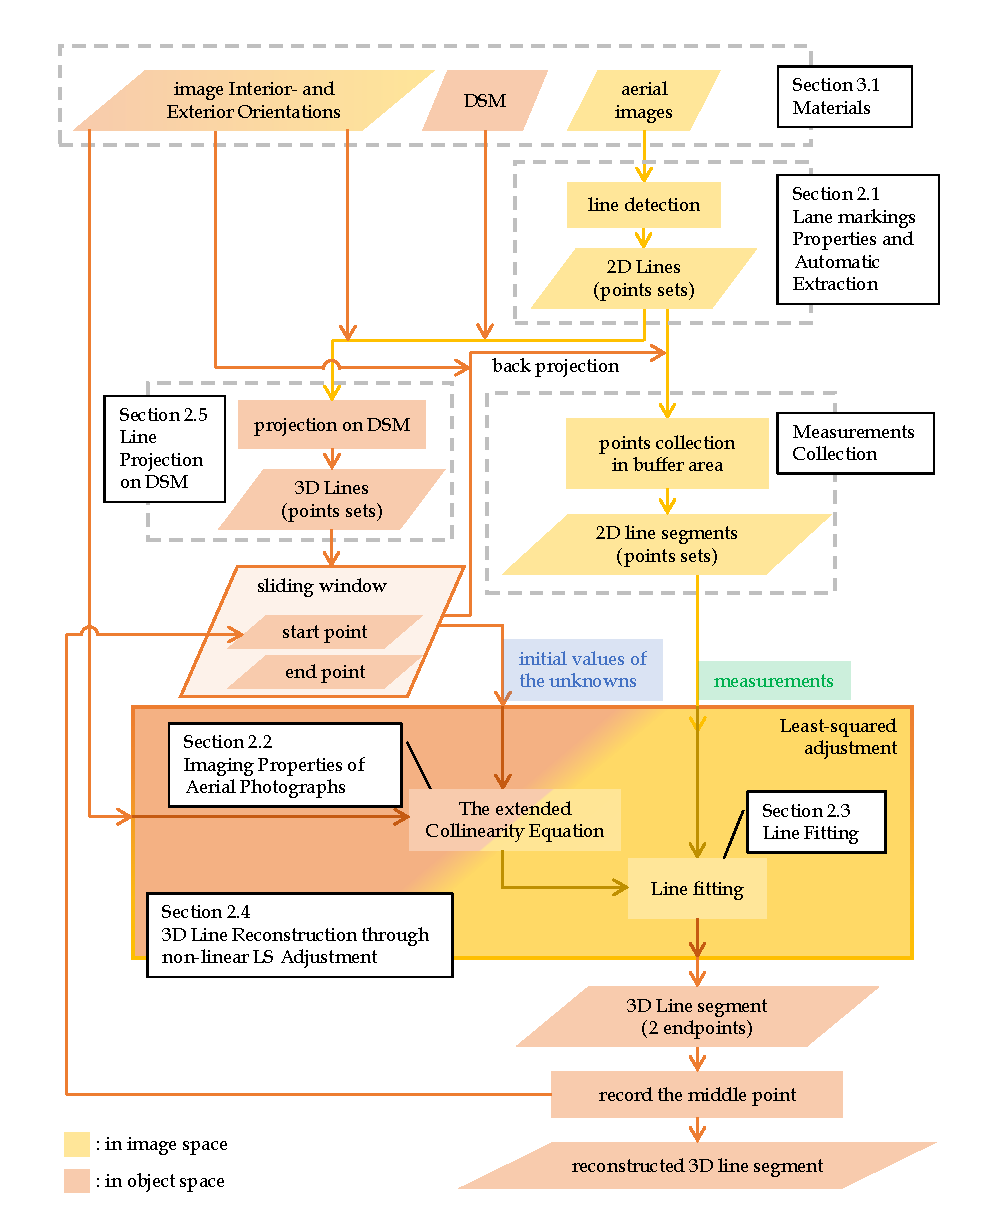
\includegraphics[width=\textwidth]{workflow.pdf}
  \caption{\small The work flow}
  \label{fig:FlowChart}
\end{figure}

\clearpage


%%%%%%%%%%%%%%%%%%%%%%%%%%%%%%%%%%%%%%%%%%%%%%%%%%%%%%%%
\section{Lane markings Properties and Automatic Extraction}
\label{sec:LineExtraction}
% Missing some small review about alternative methods?
% This chapter should be much more detailled.
The appearance of lane markings on German roads including line type, color and width is specified depending on the road type. Different line types of lane markings are shown in \cref{fig:LaneMarkingTypes} and their line widths are defined in \cref{tab:LaneMarkingWidths}. As shown in \cref{tab:DashedLaneMarkingLengths}, the dashed lane markings on motorways are of 6 meter length.
% https://de.wikipedia.org/wiki/Fahrbahnmarkierung#Eigenschaften
% Richtlinien für die Markierung von Straßen (RMS) Teil 1

Because of the appearance, the problem of lane marking detection can be treated as a line detection problem. We restrict the proposed framework to lane markings with single white lines (dashed or continuous) of 0.3 meter width. Other types like in restricted zone, double lines, parking areas, temporal yellow lines in construction sites etc, are excluded.% https://www.transchool.lee.army.mil/adso/documents/zeichen.pdf

The principle to extract line features is to firstly derive the line direction for each pixel by using partial derivatives of a Gaussian smoothing kernel. Pixels that have a local maximum in the second directional derivative perpendicular to the line direction are marked as line points. By thresholding their second directional derivative values, the accepted line points are then linked and connected.
% C. Steger: “Extracting Curvilinear Structures: A Differential Geometric Approach”. In B. Buxton, R. Cipolla, eds., “Fourth European Conference on Computer Vision”, Lecture Notes in Computer Science, Volume 1064, Springer Verlag, pp. 630-641, 1996. 
% C. Steger: “Extraction of Curved Lines from Images”. In “13th International Conference on Pattern Recognition”, Volume II, pp. 251-255, 1996. 
% C. Steger: “An Unbiased Detector of Curvilinear Structures”. IEEE Transactions on Pattern Analysis and Machine Intelligence, vol. 20, no. 2, pp. 113-125, 1998
The resultant connected points which compose a line are of sub-pixel precision. \cref{fig:LineExtraction} shows the extracted lines on the masked original image.
% http://www.mvtec.com/doc/halcon/11/en/lines_gauss.html

\begin{figure}
\centering
\subfloat[\small Continuous line]{\fbox{
\includegraphics[width=0.3\textwidth, trim={0 150 0 150},clip=true]{Laengsmarkierung_durchgehend.pdf}}}
\quad
\subfloat[\small Dashed line]{\fbox{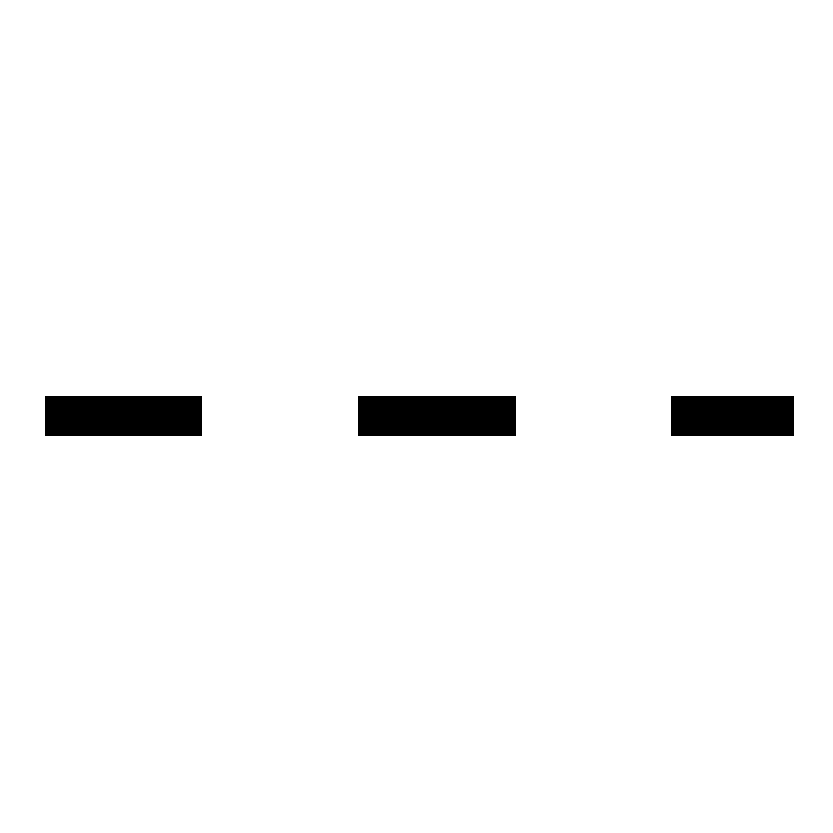
\includegraphics[width=0.3\textwidth, trim={0 150 0 150},clip=true]{Laengsmarkierung_unterbrochen.pdf}}}
\newline
\subfloat[\small Continuous and dashed double lines]{\fbox{
\includegraphics[width=0.3\textwidth, trim={0 150 0 150},clip=true]{Laengsmarkierung_unterbrochen_durchgehend.pdf}}}
\quad
\subfloat[\small Continuous double lines]{\fbox{
\includegraphics[width=0.3\textwidth, trim={0 150 0 150},clip=true]{Laengsmarkierung_durchgehend_doppelt.pdf}}}
\quad
\subfloat[\small Dashed double lines]{\fbox{
\includegraphics[width=0.3\textwidth, trim={0 150 0 150},clip=true]{Laengsmarkierung_unterbrochen_doppelt.pdf}}}
\caption{\small Line types of lane markings [source RMS Teil 1]}
% https://de.wikipedia.org/wiki/Fahrbahnmarkierung
% Richtlinien für die Markierung von Straßen (RMS) Teil 1
\label{fig:LaneMarkingTypes}
\end{figure}
\setlength{\floatsep}{16pt plus 1.0pt minus 2.0pt}
\begin{table}
    \centering
    \begin{tabular}{l|cc}
    \toprule
           & motorways\footnote{and corresponding roads in the sense of the VwV-StVO to § 42 to mark 330 (motorway) II}  & other roads\\
    \midrule
    narrow lines & $0.15$ [m] & $0.12$ [m] \\
    wide lines   & $0.30$ [m] & $0.25$ [m] \\
    \bottomrule
    \end{tabular}
    \caption{\small Widths of lane markings [source RMS Teil 1]}
    \label{tab:LaneMarkingWidths}
% Der Deutsche Verkehrssicherheitsrat
% https://www.dvr.de/download/publikationen-schriftenreihe-17.pdf
% Richtlinien für die Markierung von Straßen (RMS) Teil 1
\end{table}
\setlength{\floatsep}{16pt plus 1.0pt minus 2.0pt}
\begin{table}
    \centering
    \begin{tabular}{l|ccc}
    \toprule
          & motorways & \multicolumn{2}{c}{other roads}\\
          &           & in town & out of town\\
    \midrule
    line / gap  & $6$ [m] / $12$ [m] & $3$ [m] / $6$ [m] & $4$ [m] / $8$ [m]\\
    \bottomrule
    \end{tabular}
    \caption{\small Lengths of dashed lane markings with ratio 1:2 [source RMS Teil 1]}
    \label{tab:DashedLaneMarkingLengths}
% Der Deutsche Verkehrssicherheitsrat
% https://www.dvr.de/download/publikationen-schriftenreihe-17.pdf
% Richtlinien für die Markierung von Straßen (RMS) Teil 1
\end{table}

\begin{figure}
  \centering
  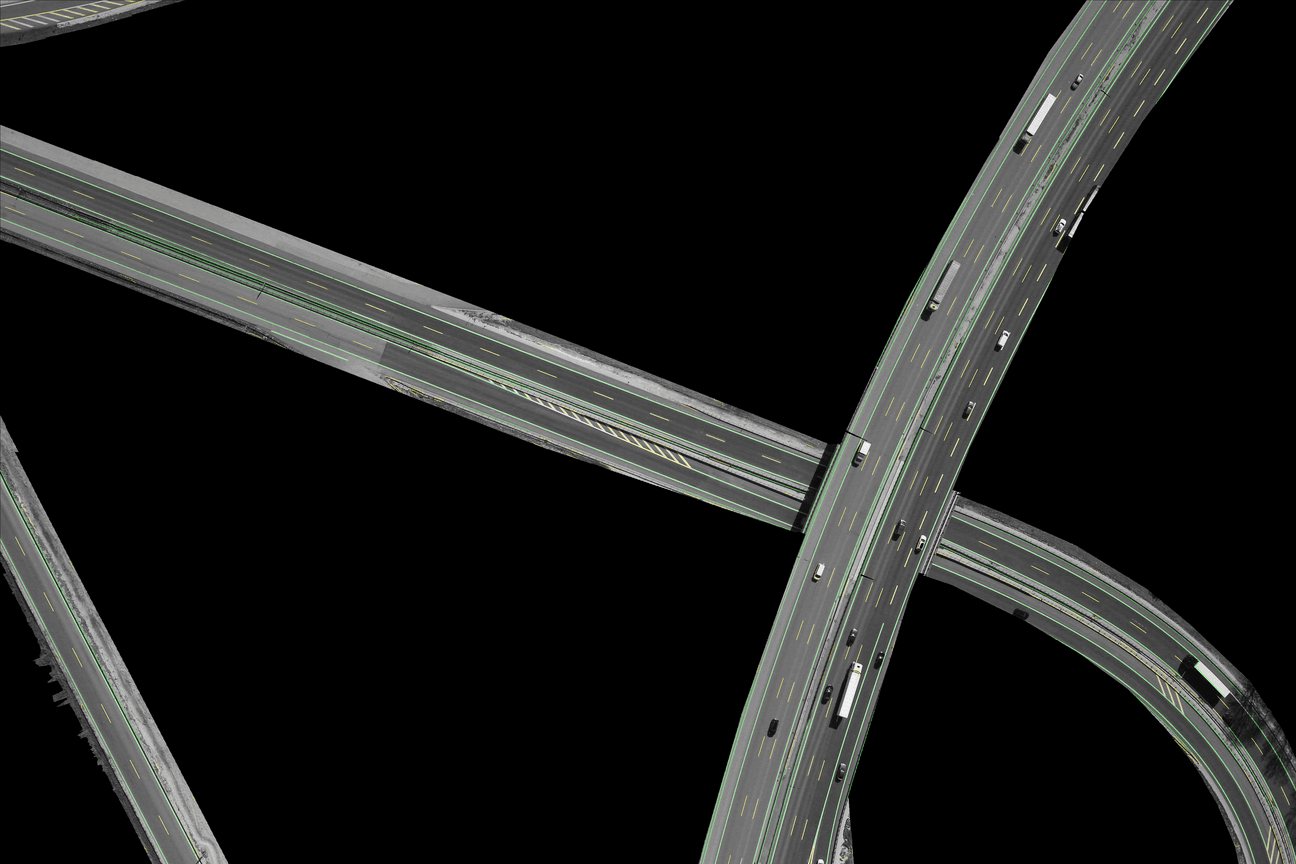
\includegraphics[width=0.7\textwidth, trim=750 250 200 320,clip]{ML1234_extlines_rsz.png}
  \caption{\small Lane markings Extraction. The extracted long lane-lines are marked in green and the dashed ones are in yellow.  Note that both cases are reconstructed into 3D with the same framework; different colors here are only for illustration.}
  \label{fig:LineExtraction}
\end{figure}



%%%%%%%%%%%%%%%%%%%%%%%%%%%%%%%%%%%%%%%%%%%%%%%%%%%%%%%%
\section{Imaging Properties of Aerial Photographs}
\label{sec:Geometry}

This section describes the geometric model of the projection of 3D points into the image generated by a real camera. We first restrict the discussion in \cref{subsec:Collinearity} to central perspective projection where the collinearity equation originate from. We then model deviations from this model, addressing real cameras with imperfect lenses, in \cref{subsec:LensDistortion}.

\subsection{Collinearity Equations}
\label{subsec:Collinearity}
We assume frame photography, i.e. photographs exposed on a frame chip in one instant, and assume central projection model with cameras that have a single viewpoint and a planar sensor and being straight line-preserving. Collinearity indicates the condition that the image point (on the sensor plate of the camera), the observed point (in object space) and the projection center of the camera were aligned at the moment the picture was taken. Every measured point leads to two collinearity equations, describing transformations from object space to image coordinates:
\begin{equation} \label{eq:collinearity}
\begin{split}
x = x_0 -c \dfrac {R_{11}(X-X_0) + R_{21}(Y-Y_0) + R_{31}(Z-Z_0)} {R_{13}(X-X_0) + R_{23}(Y-Y_0) + R_{33}(Z-Z_0)} \\
y = y_0 -c \dfrac {R_{12}(X-X_0) + R_{22}(Y-Y_0) + R_{32}(Z-Z_0)} {R_{13}(X-X_0) + R_{23}(Y-Y_0) + R_{33}(Z-Z_0)}
\end{split}
\end{equation}
where\newline
$(x, y)$: image coordinates of the point \newline
$(x_0, y_0)$: image coordinates of principal point \newline
$c$: principal distance; focal length \newline
$(X, Y, Z)$: object coordinates of the point \newline
$(X_0, Y_0, Z_0)$: object coordinates of projection center \newline
$R_{11},...,R_{33}$: elements of the rotation matrix R (orthogonal 3$\times$3-matrix from object space to image space, with 3 independent angles $\omega$, $\phi$ and $\kappa$)

\subsection{Lens Distortion Correction}
\label{subsec:LensDistortion}

An original image appears to have some degree of deviations from perspective mapping due to lens distortion, lens refraction or non-planarity of the sensor surface. There are several models to describe these perturbing effects and can be used to undistort the images, resulting in rectified images which are now straight line-preserving.
 
A subset of physical distortion model [Fraser 1997] is chosen, with two radial symmetric distortion parameters $A_1$ and $A_2$, two asymmetric parameters $B_1$ and $B_2$, and a scaling $C1$ and an affine shearing parameter $C_2$. Assuming $x$ and $y$ to be the distorted image coordinates, the corrections $\Delta x$ and $\Delta y$ are then calculated by the following equations:
\begin{equation} \label{eq:LensDistortion}
\begin{split}
\Delta x &= x_p + A_1x_*(r^2-R_0^2) + A_2x_*(r^4-R_0^4) + B_1(r^2+2x_*^2) + B_22x_*y+C_2y \\
\Delta y &= y_p + A_1y  (r^2-R_0^2) + A_2y  (r^4-R_0^4) + B_1(r^2+2y^2)   + B_22x_*y
\end{split}
\end{equation}
with $r=\sqrt{x_*^2+y^2}$, $x_*=\dfrac{x}{C_1}$ and radius\footnote{At the radius $R_0$ the radial symmetric distortion is zero by definition, which avoids too high distortion values at the edges and reduces the correlation with the focal length.} $R_0$ being set %to 0.014m which corresponds 
to a third of the sensor diagonal.

The undistorted image coordinates $x\prime$ and $y\prime$ are then calculated by
\begin{equation} \label{eq:undistortedimgcoord}
\begin{split}
x\prime=x+\Delta x \\
y\prime=y+\Delta y
\end{split}
\end{equation}

\subsection{Extended Collinearity Equation}
\label{subsec:ExtendedCollinearity}
As real cameras generally only approximate the perspective camera model, lens distortion correction can be additionally included in the collinearity model, attempting to correct the pixel position so that they obey the perspective model with sufficient accuracy.[W. Förstner et al. 2016]% The reference is not the original one

By inserting \eqref{eq:collinearity} and \eqref{eq:LensDistortion} into \eqref{eq:undistortedimgcoord} , the relationship between a 3D point $\mathbf{P}(X, Y, Z)$ and its corresponding distorted image coordinates $\mathbf{p}(x,y)$ can be described as
\begin{equation} \label{eq:expandedcollinearity}
\begin{split}
x =& x_0-c\dfrac{R_{11}(X-X_0)+R_{21}(Y-Y_0)+R_{31}(Z-Z_0)}{R_{13}(X-X_0)+R_{23}(Y-Y_0)+R_{33}(Z-Z_0)} \\
&-(x_p + A_1x_*(r^2-R_0^2) + A_2x_*(r^4-R_0^4) + B_1(r^2+2x_*^2) + B_22x_*y+C_2y)\\
y =& y_0-c\dfrac{R_{12}(X-X_0)+R_{22}(Y-Y_0)+R_{32}(Z-Z_0)}{R_{13}(X-X_0)+R_{23}(Y-Y_0)+R_{33}(Z-Z_0)} \\
&-(y_p + A_1y  (r^2-R_0^2) + A_2y  (r^4-R_0^4) + B_1(r^2+2y^2)   + B_22x_*y)
\end{split}
\end{equation}

To express \eqref{eq:expandedcollinearity} shortly, a function $\mathcal{G}$ is defined as
\begin{equation} \label{eq:Gfunction}
\mathbf{p} = \mathcal{G}(\mathbf{q},\mathbf{P}) 
\end{equation}

which takes the interior and exterior orientations as well as the lens distortion parameters of a camera $\mathbf{q}(x_0,y_0,c,X_0,Y_0,Z_0,R_{11},...,R_{33},A_1,A_2,B_1,B_2,C_1,C_2)$ and the position of a 3D point $\mathbf{P}(X, Y, Z)$, and returns the corresponding distorted image coordinates $\mathbf{p}(x,y)$.


%%%%%%%%%%%%%%%%%%%%%%%%%%%%%%%%%%%%%%%%%%%%%%%%%%%%%%%%
\section{Line Fitting}
\label{sec:LineFitting}

Line fitting is the process of constructing a infinite straight line that has a best fit to a 2D dataset. One of the approaches is linear regression which attempts to find the linear function that "best" predicts the dependent variable values as a function of the independent variable. In this work, "best" predict will be understood as in the \gls{ls} approach: minimization of the sum of squared residuals (differences between the measured and the estimated values of the dependent variable).

In the case of standard linear regression, the regressor $y$ is assumed error free, inconsistencies\footnote{The word "inconsistencies" indicates the unobserved random errors, also called as measurement errors.} are only for the dependent variable $x$. Geometrically it means that the horizontal distances from observed data to the fitted line is minimized. To minimize the perpendicular distances from the data points to the regression line, a orthogonal regression model is derived in \cref{subsec:OrthogonalRegression}.

For a later combination with point-wise extended collinearity equation \eqref{eq:Gfunction} in next section, we aim to fit the line equation in two-point form to the observed dataset. 
% extracted lines produced in \cref{sec:LineExtraction} (in forms of sets of points in image coordinates). 
For such non-linear least squares fitting purpose, a non-linear mixed model is derived in \cref{subsec:NonLinear}. % !!!!!!!!!!!!!!!!!

A functional model is unsolvable when the assumed "dependent" variable is indeed not a function of the independent variables, i.e. the assumed functional relationship does not really exist. Take an observed set of 2D points with their Cartesian coordinates $\{x_i,y_i\}^n_{i=1}$ on a vertical line $x=constant$ for example. Their $y$ values have no dependency on their $x$ values, i.e. knowledge of $x$ tells nothing about $y$. Therefore, for this dataset, the functional model $y=f(x)$ is barely solvable. In such cases, however, $x$ is a function of $y$ (which is actually a constant function) and the equation system which models the dependent variable $x$ being a function of the independent variable $y$ becomes solvable. Regarding the dataset used in this work (which will be described with more details in \cref{sec:Materials}) where the observed 2D points scatter mainly in column direction in image space, the linear relationship between $x$ and $y$ values will be setup as $x=f(y)$ to avoid weakly solvable equations system.


%\subsection{Simple Linear Regression}
%\label{subsec:LinearRegression}

%A simple linear regression model describes the linear relationship between a dependent variable and a regressors (an independent variable). By assuming the regressor $y$ being exactly measured without errors, it accounts only for errors $e_x$ in the dependent variable $x$.

%Given a dataset $\{x_i,y_i\}^n_{i=1}$ of $n$ points on a 2D plane, the model takes the form:
%\begin{equation} \label{eq:SimpleLinearRegression}
%x_i - e_{x_i} = a_0 + a_1y_i
%\end{equation}
%where the regression coefficients $a_0$ and $a_1$ are the unknown parameters to be estimated; the error variable $e_x$ is an unobserved random variable that adds noise to the linear relationship between the dependent variable $x$ and regressor $y$.
%https://en.wikipedia.org/wiki/Linear_regression#Assumptions


\subsection{Orthogonal Regression}
\label{subsec:OrthogonalRegression}
A linear regression model describes a dependent variable as a linear function of the regressor (an independent variable). Given a dataset $\{x_i,y_i\}^n_{i=1}$ of $n$ points on a 2D plane, in the case when both dependent variable $x_i$ and regressor $y_i$ are measured with errors %$e_x$ and $e_y$
, a linear regression model takes the form:
\begin{equation} \label{eq:MixModel1-1}
x_i - e_{x_i} = %a_0 + a_1(y_i-e_{y_i}) = 
a_0 + a_1\bar{y_i}
\end{equation}
where the regression coefficients $a_0$ and $a_1$ are the unknown parameters to be estimated, $\bar{y_i}$ denotes the true but unobserved regressor, and the error variable $e_{x_i}$ is an unobserved random variable that adds noise to the linear relationship between the dependent variable $x$ and true regressor $\bar{y_i}$. The true regressor $\bar{y_i}$ is observed with an error $e_{y_i}$ in the pseudo observation equation:
\begin{equation} \label{eq:MixModel1-2}
y_i-e_{y_i} = \bar{y_i}
\end{equation}
Such models, as the combination of \eqref{eq:MixModel1-1} and \eqref{eq:MixModel1-2}, that account the measurement errors in both dependent variable and regressor, are errors-in-variables models. Further more, for the case of equal error variances, i.e. when $\delta=\dfrac{\sigma_{e_x}}{\sigma_{e_y}}=1$, it is a orthogonal regression model which minimizes the %sum of squared 
perpendicular distances from the data points to the regression line.

% !!!
%As \eqref{eq:MixModel1-1} describes the relationship between observations and unknowns and \eqref{eq:MixModel1-2} describes the relationship between observations, this model is known as the mixed model or Gauss-Helmert model.
% It will be helpful to write the basic equations of the model.

\subsection{Orthogonal Regression in Two-point Form}
\label{subsec:NonLinear}

The two-point form of a infinite line in the Cartesian plane passing through the points $(x_1,y_1)$ and $(x_2,y_2)$ is given by:
\begin{equation} \label{eq:LineInTwoPointForm}
(x-x_1) = \dfrac{(x_2-x_1)}{(y_2-y_1)}\times y-y_1
\end{equation}
with $y_2\neq y_1$, where $(x,y)$ is any point on the line.

Let the unknown coordinates of two different points on a line in 2D space be $(x_1,y_1)$ and $(x_2,y_2)$ and the observed 2D points be $\{x_i,y_i\}^n_{i=1}$ with measurement errors $e_{x_i}$ and $e_{y_i}$ in both variables. The orthogonal regression model in two-point form: 
\begin{equation} \label{eq:MixModel2-1}
x_i - e_{x_i}= (x_1-\dfrac{(x_2-x_1)}{(y_2-y_1)}\times y_1) + \dfrac{(x_2-x_1)}{(y_2-y_1)}\times \bar{y_i}
\end{equation}
\begin{equation} \tag{\ref{eq:MixModel1-2} revisited}
y_i-e_{y_i} = \bar{y_i}
\end{equation}

To express \eqref{eq:MixModel2-1} and \eqref{eq:MixModel1-2} shortly, a function $\mathcal{F}$ is defined as

\begin{equation} \label{eq:Ffunction}
\hat{\mathbf{p}} = \mathcal{F}(\mathbf{p}_s,\mathbf{p}_e,y)
\end{equation}

which takes 2D coordinates of a start-point $\mathbf{p_s}(x_s,y_s)$ and an end-point $\mathbf{p_e}(x_e,y_e)$ that define an infinite line, and takes the measured y-coordinate $y$ of an image point $\mathbf{p}(x,y)$, and returns the estimated image coordinates $\mathbf{\hat{p}}(\hat{x},\hat{y})$ which lies on the infinite line $\overline{\mathbf{p_s}\mathbf{p_s}}$.

Note that as a combination of \eqref{eq:MixModel2-1} and \eqref{eq:MixModel1-2}, function $\mathcal{F}$ is actually composed of
\begin{equation} \label{eq:Ffunction_xy}
\begin{split}
\hat{x} = \mathcal{F}^x(\mathbf{p}_s,\mathbf{p}_e,y)\\
\hat{y} = \mathcal{F}^y(\mathbf{p}_s,\mathbf{p}_e,y)
\end{split}
\end{equation}

%%%%%%%%%%%%%%%%%%%%%%%%%%%%%%%%%%%%%%%%%%%%%%%%%%%%%%%%
\section{3D line reconstruction through non-linear LS Adjustment}
\label{sec:LSadj}

In this section, I describe the process of refining the position of a 3D line segment in the object space so that its back-projection in each image has a best-fit to the extracted line in the image space. To simplify the problem, a lane-marking-segment is partially reconstructed through a sliding window in the object space. Each segment is approximated by a straight line, taking into account the maximum curvature of the highway. 
The length of the sliding window depends on the expected curvature, and for motorways it was fixed to 9m …
% What about dashed lane markings in the middle? Why do you choose 9m -> compromise between robustness and minimized systematic errors.

In the sliding window, a line segment is reconstructed taking into account all the measurements (the detected lines) collected in the corresponding regions in all covering images. Only the middle point of the sliding window is then reconstructed by the least-squares estimator (see chapter xx) %!!!
and is recorded. The sliding window then moves half length forward, and the process of 3D reconstruction started again from the recorded middle point of the previous line segment. Another line segment is then reconstructed, with its middle point being recorded. These recorded middle points are in the end the nodes of the reconstructed line. The reconsideration in overlapping region makes the reconstruction more robust.
% Maybe make figure to illustrate

In \cref{subsec:ObsEqua} I firstly set up a model of observation equations. They describe the fitting of a straight line to the measurements in each covering image, where the fitting lines on different images are transformed from a single 3D straight line segment through the extended collinearity equation \eqref{eq:expandedcollinearity}.

Regarding the fact that the collinearity is a point-wise condition, a line segment is represented by its two endpoints whose object coordinates are the six unknown parameters % First mentioned here, what are the six unknowns?
in the LS model. % Which one? 
Correspondingly, the observation equations are line equations in two-point form. A line equation has however a mathematical meaning of infinite length. Therefore, some constraints on unknowns are necessary to avoid arbitrary locations of the two points on the infinite reconstructed 3D line. The constraint equations are modeled in \cref{subsec:ConEqua}.


% the measurements are collected accordingly.

\subsection{The Gauss-Markov Model with Constraints}
\label{GaussMarkovModelwithConstraints}

\paragraph{The Functional Model}
The Gauss-Markov model with constraints starts from $N$ observations $l_n$ for $U$ unknown parameters $x_u$ with $H$ constraints $h_h$ between the unknowns:
\begin{equation} \label{eq:GM-ObsEq}
\boldsymbol l+\widehat{\boldsymbol v}=\boldsymbol f(\widehat{\boldsymbol x})\quad \textnormal{or}\quad \widehat{\boldsymbol l}=\boldsymbol f(\widehat{\boldsymbol x})
\end{equation}
\begin{equation} \label{eq:GM-ConEq}
\boldsymbol h(\widehat{\boldsymbol x})=\mathbf{0}
\end{equation}

The linearized Gauss-Markov model with constraints between the unknowns is:
\begin{equation} \label{eq:GM-ObsEq-linear}
\widehat{\Delta\boldsymbol l}=\Delta\boldsymbol l+\widehat{\boldsymbol v}=\mathsf{A}\,\widehat{\Delta\boldsymbol x}
\end{equation}
\begin{equation} \label{eq:GM-ConEq-linear}
-\boldsymbol h(\widehat{\boldsymbol x}^a)=\mathsf{H^T}\widehat{\Delta\boldsymbol x}
\end{equation}
with
\begin{equation} \label{eq:GM-ObsEq-linear-l}
\Delta\boldsymbol l=\boldsymbol l-\boldsymbol f(\widehat{\boldsymbol x}^a)
\end{equation}
\begin{equation} \label{eq:GM-ObsEq-linear-x}
\widehat{\Delta\boldsymbol x}=\widehat{\boldsymbol x}-\widehat{\boldsymbol x}^a
\end{equation}

\paragraph{The Stochastic Model}




\subsection{Model of Observation Equations}
\label{subsec:ObsEqua}
% % %
% which can be further rewritten:
%Taylor expansion...(local linear approximation)
%the linear equation can also be expanded

Given a start-point $\mathbf{P}_s(X_s,Y_s,Z_s)$ and an end-point $\mathbf{P}_e(X_e,Y_e,Z_e)$ of a line segment $L$ in the object space and the camera parameters $\mathbf{q}^j$ of camera $j$. Consider the case where there are $J$ images covering this line segment. With the expanded collinearity model \eqref{eq:expandedcollinearity}, the start- and end-points of this line segment's back-projection in image $j$ have the image coordinates $\mathbf{p}^j_s(x^j_s,y^j_s)$ and $\mathbf{p}^j_e(x^j_e,y^j_e)$:
\begin{equation} \label{eq:obsmodel-collinearity}
\begin{split}
\mathbf{p}^j_s = \mathcal{G}(\mathbf{q}^j,\mathbf{P}_s)\\
\mathbf{p}^j_e = \mathcal{G}(\mathbf{q}^j,\mathbf{P}_e)
\end{split}
\qquad
\begin{split}
\forall j=1,2,...J
\end{split}
\end{equation}

%%%%%%%%%%%%%%% !!!!!!!!!!!!!!!!!! %%%%%%%%%%%%%%%%
%Let $l^j$ be the corresponding line segment of $L$ being extracted (observed) on image $j$. Given a dataset $\{x^j_{l,i},y^j_{l,i}\}^{N^j_l}_{i=1}$ of $N^j_l$ points on line segment $l^j$. Rewriting the orthogonal regression model \cref{eq:MixModel2-1} and \cref{eq:MixModel1-2} in the structure of the Gauss-Markov model gives the observation equations in vector form:

%\begin{equation} \label{eq:Ffunction}
%\mathbf{l}+\hat{\mathbf{v}}=\mathbf{f}(\hat{\mathbf{x}}):\quad
%\begin{bmatrix}
% x^j_{l,i} + \hat{e}_{x^j_{l,i}}\\[0.3em]
% y^j_{l,i} + \hat{e}_{y^j_{l,i}}\\[0.3em]
%\end{bmatrix}
%=
%\begin{bmatrix}
%(\hat{x}^j_s-\dfrac{(\hat{x}^j_e-\hat{x}^j_s)}{(\hat{y}^j_e-\hat{y}^j_s)}\times \hat{y}^j_s) + \dfrac{(\hat{x}^j_e-\hat{x}^j_s)}{(\hat{y}^j_e-\hat{y}^j_s)}\times \hat{\bar{y}}_{l,i}\\
%\hat{\bar{y}}_{l,i}
%\end{bmatrix}
%\end{equation}
%which estimates a start-point $\mathbf{p_s}(x_s,y_s)$ and an end-point $\mathbf{p_e}(x_e,y_e)$ that define a infinite line in image space so that the observed image coordinates $\hat{\mathbf{p}}^j_{l,i}(\hat{x}^j_{l,i},\hat{y}^j_{l,i})$ on defined by . % !!!!!!!!!!!!!!!!!


%%%%%%%%%%%%%%% !!!!!!!!!!!!!!!!!! %%%%%%%%%%%%%%%%

Let $l^j$ be the corresponding line segment of $L$ being extracted (observed) on image $j$. Given a dataset $\{x^j_{l,i},y^j_{l,i}\}^{N^j_l}_{i=1}$ of $N^j_l$ points on line segment $l^j$, their estimated image coordinates $\hat{\mathbf{p}}^j_{l,i}(\hat{x}^j_{l,i},\hat{y}^j_{l,i})$ on the infinite line $\overline{\mathbf{p}^j_s,\mathbf{p}^j_e}$ computed from the orthogonal regression model \eqref{eq:Ffunction} are:
\begin{equation} \label{eq:obsmodel-linefitting}
\hat{\mathbf{p}}^j_{l,i} = \mathcal{F}(\mathbf{p}^j_s,\mathbf{p}^j_e,y^j_{l,i})
\qquad
\forall i=1,2,...N^j_l
\end{equation}
%%%%%%%%%%%%%%%

Combining \eqref{eq:obsmodel-collinearity} with \eqref{eq:obsmodel-linefitting} gives function $\mathcal{H}$:
\begin{equation} \label{eq:obsmodel}
\begin{split}
\hat{\mathbf{p}}^j_{l,i} &= \mathcal{F}(\mathcal{G}(\mathbf{q}^j,\mathbf{P}_s),\mathcal{G}(\mathbf{q}^j,\mathbf{P}_e),y^j_{l,i})\\
&=\mathcal{H}(\mathbf{q}^j,\mathbf{P}_s,\mathbf{P}_e,y^j_{l,i})
\qquad
\forall i=1,2,...N^j_l,\quad\forall j=1,2,...J
\end{split}
\end{equation}
which takes camera parameters $\mathbf{q}^j(x_0,y_0,c,X_0,Y_0,Z_0,R_{11},...,R_{33},A_1,A_2,B_1,B_2,C_1,C_2)$, object coordinates of $\mathbf{P}_s$ and $\mathbf{P}_e$ which define a line $\overline{\mathbf{P}_s,\mathbf{P}_e}$, and the observed y-coordinate of the point $\mathbf{p}^j_{l,i}$ in image space, and returns the estimated image coordinates $\hat{\mathbf{p}}^j_{l,i}$ on the back projected line of $\overline{\mathbf{P}_s,\mathbf{P}_e}$.
%In \cref{eq:obsmodel}, $y^j_{l,i}, i=1,2,...N^j_l$ are the measurements, $P_s$ and $P_e$ are the unknown quantities, $\mathbf{q}^j, j=1,2,...J$ includes  interior and exterior orientations as well as the lens distortion parameters of camera $j$.\newline

Corresponding to \cref{eq:Ffunction_xy}, function $\mathcal{H}$ is composed of
\begin{equation} \label{eq:obsmodel2}
\begin{split}
\hat{x}^j_{l,i} = \mathcal{H}^x(\mathbf{q}^j,\mathbf{P}_s,\mathbf{P}_e,y^j_{l,i})\\
\hat{y}^j_{l,i} = \mathcal{H}^y(\mathbf{q}^j,\mathbf{P}_s,\mathbf{P}_e,y^j_{l,i})
\end{split}
\qquad
\begin{split}
\forall i=1,2,...N^j_l,\quad\forall j=1,2,...J
\end{split}
\end{equation}

Since the adjustment will be done "segment-wise"--- for a pair of $P_s$ and $P_e$, the measurements will be collected correspondingly. % see section ???
Thus the subscription $l$ representing specific line segment will be left out in the followings.

\clearpage
Each image gives $2\times N^j$ observation equations\footnote{Dot equal indicates inconsistencies between the measured values, $x^j_i$ and $x^j_i$, and the computed values, $\mathcal{H}^x(q^j,P_s,P_e,y^j_i)$ and $\mathcal{H}^y(q^j,P_s,P_e,y^j_i)$.}. These equations are often stacked together and written in vector form as:
\begin{equation} \label{eq:Ffunction}
\begin{bmatrix}
 x^j_1\\[0.3em]
 x^j_2\\[0.3em]
 \vdots\\[0.3em]
 x^j_{N^j}\\[0.5em]
 \arrayrulecolor{lightgray} \hline
 y^j_1\\[0.3em]
 y^j_2\\[0.3em]
 \vdots\\[0.3em]
 y^j_{N^j}\\[0.5em]
\end{bmatrix}
\doteq
\begin{bmatrix}
 \mathcal{H}^x(\mathbf{q}^j,\hat{\mathbf{P}}_s,\hat{\mathbf{P}}_e,y^j_{1})\\[0.3em]
 \mathcal{H}^x(\mathbf{q}^j,\hat{\mathbf{P}}_s,\hat{\mathbf{P}}_e,y^j_{2})\\[0.3em]
 \vdots\\[0.3em]
 \mathcal{H}^x(\mathbf{q}^j,\hat{\mathbf{P}}_s,\hat{\mathbf{P}}_e,y^j_{N^j})\\[0.5em]
 \arrayrulecolor{lightgray} \hline
 \mathcal{H}^y(\mathbf{q}^j,\hat{\mathbf{P}}_s,\hat{\mathbf{P}}_e,y^j_{1})\\[0.3em]
 \mathcal{H}^y(\mathbf{q}^j,\hat{\mathbf{P}}_s,\hat{\mathbf{P}}_e,y^j_{2})\\[0.3em]
 \vdots\\[0.3em]
 \mathcal{H}^y(\mathbf{q}^j,\hat{\mathbf{P}}_s,\hat{\mathbf{P}}_e,y^j_{N^j})\\[0.5em]
\end{bmatrix}
\begin{array}{@{\kern-\nulldelimiterspace}l@{}}
 \left.\begin{array}{@{}c@{}}\\[0.3em] \\[0.3em] \\[0.3em] \\[0.5em] \end{array}\right\} N^j\\
 \left.\begin{array}{@{}c@{}}\\[0.3em] \\[0.3em] \\[0.3em] \\[0.5em] \end{array}\right\} N^j\\
\end{array}
\end{equation}

For all covering image $j=1,2,...J$, there are $2\times\displaystyle\sum_{j=1}^{J}N^j$ observation equations. Being written in the structure of the Gauss-Markov model with constraints, corresponding to \cref{eq:GM-ObsEq}, they are expressed as:
\begin{equation} \label{eq:obsvec-allcam}
\boldsymbol l+\widehat{\boldsymbol v}=\boldsymbol f(\widehat{\boldsymbol x}):\quad
\begin{bmatrix}
 x^1_1\\[0.3em]
 \vdots\\
 x^1_{N^1}\\[0.3em]
 \arrayrulecolor{lightgray} \hline
 y^1_1\\[0.3em]
 \vdots\\
 y^1_{N^1}\\[0.3em]
 \arrayrulecolor{lightgray} \hline
 \vdots\\
 \arrayrulecolor{lightgray} \hline
 x^J_1\\[0.3em]
 \vdots\\
 x^J_{N^J}\\[0.3em]
 \arrayrulecolor{lightgray} \hline
 y^J_1\\[0.3em]
 \vdots\\
 y^J_{N^J}\\[0.3em]
\end{bmatrix}
+
\begin{bmatrix}
 \hat{e}_{x^1_1}\\[0.3em]
 \vdots\\
 \hat{e}_{x^1_{N^1}}\\[0.3em]
 \arrayrulecolor{lightgray} \hline
 \hat{e}_{y^1_1}\\[0.3em]
 \vdots\\
 \hat{e}_{y^1_{N^1}}\\[0.3em]
 \arrayrulecolor{lightgray} \hline
 \vdots\\
 \arrayrulecolor{lightgray} \hline
 \hat{e}_{x^J_1}\\[0.3em]
 \vdots\\
 \hat{e}_{x^J_{N^J}}\\[0.3em]
 \arrayrulecolor{lightgray} \hline
 \hat{e}_{y^J_1}\\[0.3em]
 \vdots\\
 \hat{e}_{y^J_{N^J}}\\[0.3em]
\end{bmatrix}
=
\begin{bmatrix}
 \mathcal{H}^x(\mathbf{q}^1,\hat{\mathbf{P}}_s,\hat{\mathbf{P}}_e,y^1_1)\\[0.3em]
 \vdots\\
 \mathcal{H}^x(\mathbf{q}^1,\hat{\mathbf{P}}_s,\hat{\mathbf{P}}_e,y^1_{N^1})\\[0.3em]
 \arrayrulecolor{lightgray} \hline
 \mathcal{H}^y(\mathbf{q}^1,\hat{\mathbf{P}}_s,\hat{\mathbf{P}}_e,y^1_1)\\[0.3em]
 \vdots\\
 \mathcal{H}^y(\mathbf{q}^1,\hat{\mathbf{P}}_s,\hat{\mathbf{P}}_e,y^1_{N^1})\\[0.3em]
 \arrayrulecolor{lightgray} \hline
 \vdots\\
 \arrayrulecolor{lightgray} \hline
 \mathcal{H}^x(\mathbf{q}^J,\hat{\mathbf{P}}_s,\hat{\mathbf{P}}_e,y^J_1)\\[0.3em]
 \vdots\\
 \mathcal{H}^x(\mathbf{q}^J,\hat{\mathbf{P}}_s,\hat{\mathbf{P}}_e,y^J_{N^J})\\[0.3em]
 \arrayrulecolor{lightgray} \hline
 \mathcal{H}^y(\mathbf{q}^J,\hat{\mathbf{P}}_s,\hat{\mathbf{P}}_e,y^J_1)\\[0.3em]
 \vdots\\
 \mathcal{H}^y(\mathbf{q}^J,\hat{\mathbf{P}}_s,\hat{\mathbf{P}}_e,y^J_{N^J})\\[0.3em]
\end{bmatrix}
\begin{array}{@{\kern-\nulldelimiterspace}l@{}}
 \left.\begin{array}{@{}c@{}}\\ \\ \\ \\ \\ \\[18pt] \end{array}\right\}2\times N^1\\
 \left.\begin{array}{@{}c@{}}\\                     \end{array}\right. \vdots     \\
 \left.\begin{array}{@{}c@{}}\\ \\ \\ \\ \\ \\[18pt] \end{array}\right\}2\times N^J\\
\end{array}
\end{equation}
\clearpage



\subsection{Model of Constraint Equations}
\label{subsec:ConEqua}

% infinitely many solutions.
% At least two constraints are needed to fix rank deficiency???.
% TO BE COMPLETED !!!!!!!!!!!!!!!!!!!!!!!!!!!!!!!!!

There are three constraints on the unknown parameters used in this work:
\begin{itemize}
\item Fixing the X-, Y-coordinates of the start-point using the approximate values:
\item [] \begin{equation} \label{eq:constraint1}
\hat{X}_s-{X_s}^0=0
\end{equation}
\begin{equation} \label{eq:constraint2}
\hat{Y}_s-{Y_s}^0=0
\end{equation}
\item Fixing the length of the line segment (i.e. constraining the relative location of the end-point):
\begin{equation} \label{eq:constraint3}
\sqrt{(\hat{X}_s-\hat{X}_e)^2+(\hat{Y}_s-\hat{Y}_e)^2+(\hat{Z}_s-\hat{Z}_e)^2}-S=0
\end{equation}
\end{itemize}

Only in the first line segment reconstruction of a long lane marking, the fixed $X_s$ and $Y_s$ values are from the initial parameter estimates derived in \cref{sec:LineProjectionOnDSM}. Starting from the second line segment, the fixed values ${X_s}^0$ and ${Y_s}^0$ depend on the previously determined values.

The constraint equations \eqref{eq:constraint1}, \eqref{eq:constraint2} and \eqref{eq:constraint3} can be stacked together and written in the structure of the Gauss-Markov model with constraints, corresponding to \cref{eq:GM-ConEq}:
\begin{equation} \label{eq:convec}
\boldsymbol h(\widehat{\boldsymbol x})=\mathbf{0}:\quad
\begin{bmatrix}
 \hat{X}_s-{X_s}^0\\[0.3em]
 \hat{Y}_s-{Y_s}^0\\[0.3em]
 \sqrt{(\hat{X}_s-\hat{X}_e)^2+(\hat{Y}_s-\hat{Y}_e)^2+(\hat{Z}_s-\hat{Z}_e)^2}-S\\[0.3em]
\end{bmatrix}
=
\begin{bmatrix}
 0\\[0.3em]
 0\\[0.3em]
 0\\[0.5em]
\end{bmatrix}
\end{equation}


\subsection{The Gauss-Markov Model with Constraints}
\label{subsec:LSadj}
% Add the relevant equations
% This chapter is difficult to read, more detailed!?
%
A non-linear equation system is approximated to be locally linear with small step size of the unknown quantities. Through a linearized form of the equation system, for example Taylor's polynomial expansion, it turns to solve for the increments of unknowns instead of the unknowns themselves, where linear LS adjustment is applied iteratively until convergence is achieved. Depending on the configuration and initial parameters chosen, the nonlinear fit may have good or poor convergence properties.



% In this work, both the observation equations and constraint equations are linearized, i.e. all equations are expanded to Taylor's polynomials.



% 2.5.3 non-linear mixed model with constraints...
% 2.5.3.1 The Model and Its Linearization
% local linear
% combine the obs & con model, linearization
% 2.5.3.2 The Solution of the linearized problem

% system solvable when J>1 and well distributed, 





% % %
% derive matrices
% extended normal equation matrix N*


%%%%%%%%%%%%%%%%%%%%%%%%%%%%%%%%%%%%%%%%%%%%%%%%%%%%%%%%
\section{Line Projection on the DSM (Determination of Initial Parameter Estimates)}
\label{sec:LineProjectionOnDSM}

As the equation system in \cref{sec:LSadj} may exhibit multiple local minimum, a "correct" initial approximation of the unknowns is required for convergence to the correct solution. To provide such initial 3D line segment, the extracted line features derived in \cref{sec:LineExtraction} can be projected onto DSM based on the bundle adjusted exterior and interior orientations.

Given image coordinates $\mathbf{p}(x,y)$ of a point and (bundle-adjusted) image orientations $\mathbf{q}$, there is still one degree of freedom in extended collinearity equation \eqref{eq:Gfunction} on solving object coordinates $\mathbf{P}(X,Y,Z)$. Combined with the usage of DSM, which provides the height information $Z$ given a position $(X,Y)$, the corresponding object coordinates can be solved iteratively until the increment $\Delta Z$ small enough, i.e. convergence achieved. % Equation for dZ

Considering that the DSM is raster (discrete) whereas $X$ and $Y$ have continuous numerical values, the DSM height is bilinear interpolated during the iterative process.

%Given image coordinates of an image point and an initial Z-value $Z_{initial}$, the 
%With the following work flow:

%pseudo code:

%x,y = a set of points (detected line);		// unit: [pixel], in image coordinates
%Z_ini = 500;						// unit: [meter], in world coordinates
%while( ( Z_new – Z_ini ) < convergentthreshold )
%	(X,Y) = camera.img2geo(x,y,Z_ini);	// X,Y in world coordinates
%	Z_new = DSM.Get_height(X,Y);		// Z_new in world coordinates
%end
%return (X,Y,Z_new);

%\begin{Algorithmus} 
%\caption{Line Projection on DSM}
%\label{alg:LineProjectionOnDSM}
%\begin{algorithmic}
%\Procedure{Sample}{$a$,$v_e$}
%  \State $\mathsf{parentHandled} \gets (a = \mathsf{process}) \lor \mathsf{visited}(a'), (a',c,a) \in \mathsf{HR}$
%  \State \Comment $(a',c'a) \in \mathsf{HR}$ denotes that $a'$ is the parent of $a$
%  \If{$\mathsf{parentHandled}\,\land(\mathcal{L}_\mathit{in}(a)=\emptyset\,\lor\,\forall l \in %\mathcal{L}_\mathit{in}(a): \mathsf{visited}(l))$}
%    \State $\mathsf{visited}(a) \gets \text{true}$
%    \State $\mathsf{writes}_\circ(a,v_e) \gets
%    \begin{cases}
%      \mathsf{joinLinks}(a,v_e)                & \abs{\mathcal{L}_\mathit{in}(a)} > 0\\
%      \mathsf{writes}_\circ(p,v_e)             & \exists p: (p,c,a) \in \mathsf{HR}\\
%      (\emptyset, \emptyset, \emptyset, false) & \text{otherwise}
%    \end{cases}
%  \EndIf
%\EndProcedure
%\end{algorithmic}
%\end{Algorithmus}




% % %





%%%%%%%%%%%%%%%%%%%%%%%%%%%%%%%%%%%%%%%%%%%%%%%%%%%%%%%%
%\section{Line Grouping}
%\label{sec:}





%\begin{equation}\label{eq:test}
%a = b + c.
%\end{equation}

%\begin{equation}
%a = b + c. \tag{\ref{eq:test} revisited}
%\end{equation}




\chapter{Experimental Results and Evaluations}
\label{chap:k3}

\cref{sec:Materials} provides information about input dataset and the applied preprocessing steps. 

evaluation procedure
%The distance between the LIDAR points and the generated DSM are computed and evaluated statistically
%To evaluate the influence of the over-counting correction and MGM
%cost aggregation independently, two evaluations were performed


In \cref{sec:sd}, the correctness of the derived model is firstly verified by using simulation data without adding errors in the simulated measurements yet some biases are added in the initial values of the unknowns.

Dashed lane-lines reconstruction is presented in \cref{sec:td-short}. % 5 set of dashed lane line data
% show the differences with DSM profile
In long lane-lines reconstruction cases

%%%%%%%%%%%%%%%%%%%%%%%%%%%%%%%%%%%%%%%%%%%%%%%%%%%%%%%%
\section{Materials}
\label{sec:Materials}

\paragraph{Aerial Images}
For real-time mapping applications during disasters, mass events and traffic monitoring scenarios, the German Aerospace Center (DLR) has developed a new optical sensor system-- the 4k system-- on a helicopter from DLR. The oblique aerial images used in this work are acquired from a Canon EOS 1D-X camera, one of the three non-metric cameras in the 4k system, with an oblique viewing angle $\tau$ of 15$\degree$. The image data sets used in this work were acquired in around 500m flying height $H_{flight height}$ above ground, which leads to a GSD of ~7cm. % data of acquisition, number of images, length of flight strips,…->maybe in chapter “Experiments?

An example aerial image is shown in \cref{fig:OriImg}. \cref{tab:CameraProperties} lists the properties of this camera, and \cref{tab:SensorViewingGeometry} provides the viewing geometry information.


\begin{table}%[!h]
  \centering
  \begin{tabular}{ll}
  \toprule
                                      {} & \textbf{Canon EOS 1D-X} \\
  \midrule
  Lenses                          & Zeiss Makro Planar 2/50\\
  \\[-1em]
  Sensor / Pixel size             & Full frame CMOS / 6.944 \textmu m\\
  \\[-1em]
  \multirow{2}{*}{Image size}     & 5184$\times$3456 pixel, ratio 3:2\\
                                  & (17.9 MPix)\\
  \\[-1em]
  ISO                             & 100--204800\\
  \\[-1em]
  max. frame rate / max. images   & 14 fps/ 180 images\\
  \\[-1em]
  Exposure time                   & 30 s -- 1/8000 s\\
  \\[-1em]
  Data interface                  & LAN (EDSDK software interface)\\
  \bottomrule
  \end{tabular}
  \caption{Properties of the oblique camera }
  \label{tab:CameraProperties}
%\end{table}
\vspace{1cm}
%\begin{table}%[!h]
  \centering
  \begin{tabular}{lll}
  \toprule
                         & \textbf{RGB, 50mm lens} \\
  \midrule
  Viewing directions     & $\pm$15$\degree$\\
  \\[-1em]
  \multirow{2}{*}{FOV}   & $\pm$34$\degree$ across strip,\\
                         & $\pm$13$\degree$ along strip\\
  \\[-1em]
  Coverage @500m         & 780 m $\times$ 230 m\\
  GSD      @500m         & 6.9 cm (nadir)\\

  \bottomrule
  \end{tabular}
  \caption{Viewing geometry}
  \label{tab:SensorViewingGeometry}
\end{table}

The images used in this work are acquired with a special flight configuration at both sides of the motorway which guarantees a continuous stereo view perpendicular to the lane marking direction.\footnote{The classical photogrammetric approach on flight planning is to have several straight flight lines which cover the whole motorway in a stereo view. This would be possible in this project yet would require more flight costs and would produce many more images.} This is realized by flying at the right-hand side with respect to flying direction along the motorway, with the left oblique camera looking left-down to the motorway, in both forward and backward trip. The flight configuration is shown in \cref{fig:FlightTrajectory} on the Google Earth platform.

Besides, the forward overlap is around 70\%, and all the lane markings are covered by both strips, whereas the side overlap depends on the distance of flight strips, which are a result of the pilots navigation ability and other influences, like wind. Nevertheless, the motorway in its entire width was covered by the two flight strips. Altogether, this results in approximately 8-image coverage in road areas. 

\begin{figure}%[!h]
  \centering
  \subfloat[]{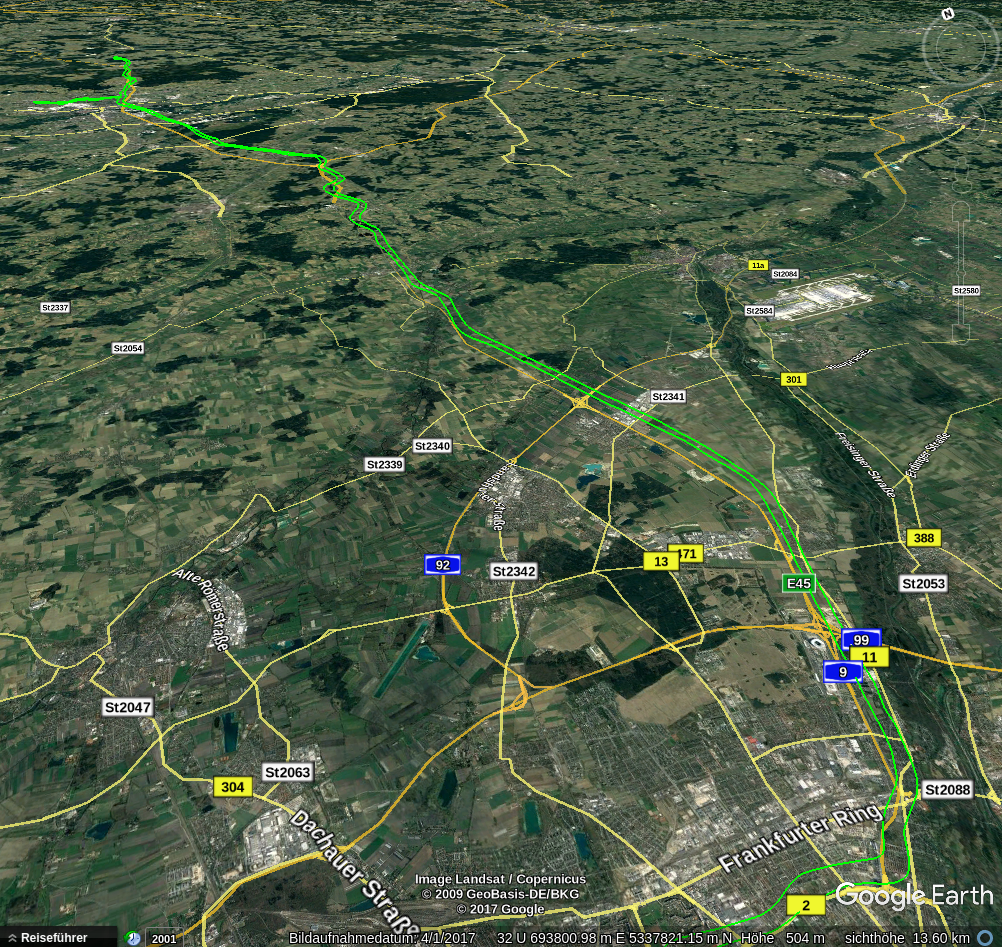
\includegraphics[height=0.45\textwidth]{FlightTrajectory5.png} \label{fig:trajectory1}}
  \subfloat[]{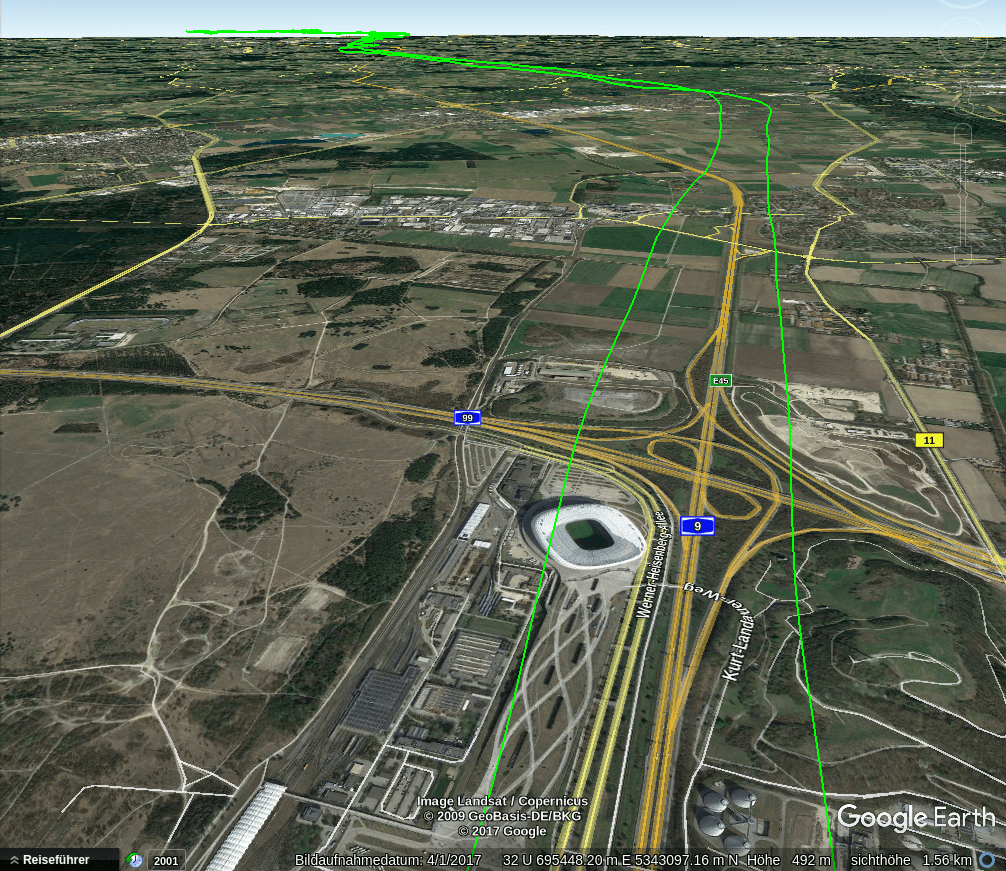
\includegraphics[height=0.45\textwidth]{FlightTrajectory3.png} \label{fig:trajectory2}}
  \caption{\small Flight trajectory of DLR helicopter visualized on the Google Earth platform. The green polyline shows the flight trajectory. \textit{Source: \textbf{Google Earth} 04/01/2017}}
  \label{fig:FlightTrajectory}
\end{figure}


\paragraph{Exterior and Interior Orientations}
The \gls{eo} of the images are directly measured by a GNSS/Inertial system IGI IId.% Missing: specification of the system, improvements by SAPOS correction,….
The EO parameters are then refined by a self-calibrating bundle adjustment. The accuracies of the exterior orientation (EO) parameters are shown in \cref{tab:EOaccuracy}. The calibrated \gls{io} parameters and their accuracies are shown in \cref{tab:IOaccuracy}. To provide an overall quality on the interior orientations: from the calibration result of interior orientations (involving lens distortion), the residuals appear non-systematic and the biggest residual $r_{max, IO}$ is around $1$ pixel.

To judge the influence of exterior and interior parameters on positioning accuracy in object space, the maximum values for each component based on the flight configuration was calculated.
The quality of interior and exterior orientation parameters set would have a maximum impact in object space for around $16.5$ [cm] in X,Y-direction:
\begin{itemize}
      \item caused by inaccurate camera position: 
      \item [] $\sqrt{\sigma_{north}^2+\sigma_{east}^2}=\sqrt{0.055^2+0.035^2}\approx0.065$ [meter]
      \item caused by inaccurate camera attitude:
      \item [] $\tan(\sqrt{\sigma_{roll}^2+\sigma_{pitch}^2})\times H_{flight height}\times\dfrac{1}{\cos^2\tau}$
      \item [] $=\tan(\sqrt{0.002^2+0.002^2})\times 500\times\dfrac{1}{\cos^215\degree}\approx0.026$ [meter]
      \item caused by inaccurate Interior Orientations:
      \item [] $r_{max, IO}\times GSD\times\dfrac{1}{\cos^2\tau}=1\times0.069\times\dfrac{1}{\cos^215\degree}\approx0.074$ [meter]
\end{itemize}
and around $9.4$ [cm] in Z-direction:
\begin{itemize}
      \item caused by inaccurate camera position:
      \item [] $\sigma_{altitude}\approx0.069$ [meter]
      \item caused by inaccurate camera attitude:
      \item [] $\tan(\sqrt{\sigma_{roll}^2+\sigma_{pitch}^2})\times H_{flight height}\times\dfrac{\sin\tau}{\cos\tau}$
      \item [] $=\tan(\sqrt{0.002^2+0.002^2})\times 500\times\dfrac{\sin15\degree}{\cos15\degree}\approx0.007$ [meter]
      \item caused by inaccurate Interior Orientations:
      \item [] $r_{max, IO}\times GSD\times\dfrac{\sin\tau}{\cos\tau}=1\times0.069\times\dfrac{\sin15\degree}{\cos15\degree}\approx0.018$ [meter]
\end{itemize}

The above information tells the positioning accuracy in object space with measurements on a single image. With corresponding measurements from multiple stereo views, which allows the intersection of multiple  rays, the positioning accuracy is expected to be improved for being overdetermined.

\begin{table}%[!h]
    \centering
    \begin{tabular}{ll|ll}
    \toprule
    position accuracies  &[meter]  & attitude accuracies & [degree]\\
    \midrule
    $\sigma_{north}$     & $0.055$ & $\sigma_{Roll}$  & $0.002$\\
    $\sigma_{east}$      & $0.035$ & $\sigma_{Pitch}$ & $0.002$\\
    $\sigma_{altitude}$  & $0.069$ & $\sigma_{Yaw}$   & $0.005$\\
    \bottomrule
    \end{tabular}
    \caption{Accuracies of Exterior Orientations}
    \label{tab:EOaccuracy}
%\end{table}
\vspace{1cm}
%\begin{table}%[!h]
    \centering
    \begin{tabular}{lr|lr|l}
    \toprule
    \multicolumn{2}{c|}{Interior Orientations}  & \multicolumn{2}{c|}{accuracies} & unit\\
    \midrule
    focal length $c$                       &   $0.051$ & $\sigma_c$      & $6.9\mathrm{e}{-7}$ & [meter]\\
    x coordinate of principal point $pp_x$ & $-42.259$ & $\sigma_{pp_x}$ & $0.167$             &[$\mu$m]\\
    x coordinate of principal point $pp_y$ & $115.384$ & $\sigma_{pp_y}$ & $0.799$             &[$\mu$m]\\
    \bottomrule
    \end{tabular}
    \caption{Interior Orientations and their accuracies}
    \label{tab:IOaccuracy}
\end{table}

\paragraph{\gls{dsm}}
For each pair of stereo images, a disparity map is generated using \gls{sgm} algorithm. With disparity's property of being inversely proportional to depth, the disparity maps can be used to derive the DSM. Since SGM is a kind of appearance-based matching, the SGM-generated DSM is noisy in lowly textured regions. 
%In most of the cases, a point in object space is covered by more than two aerial images, resulting in more than one disparity map. This leads to ambiguities on height decision during DSM generations.
%, and can be solved by simply taking the median value derived from disparity maps in odd number of disparity maps cases, and the value just lower than the median in even number cases. %This results in systematic errors of having lower height value in some parts of DSM.(The whole proof of this sentence is more complicated, I hope you will be not asked about this.)
Thus, the DSM will be used only for setting up the initial values of the work flow, and will not influence the final results of the 3D lane marking reconstruction.

The DSM has 20 cm grid spacing. \cref{fig:DSM} shows a part of the DSM. Standard deviations of the height value in this part of the DSM is shown in \cref{fig:DSMstd}. The number of stereo image pairs used for each part on the DSM is shown in \cref{fig:DSMnumber}.
% problem of higher noise at road surfaces
% Standard deviation not well visible. Maybe add number of images for this small part
\begin{figure}%[!h]
  \centering
  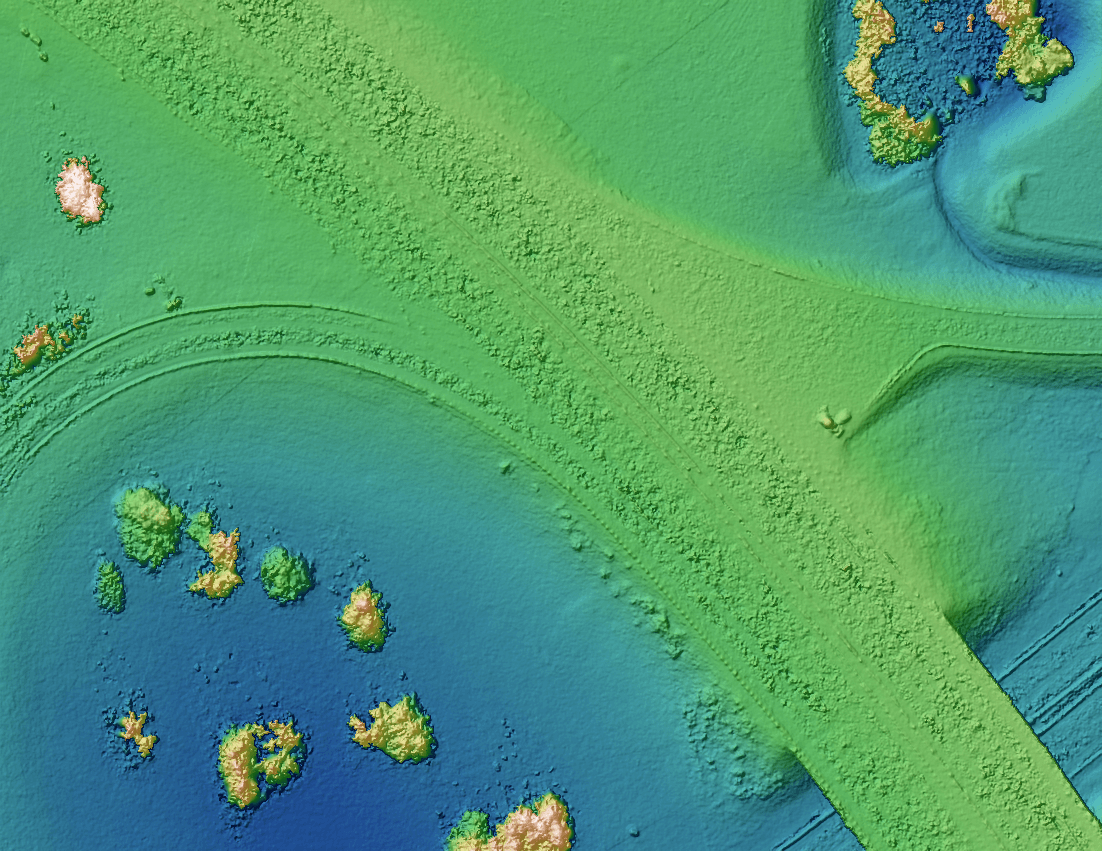
\includegraphics[width=0.8\textwidth]{DEM_A9_FINAL_PART_small_shaded.png}
  \caption{\small Part of the DSM in road area. It is noisy in the center of motorway.}
  \label{fig:DSM}
  \vspace{1cm}
  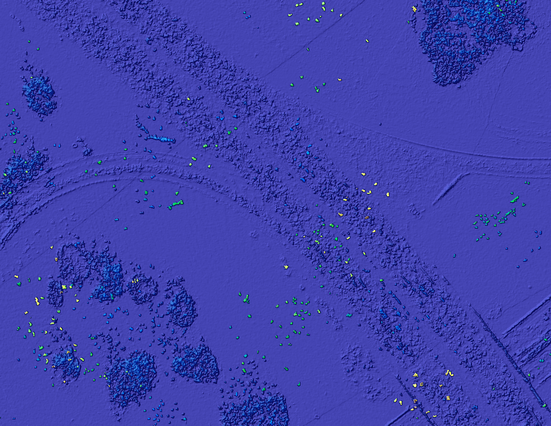
\includegraphics[width=0.8\textwidth]{DEM_A9_STD_small_terrain.png}
  \caption{\small Standard deviations of the height value of the DSM in road area. It has higher value in the center of motorway.}
  \label{fig:DSMstd}

\end{figure}

\begin{figure}%[!h]
  \centering
  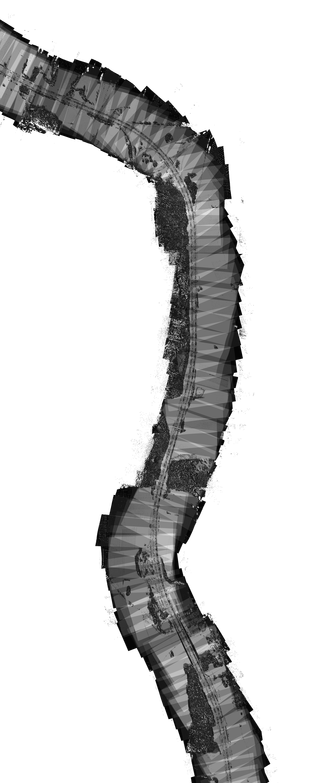
\includegraphics[width=0.5\textwidth]{DEM_A9_NUM_scaled_s.png}
  \caption{\small Distribution of stereo pairs used for DSM generation. Lighter color indicates more stereo pairs are used in that area. Maximum 27 stereo pairs are used for one pixel.}%%%%%%%%
  \label{fig:DSMnumber}
\end{figure}


\paragraph{Orthorectified Images}
The orthorectified images are processed using the DSM and the interior and exterior orientations derived from the bundle adjustment. They are georeferenced and the scale is uniform. One of the orthorectified images is shown in \cref{fig:OrthoImg}. The orthorectified images are only used for setting up initial values and used as intermediary step for processing the road masks, but do not influence the results of 3D lane marking reconstruction.
% Maybe a nice place, to visualize the DSM error on the lane marking projections…

\paragraph{Road Masks}
Road segments are masked out from original images based on \gls{osm} data: Firstly, the rasterized road segments from OSM data are written with 25 meter buffer width around road axes into orthorectified images. By back-projecting the mask from orthorectified image to original image using the 3D information from the DSM, it can then be used to mask out the road regions on the original images, as shown in \cref{fig:MaskedImg}.

\begin{figure}%[!h]
  \parbox{.475\linewidth}{
    \centering
    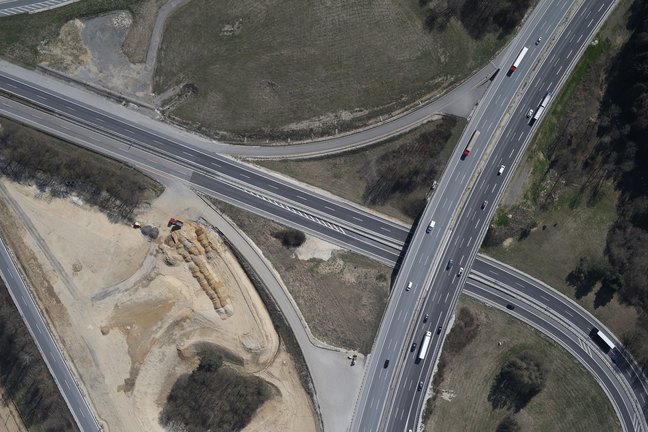
\includegraphics[width=0.45\textwidth]{L1234_rsz.png}
    \caption{\small Original Image}
    \label{fig:OriImg}
  }
  \quad
  \parbox{.475\linewidth}{
    \centering
    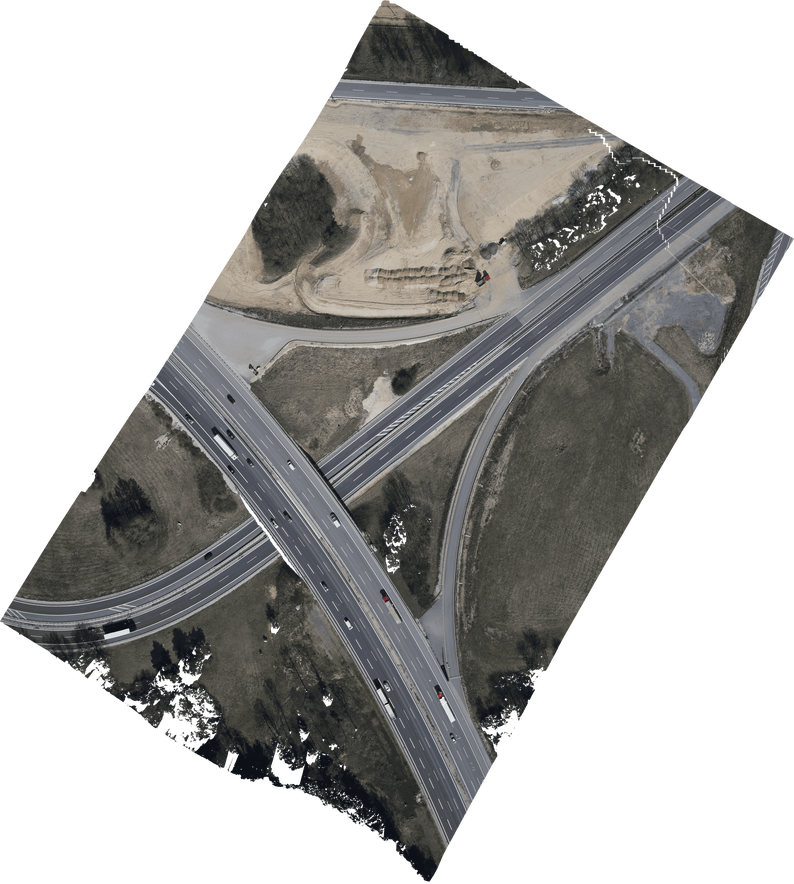
\includegraphics[width=0.45\textwidth]{OL1234_rsz.png}
    \caption{\small Orthorectified Image}
    \label{fig:OrthoImg}
  }
  \centering
  \parbox{.7\linewidth}{
    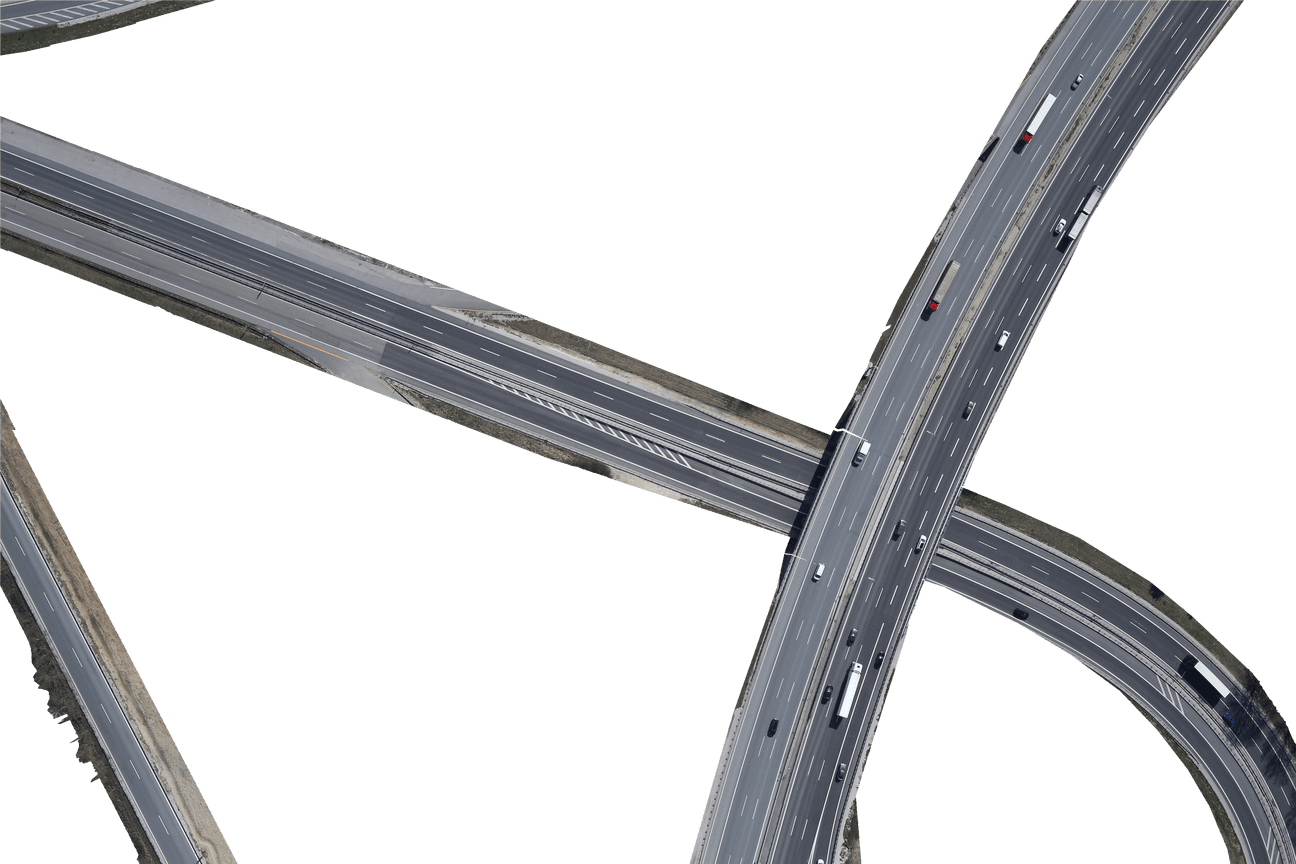
\includegraphics[width=0.7\textwidth]{ML1234_rsz.png}
    \caption{\small Masked Image}
    \label{fig:MaskedImg}
  }
\end{figure}

\clearpage
%%%%%%%%%%%%%%%%%%%%%%%%%%%%%%%%%%%%%%%%%%%%%%%%%%%%%%%%
\section{Preprocessing}
\label{sec:preprocessing}

In lane marking extraction step, the $\sigma$ value for Gaussian smoothing is set to be 1.8 % From HALCON Referenz: For the choice of the thresholds High and Low one has to keep in mind that the second directional derivative depends on the amplitude and width of the line as well as the choice of Sigma. Thus: you must set this value depending on the lane marking width?
to slightly suppress the noise in images.
The extracted lines of length less than 70 pixels are rejected % why
regarding the fact that a dashed lane-line is no longer than 6 meter which is correspondingly 87 pixels with GSD of 6.9 cm.
% http://www.mvtec.com/doc/halcon/11/en/lines_gauss.html
% https://www.dvr.de/download/publikationen-schriftenreihe-17.pdf

table:
simu.case1: noisy measurements and biased initial values of the unknowns

covering images, observations, unknowns, redundancies, 


%%%%%%%%%%%%%%%%%%%%%%%%%%%%%%%%%%%%%%%%%%%%%%%%%%%%%%%%
\section{Simulation}
\label{sec:simulation}
This section aims to verify the correctness of the derived LS model using simulation data. The used materials are as described in \cref{sec:Materials}. Only the measurements (the image coordinates of the extracted lines), the true and approximate values of the unknowns (the object coordinates of a line segment) in the non-linear LS model are simulated, as described in \cref{subsec:simudata}.

\cref{subsec:simuresult} aims to check if the iteration scheme converges to the correct solution given imperfect initial values of the unknowns. This subsection also presents the significant height differences between the approximate and the reconstructed line segments, indicating the necessity of refinement base on image triangulation.
%\cref{subsec:simuresult-2} checks, without the influences from camera parameters' quality, if the derived LS model is able to resist the simulated random errors contained in the measurements.

Note that the quality of camera parameters (EO., IO. and additional parameters) do not have influences in simulation since the simulated measurements are produced with the same set of camera parameters as the set used for 3D reconstruction.



\subsection{Simulation Data}
\label{subsec:simudata}

\paragraph{The true line segment in object space}
Firstly, the object coordinates of the endpoints of a 3D line segment are defined, with 136 meters length, locating on the road surface in the test area (German highway A9) with 3 to 7 aerial images coverage. By linear interpolating several points with 0.2 meter spaces (considering DSM grid of 0.2 meter) between the two endpoints, a 3D line segment in the form of a set of 3D points is generated. This 3D line segment serves as the ground truth in the experiments in \cref{sec:simulation}. 

\paragraph{The observed line segments in image spaces}
The observations in the LS model are simulated by back-projecting the true line segment into the covering images. Gaussian random noise $e\sim\mathcal{N}(0,0.5^2)$ is added in the observations for each LS adjustment, as line extraction process is of sub-pixel accuracy. The added noise is plotted in \cref{fig:noise}

\begin{figure}
  \centering
  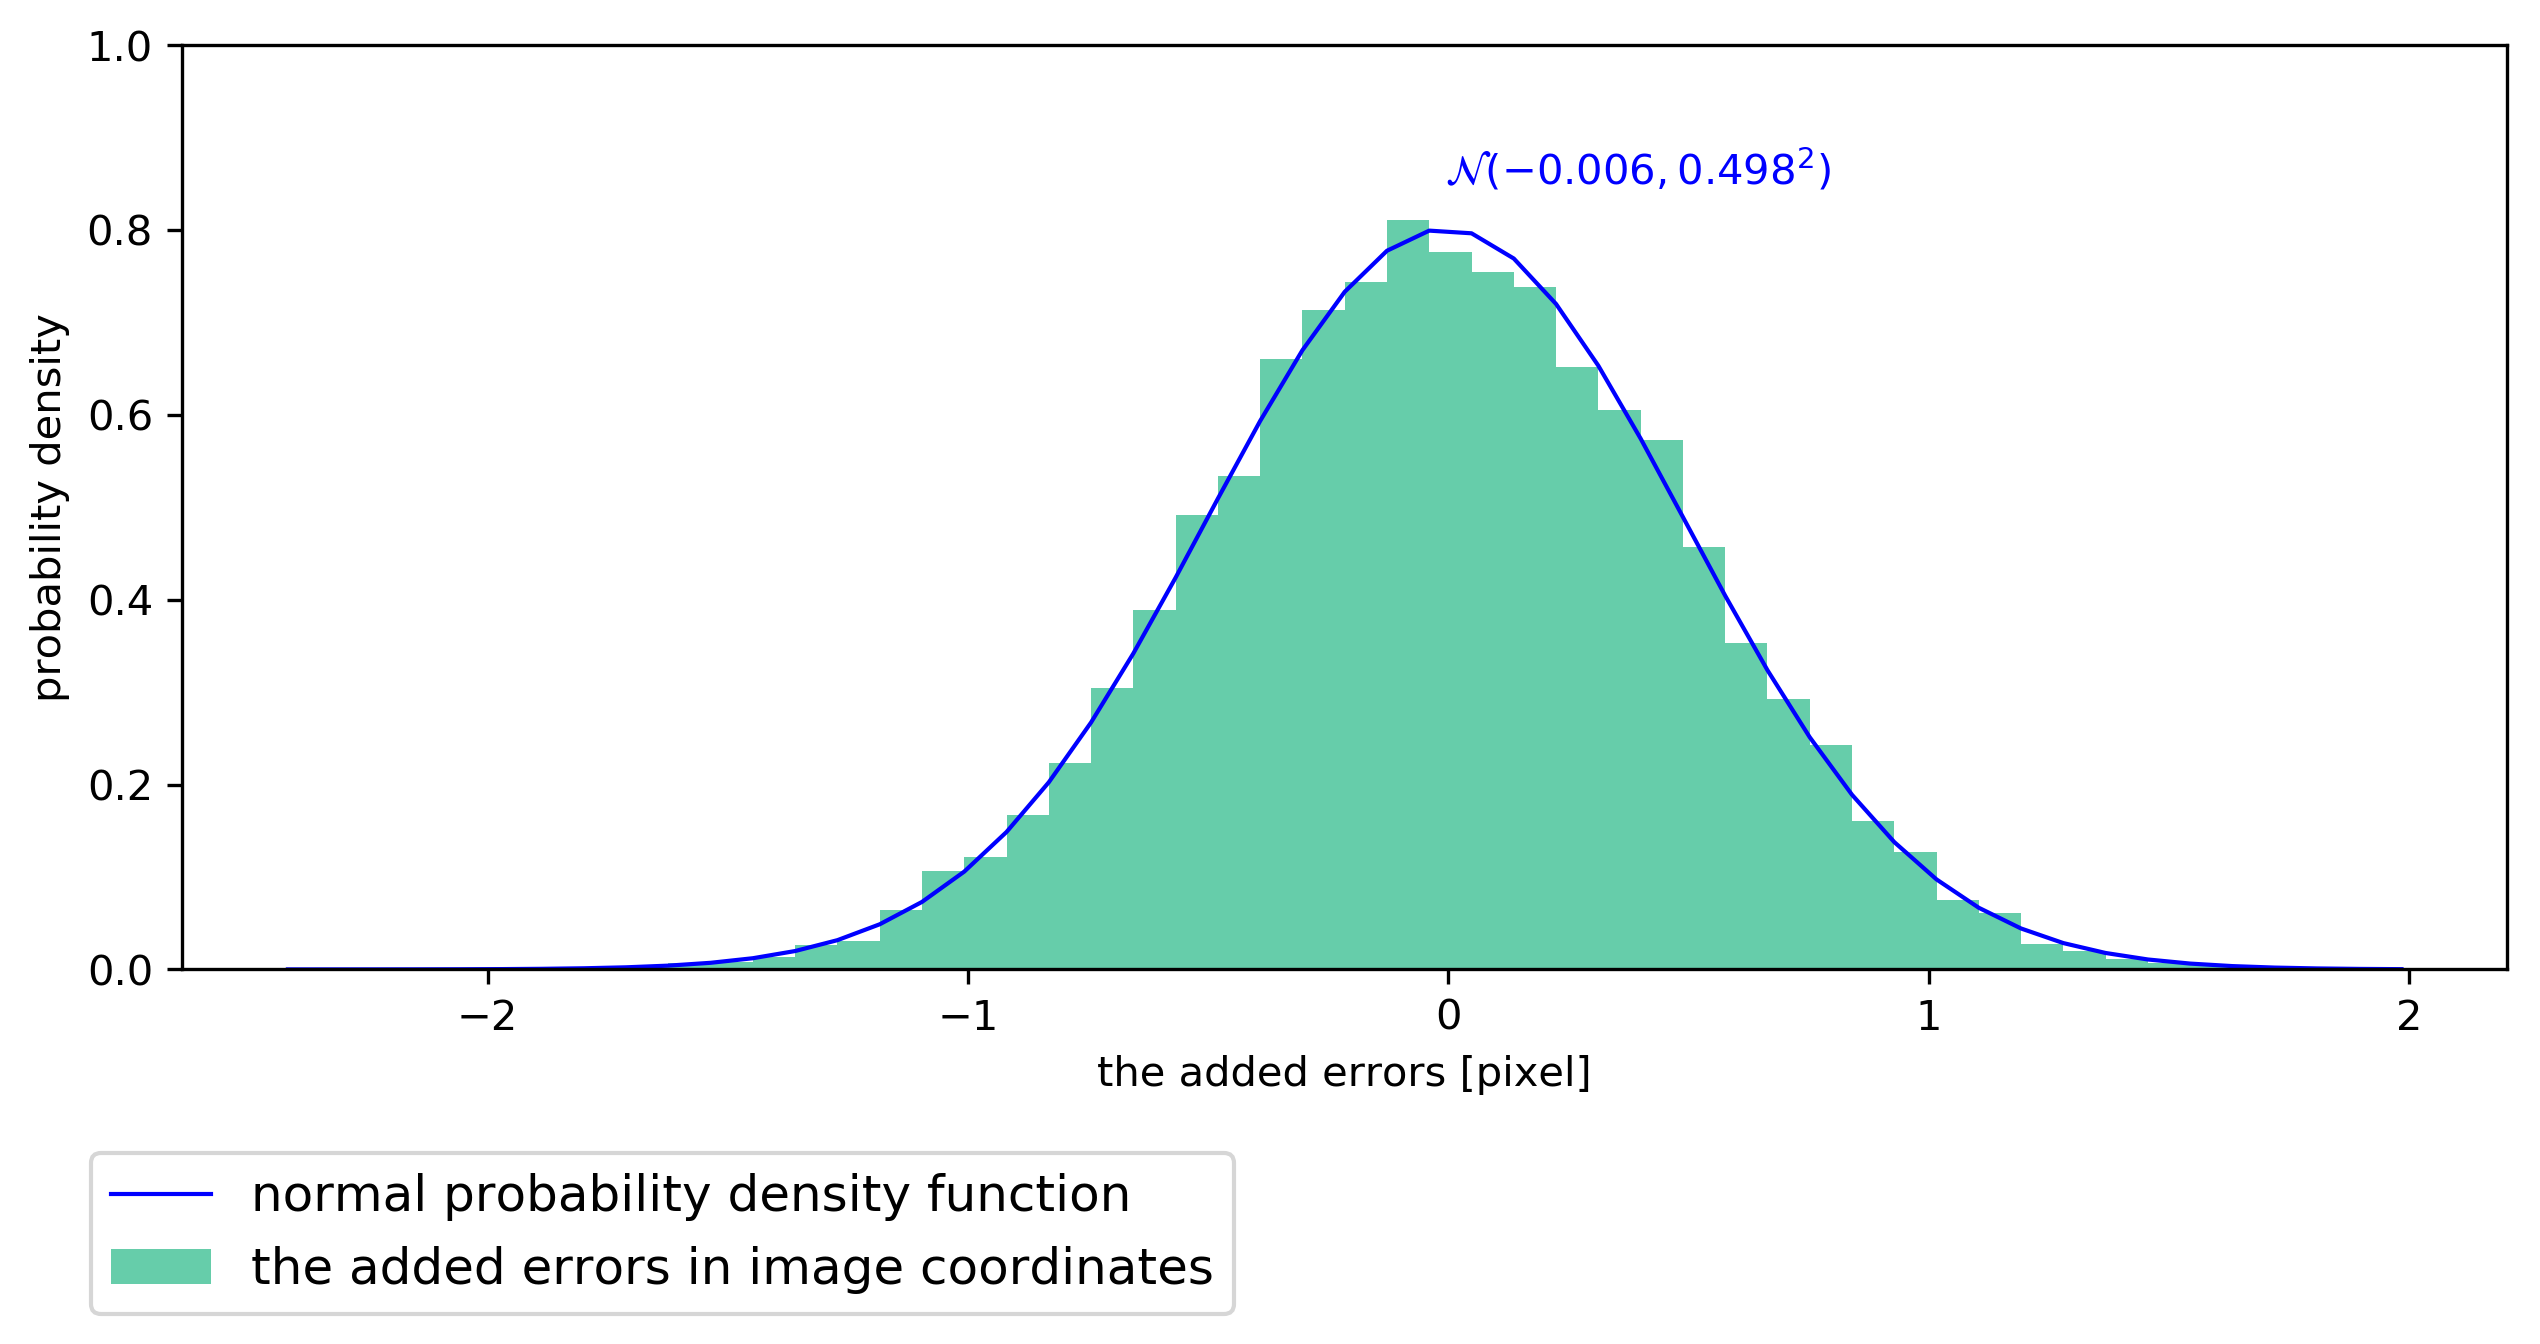
\includegraphics[width=0.8\textwidth]{Simu_errorhist_1.png}
  \caption{\small The added Gaussian random noise in the observations.}
  \label{fig:noise}
\end{figure}

\paragraph{The approximate line segment in object space}
The initial estimates for non-linear LS adjustment is generated by projecting the observed line segments in image space onto the DSM.

\clearpage

\subsection{Simulation Result}
\label{subsec:simuresult}

%%% analysis on measurements:
% 1.residuals distribution: histogram (fit line: mean, standard deviation)
% 2.normal distribution? systematic error exist? statistical test
%   or
%   standard deviation small enough? statistical test


%%% analysis on the unknowns:
\cref{fig:Simu3D_2} shows the reconstructed and the true line segments in UTM coordinate system (in Zone 32N). The distances from the reconstructed line nodes to the true line segment are collected, resulting in sample size of $18$. The sample mean is $0.008$ [meter] and the sample variance is $0.101$ [meter]. % This sampling procedure is assumed to be independent and random.%??? (t test assumptions)

For such small sample size data, a two-tailed t-test is adopted to test if the population mean significantly not equals zero, i.e. \textbf{if the reconstructed line segments are significantly far from the true line segments}. Null hypothesis ($H_0$) and (two-tailed) alternative hypothesis ($H_A$) are stated as:
\begin{equation*}
\begin{split}
H_0: \mu=0\\
H_A: \mu\neq0
\end{split}
\end{equation*}

A significance level $\alpha=0.05$ is selected, with degree of freedom being $18-1=17$, the two-tailed t-table value $T_{(0.975,17)}$ is
\begin{equation*}
T_{(0.975,17)}=2.110
\end{equation*}
which leads to the decision rule: if test statistic $T_{obs}$ is less than $-T_{(0.975,17)}=-2.110$ or greater than $T_{(0.975,17)}=2.110$, reject the null hypothesis.

With the sample mean $\overline{x}=0.008$,
the proposed population mean $\mu_0=0$,
the sample standard deviation $\sigma=0.101$,
and sample size $n=18$, the test statistic for One Sample T Test has the calculated value:
\begin{equation*}
T_{obs} = \frac{\overline{x}-\mu_0}{\sigma/\sqrt{n}}=\frac{0.008-0}{0.101/\sqrt{18}}\approx0.34
\end{equation*}
which is neither less than $-T_{(0.975,17)}=-2.110$ nor greater than $T_{(0.975,8)}=2.110$, i.e. not in the rejection region. As a result, we fail to reject the null hypothesis. In other words, \textbf{we are not able to claim that the reconstructed line is significantly far away from the true line}. This indicates that \textbf{the derived non-linear LS adjustment model for 3D reconstruction is correct}.


\begin{figure}
  \centering
  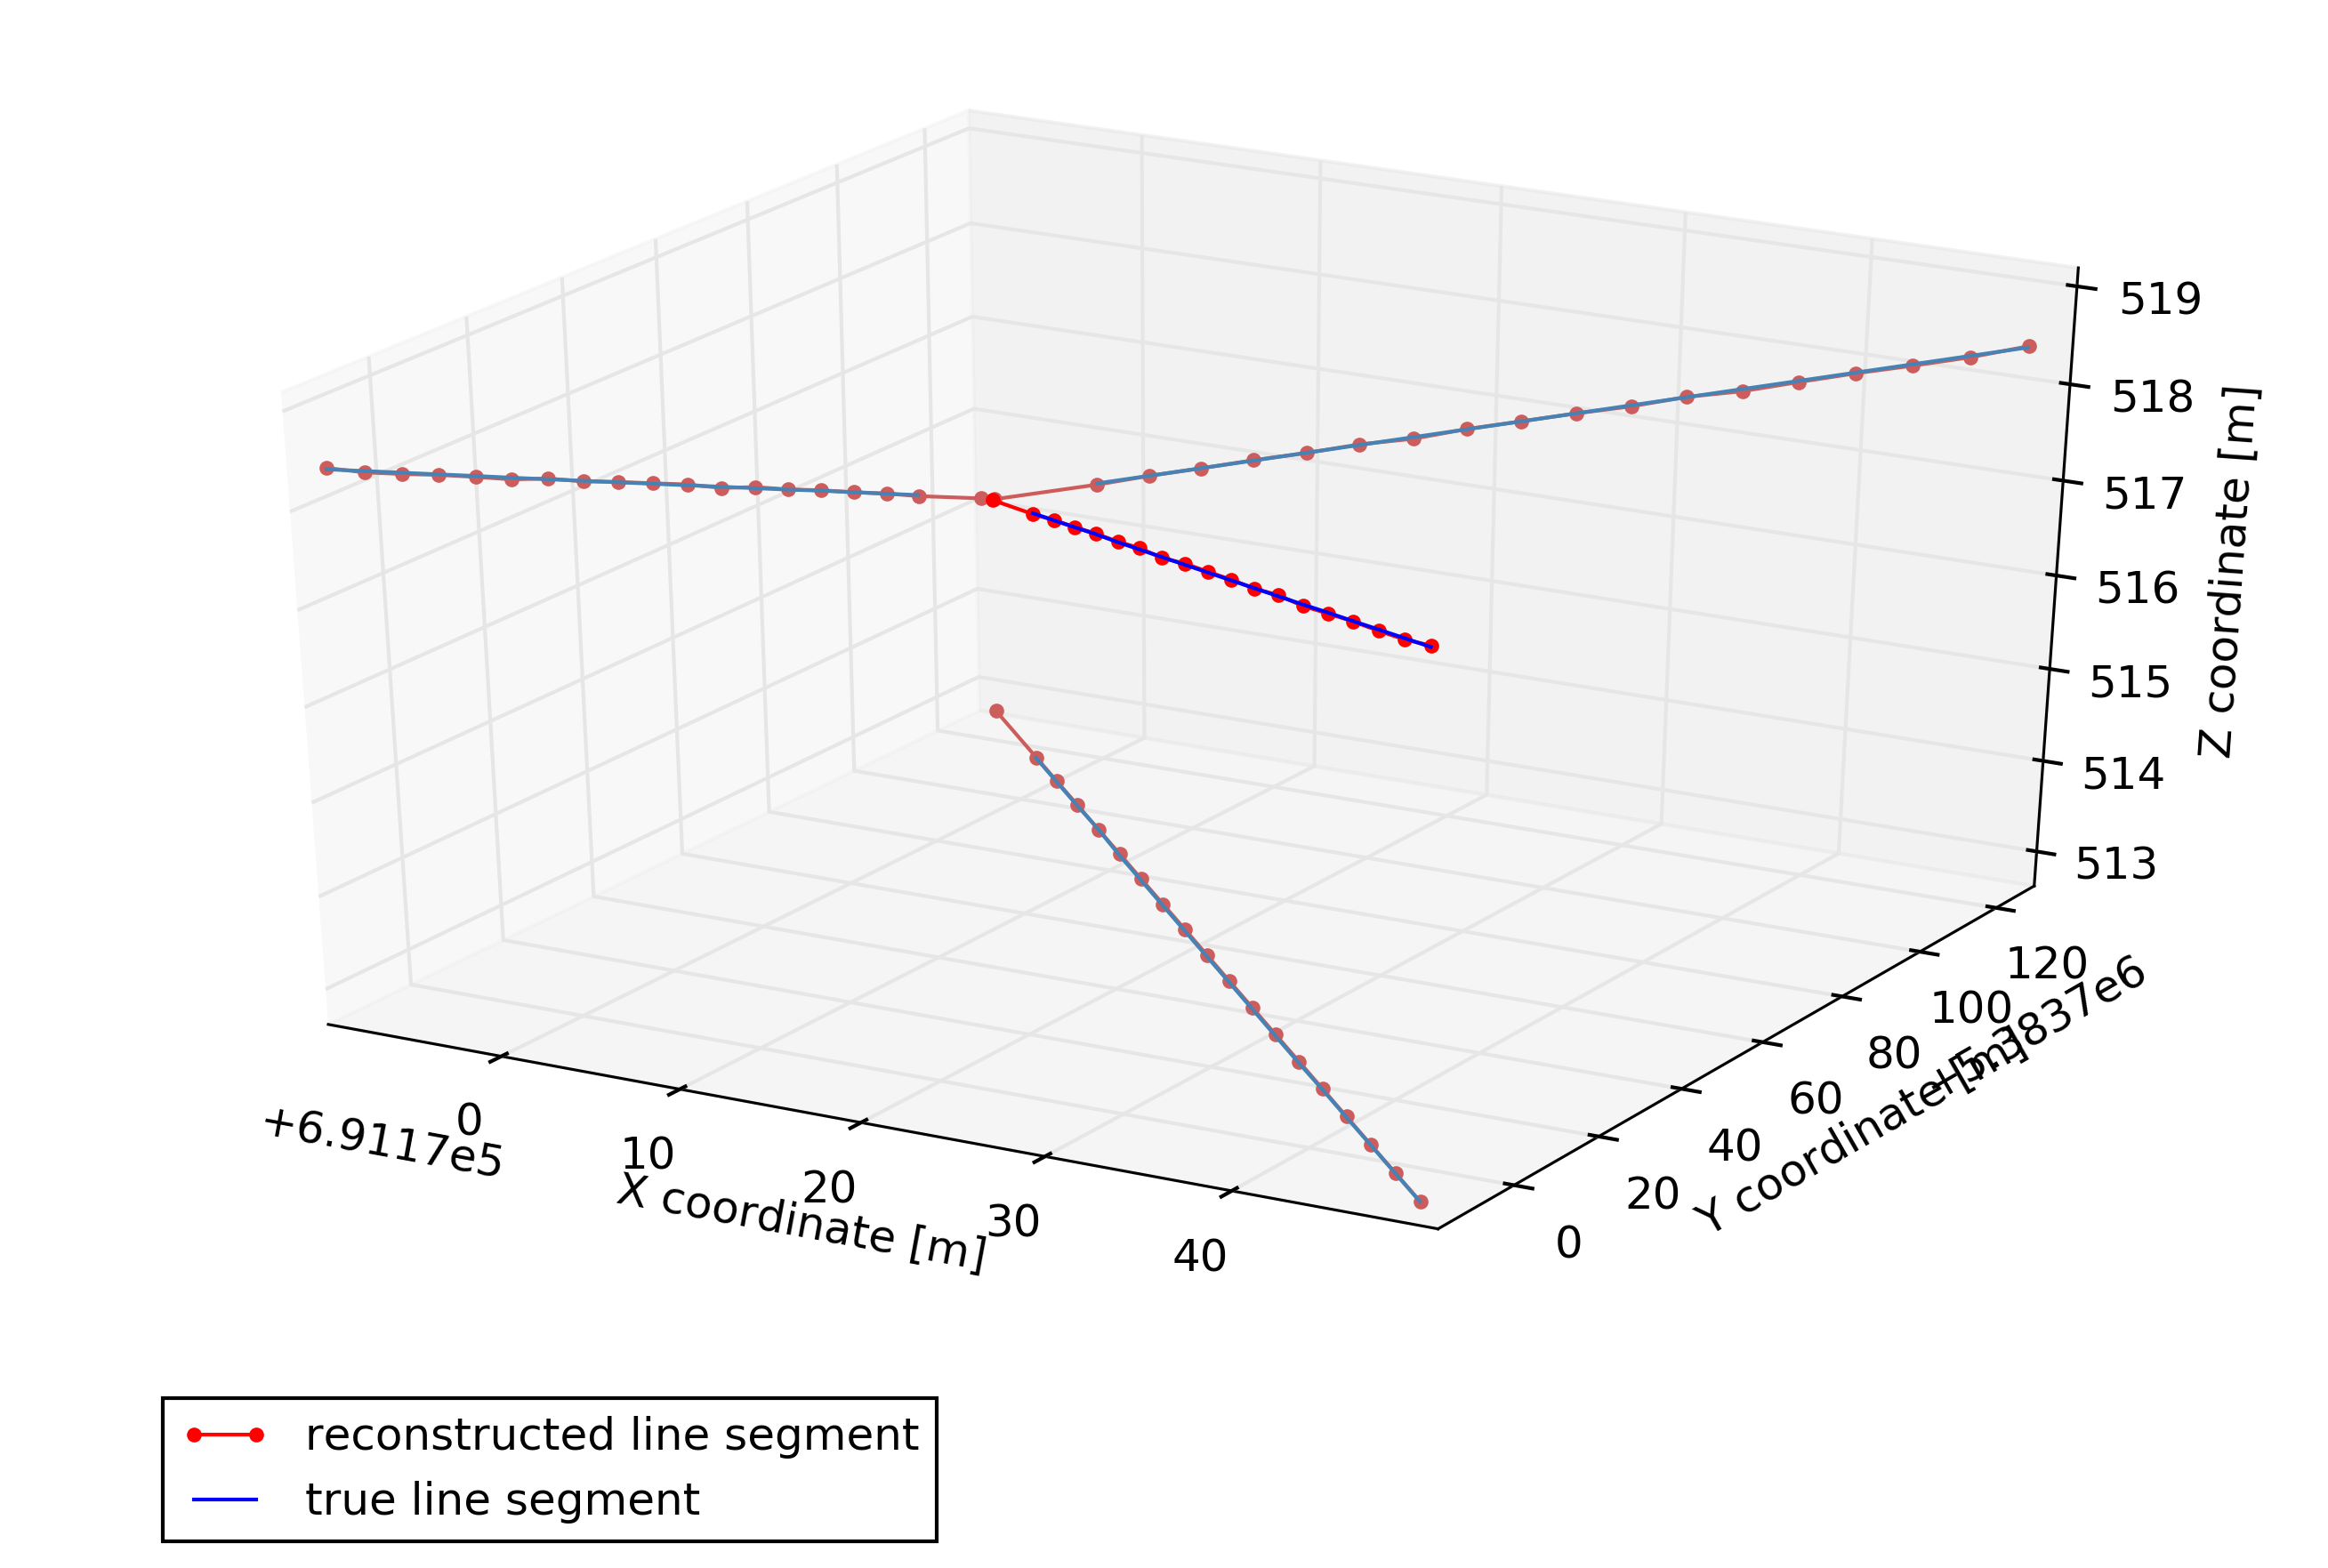
\includegraphics[width=\textwidth]{Simu_3D_2.png} %%% 換,字重疊。
  \caption{\small The reconstructed line segments and the true line segments in UTM coordinate system (in Zone 32N).}
  \label{fig:Simu3D_2}
%  \vspace{1cm}
%  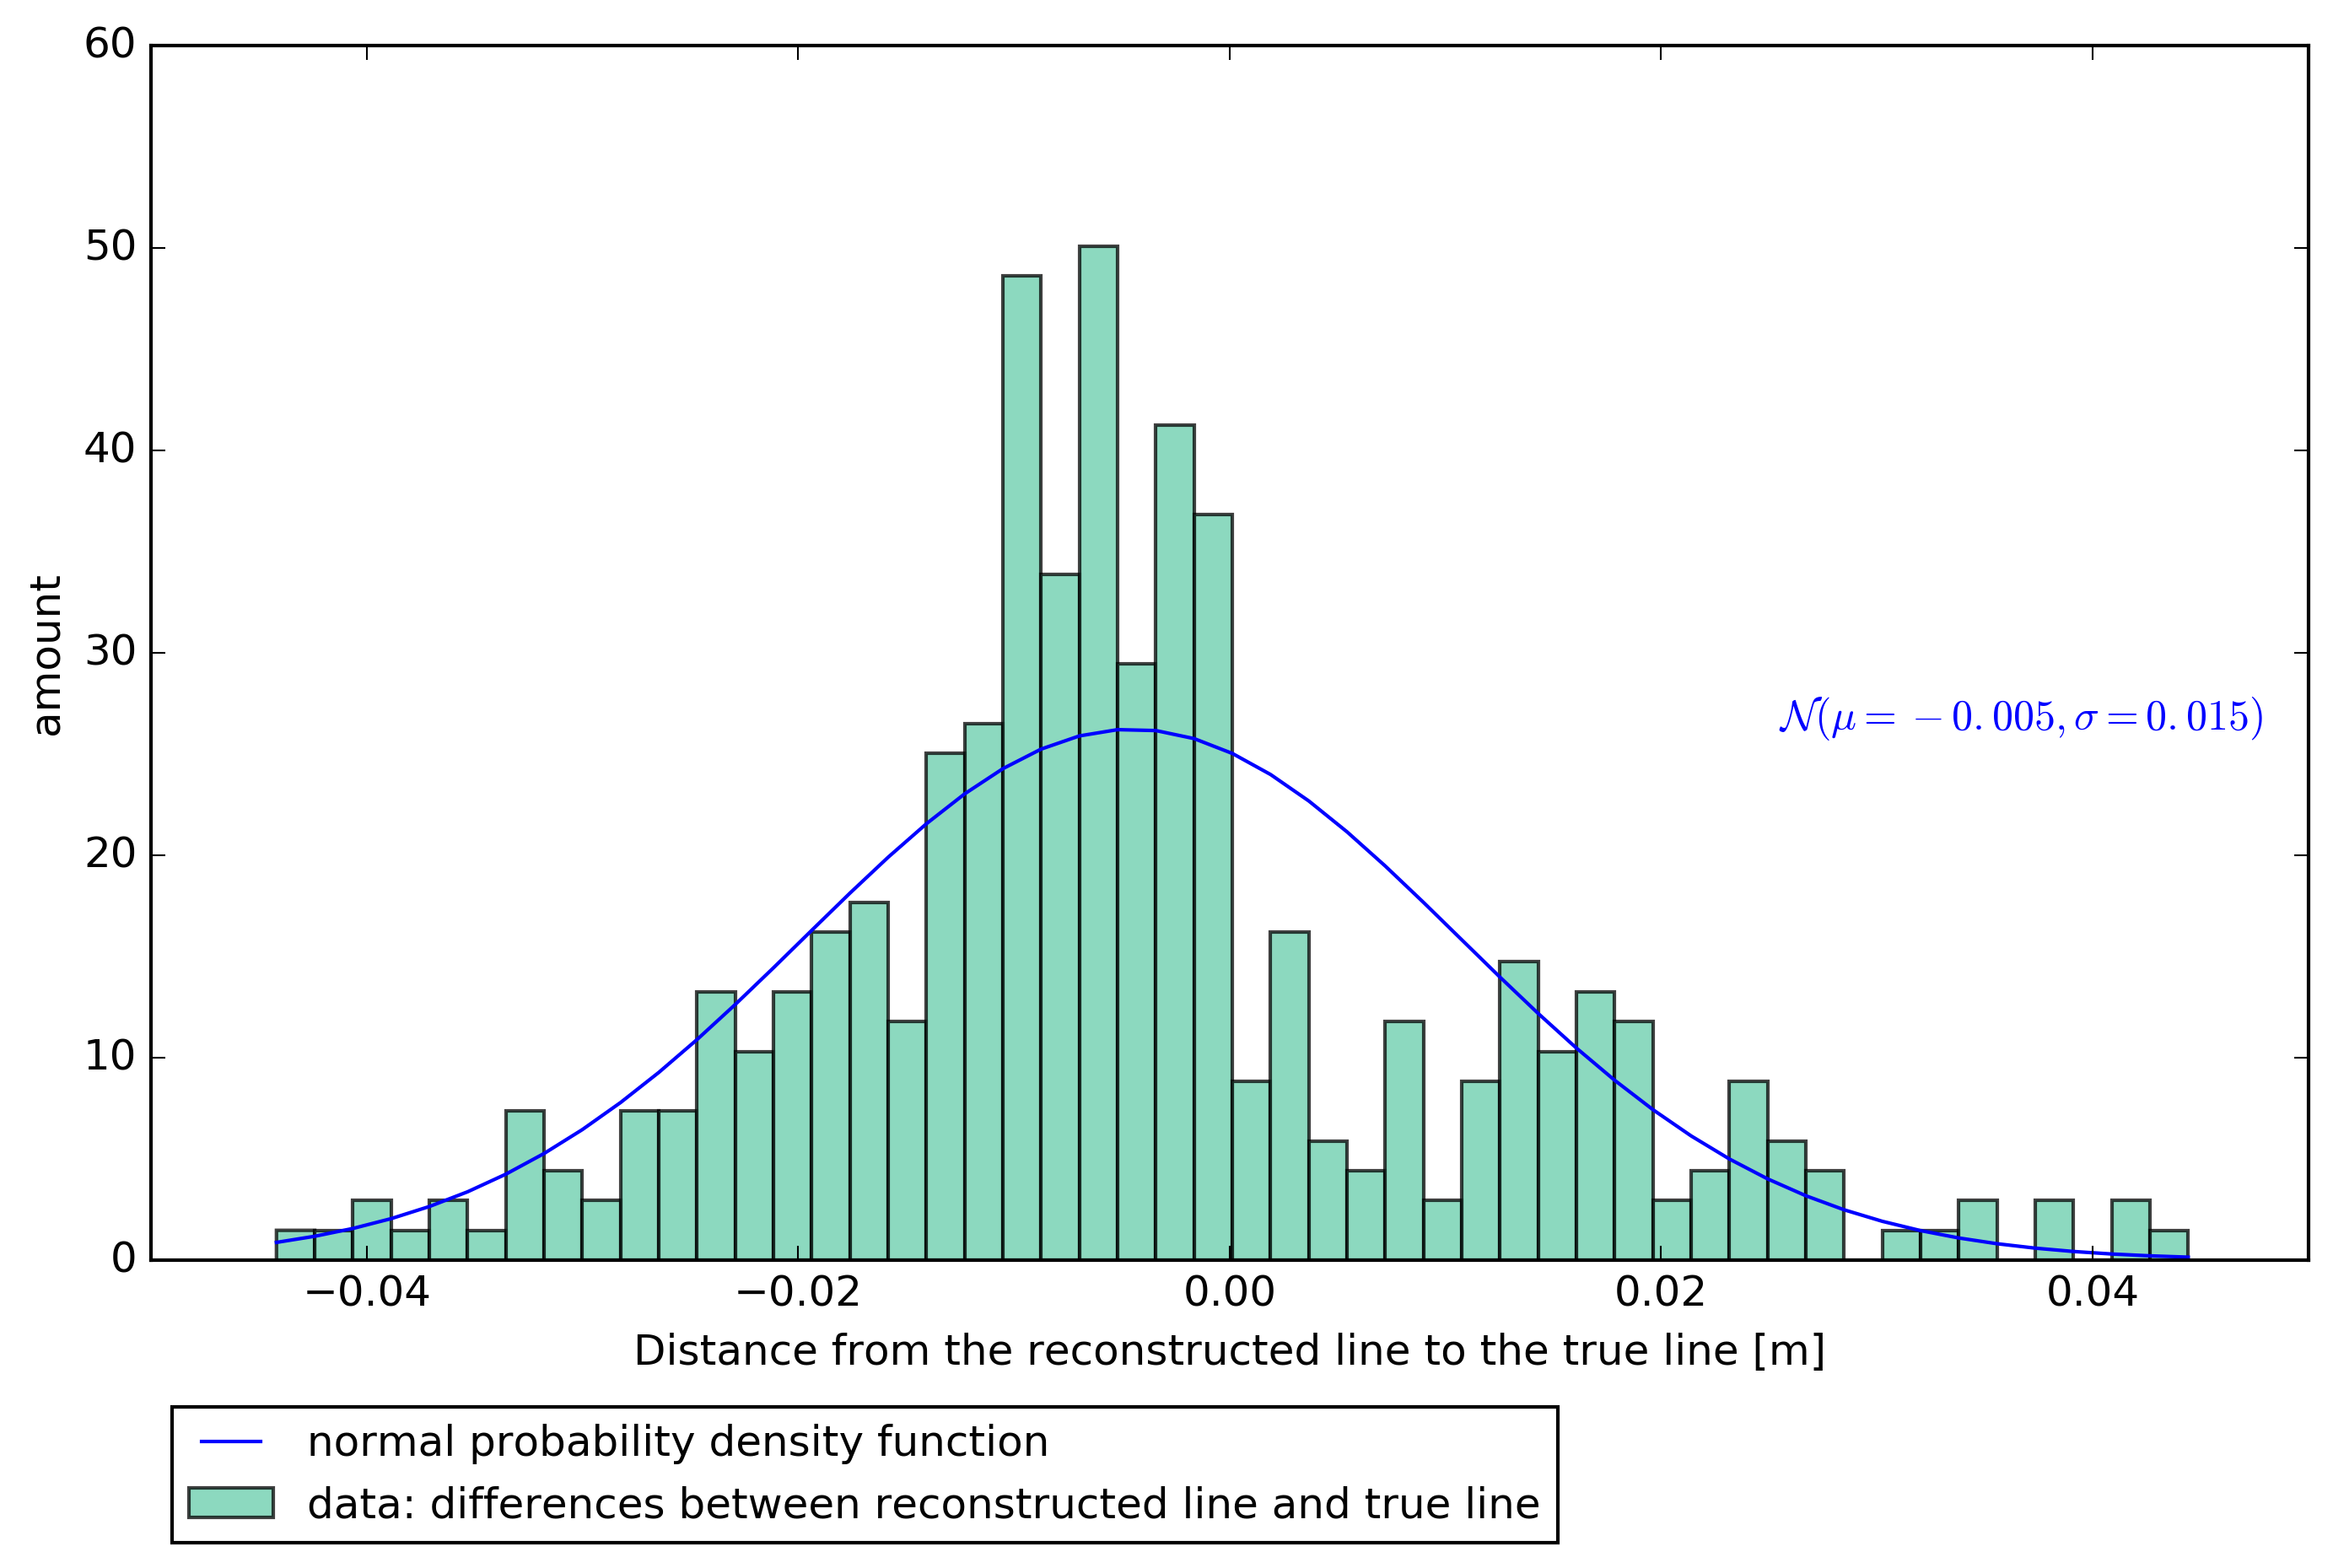
\includegraphics[width=0.8\textwidth]{Simu_hist_2.png}
%  \caption{\small Histogram of the distances between the reconstructed line and the true line.}
%  \label{fig:SimuHist_2}
\end{figure}

\clearpage

\cref{fig:Simu3D_1} shows the reconstructed line segments and the DSM profile which serves as the initial approximation for non-linear LS adjustment, in UTM coordinate system (in Zone 32N). The maximum distance between them is 1.97 meter, mainly in Z-direction. This tells that \textbf{the reconstruction model is able to refine the initial approximation with at least 2 meters bias in Z-direction}.


%The distances from the reconstructed line segment to the DSM profile are plotted into histogram in \cref{fig:SimuHist_1}. They are collected along the reconstructed line segments with 0.2 meter spacing (considering the DSM grid of 0.2 meter), resulting in sample size of $381$. The sample mean is $-0.029$ [meter] and the sample variance is $0.083$ [meter]. % This sampling procedure is assumed to be independent and random.%??? and normal distributed (Z test assumptions)

%In order to know \textbf{if the mean distance from the reconstructed line segments to the DSM profile is significantly non-zero}, a two-tailed Z-test is adopted for such big sample size cases. Null hypothesis ($H_0$) and (two-tailed) alternative hypothesis ($H_A$) are stated as:
%\begin{equation*}
%\begin{split}
%H_0: \mu=0\\
%H_A: \mu\neq0
%\end{split}
%\end{equation*}

%A significance level $\alpha=0.05$ is selected, which is $0.025$ on each tail of the population, i.e. the area in body is $0.975$ out of 100\%. The corresponding z-score is:
%\begin{equation*}
%Z_{0.975}=1.96
%\end{equation*}
%which leads to the decision rule: if $Z_{obs}$ is less than $-1.96$ or greater than $1.96$, reject the null hypothesis.

%With the sample mean $\overline{x}=-0.029$,
%the proposed population mean $\mu_0=0$,
%the sample standard deviation $\sigma=0.083$,
%and sample size $n=381$, the test statistic for a One Sample Z Test has a calculated value:
%\begin{equation*}
%Z_{obs} = \frac{\overline{x}-\mu_0}{\sigma/\sqrt{n}}=\frac{-0.029-0}{0.083/\sqrt{381}}\approx-6.82
%\end{equation*}

%As the test statistic $Z_{obs}\approx-6.82$ is less than $-Z_{0.975}=-1.96$, i.e. in the rejection region, the null hypothesis is rejected. In other words, \textbf{with 95\% confidence we can claim that the mean distance from the reconstructed line segment to the DSM profile is significantly non-zero}. This phenomenon is as expected, as mentioned in sec:DSM???. 


\begin{figure}
  \centering
  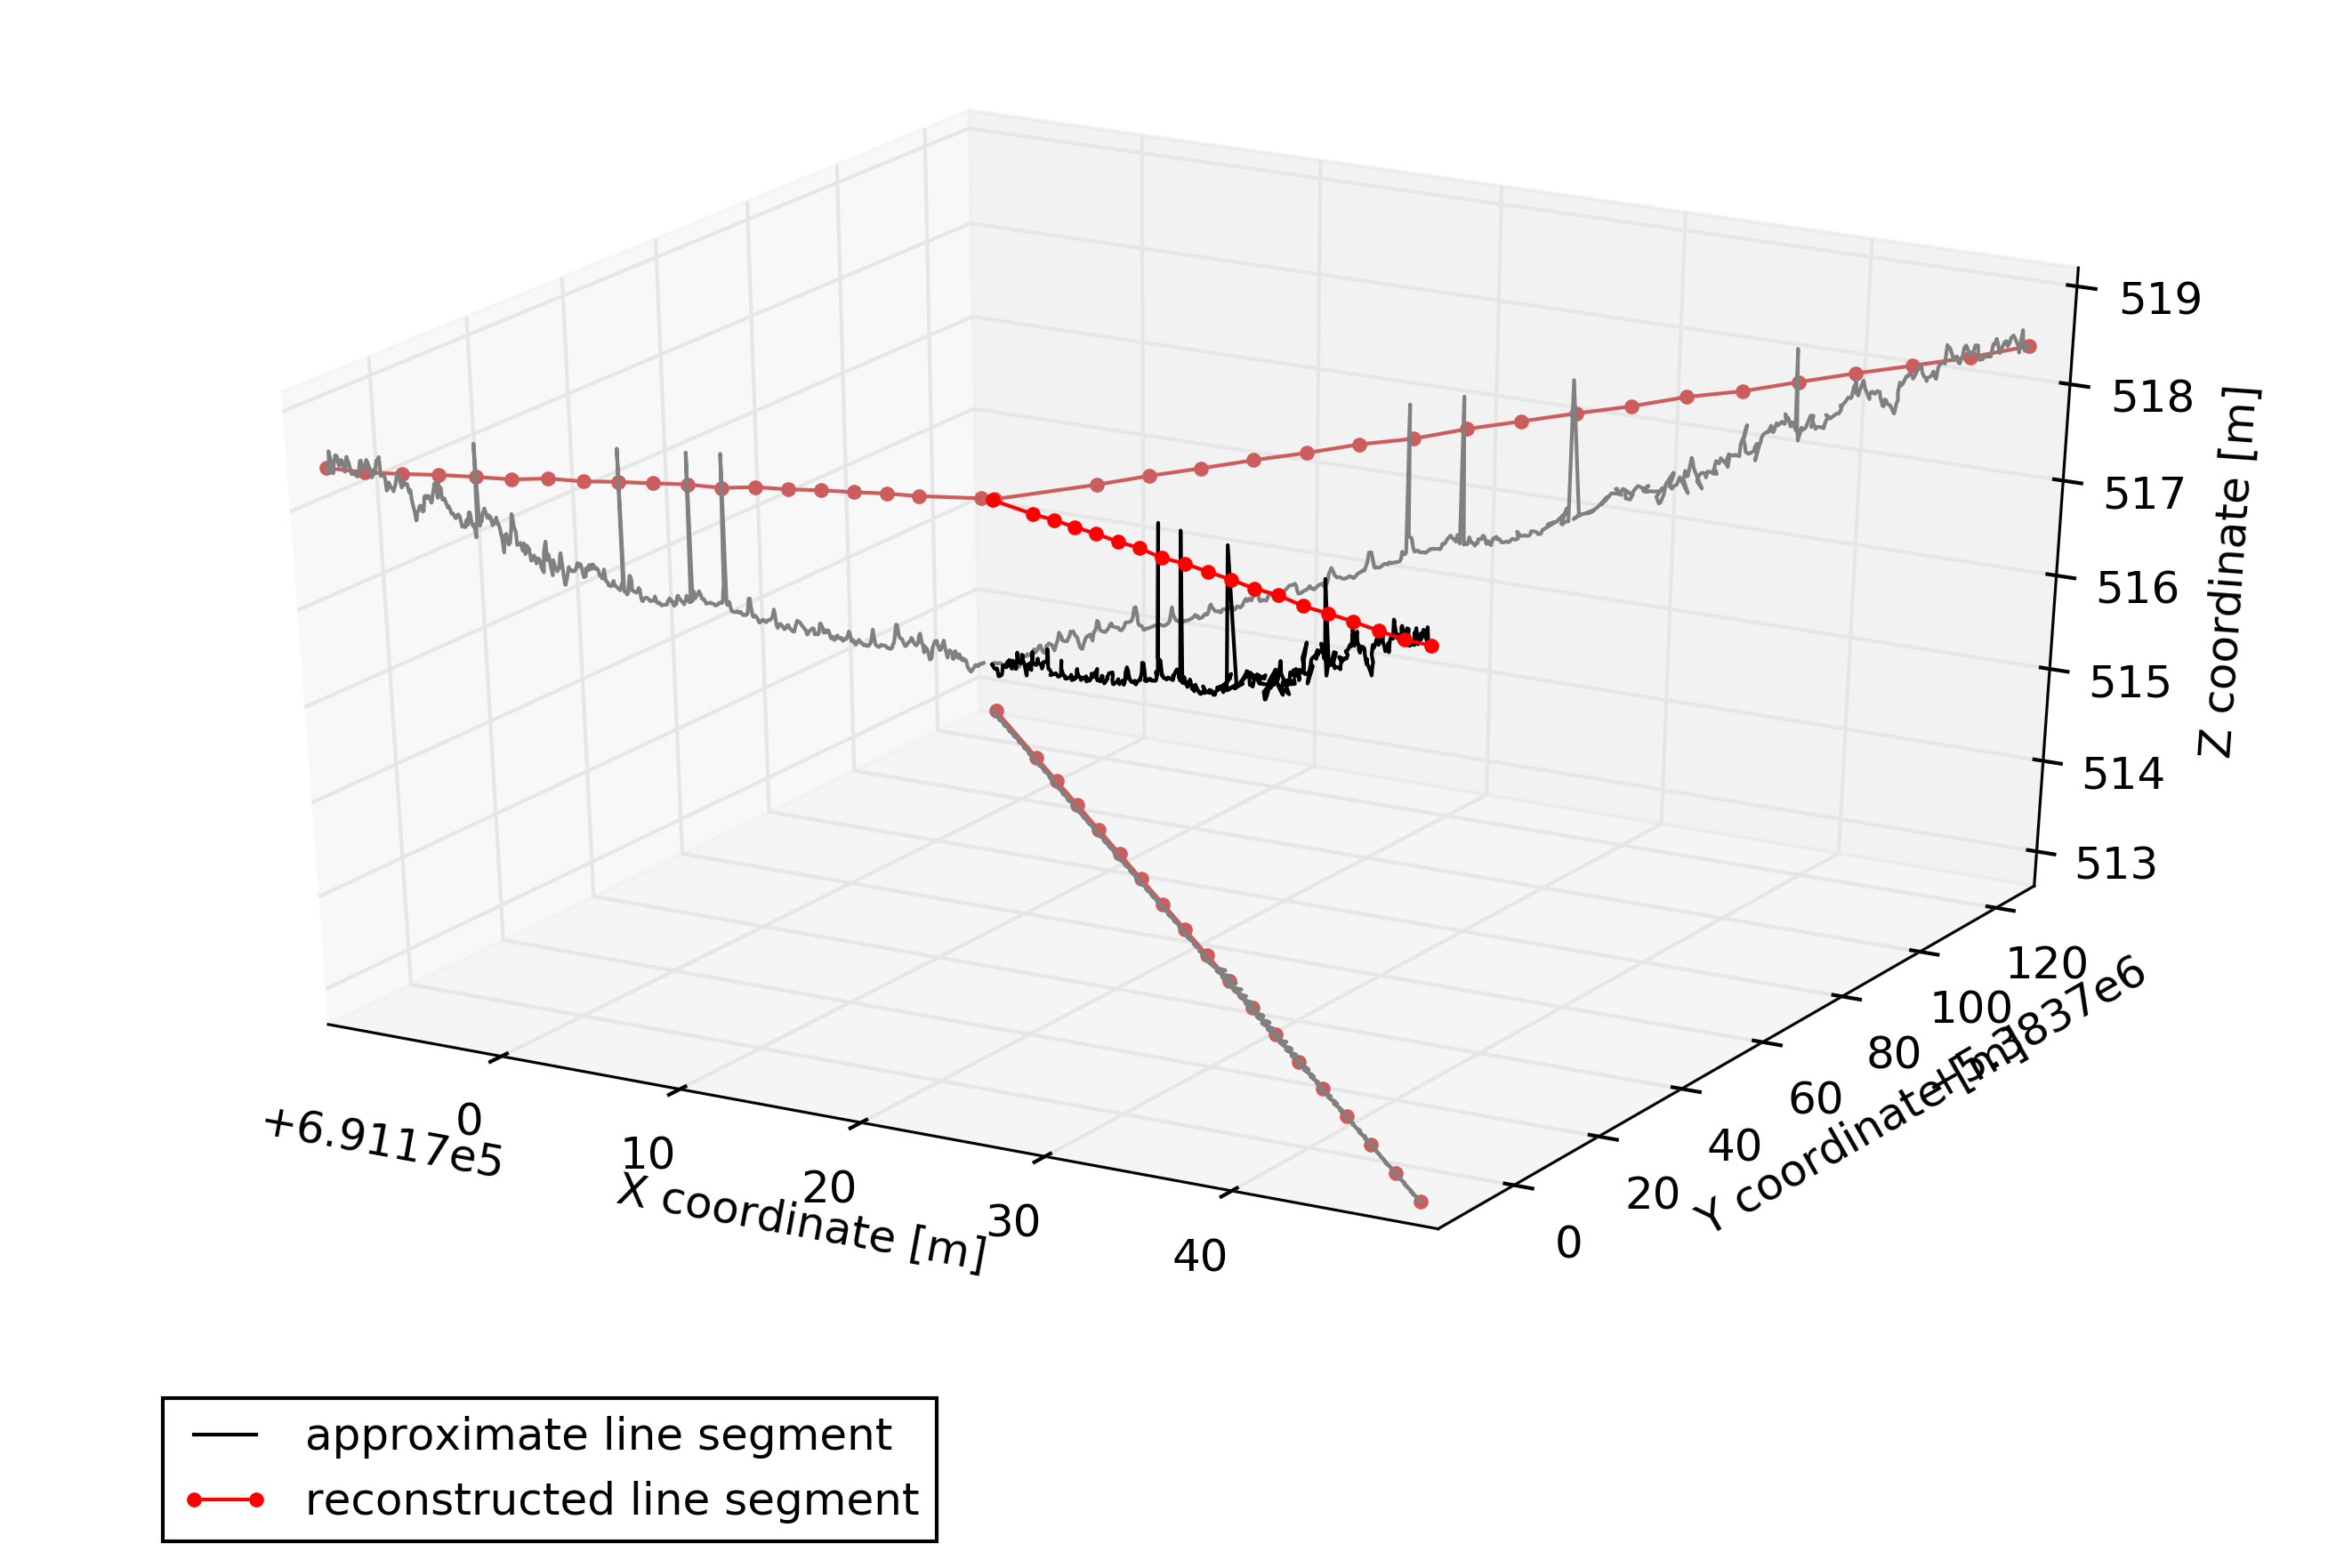
\includegraphics[width=\textwidth]{Simu_3D_1.png}
  \caption{\small The reconstructed line segments and the unrefined DSM profile in UTM coordinate system (in Zone 32N).}
  \label{fig:Simu3D_1}
%  \vspace{1cm}
%  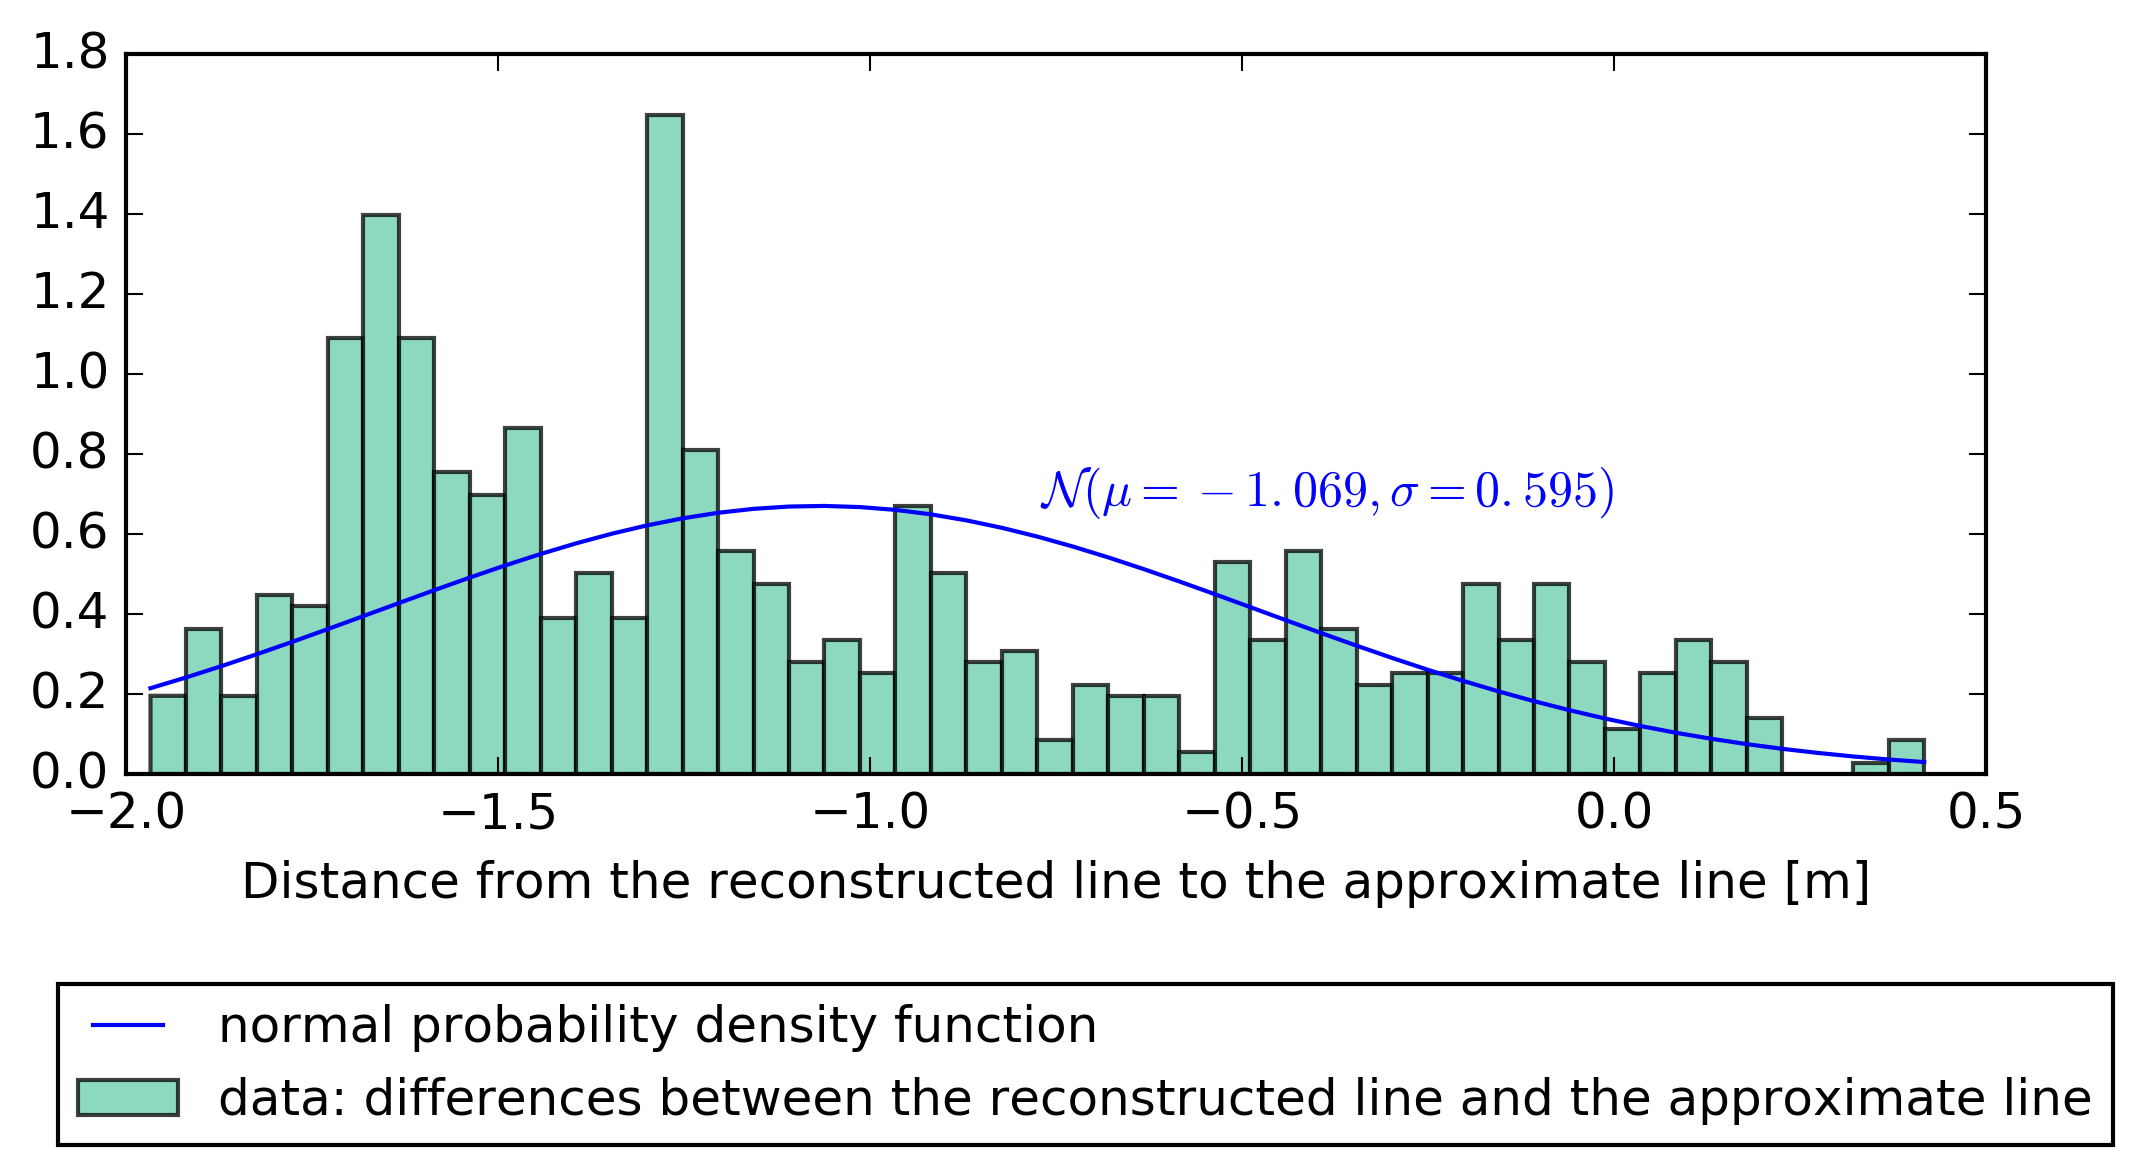
\includegraphics[width=\textwidth]{Simu_hist_1.png}
%  \caption{\small Histogram of the distances between the reconstructed line and the unrefined DSM profile.}
%  \label{fig:SimuHist_1}
\end{figure}

\cref{fig:SimuImgNum_1} shows the amount of images (different views), the redundancies, the posterior standard deviation and the height of the reconstructed line nodes. Each segment is an independent LS adjustment process.

%The redundancies increase with more covering images.
%The posterior standard deviation
%\begin{equation*}
%\hat{\sigma}_0=\sqrt{\dfrac{\sum\hat{e}^\mathsf{T}\hat{e}}{redundancy}}
%\end{equation*}
%reflects the measurement quality.
%posterior standard deviation appears to have no obvious correlation with the amount of images.  Unless the included measurements

\begin{figure}
  \centering
  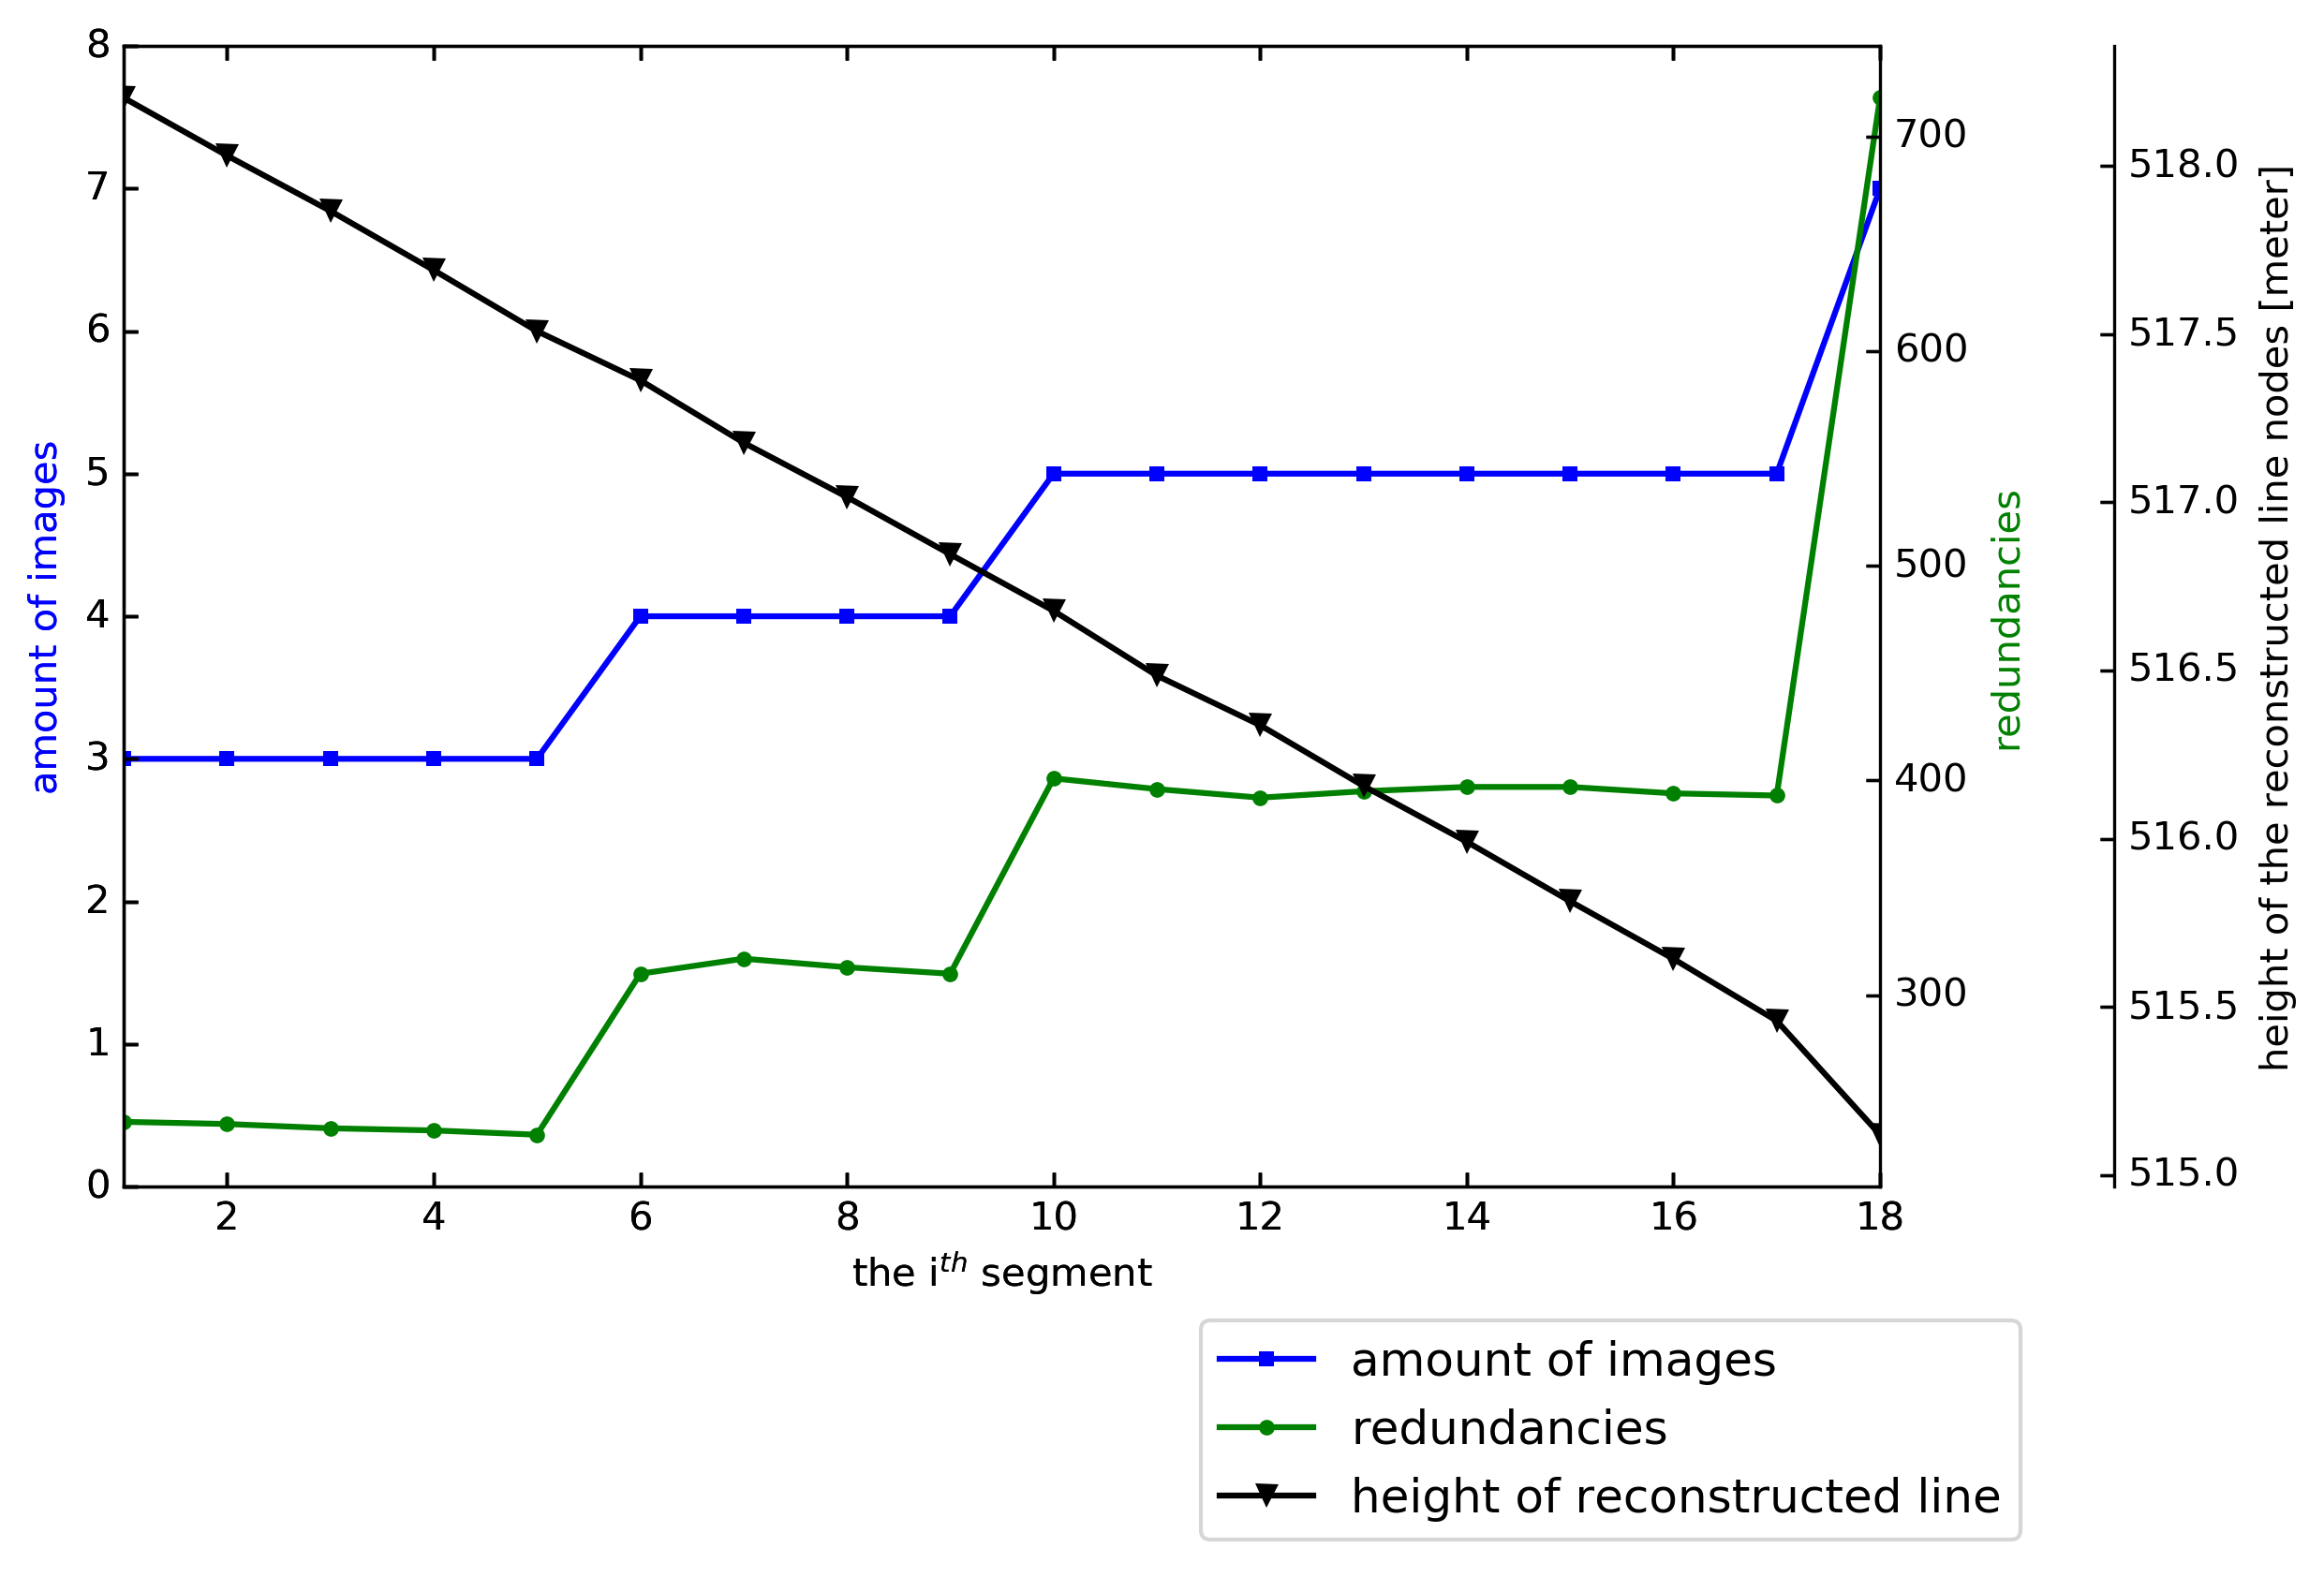
\includegraphics[width=\textwidth]{Simu_ImgNum.png}
  \caption{\small XXX.}
  \label{fig:SimuImgNum_1}
\end{figure}

From \cref{fig:SimuSigmaxx} it can be seen that the estimated parameters in horizontal direction, i.e. $\hat{X}$ and $\hat{Y}$, have smaller priori variances values $\sqrt{\sigma_{\hat{X}}^2+\hat{\sigma}_{\hat{Y}}^2}$ with more covering images.

\begin{figure}
  \centering
  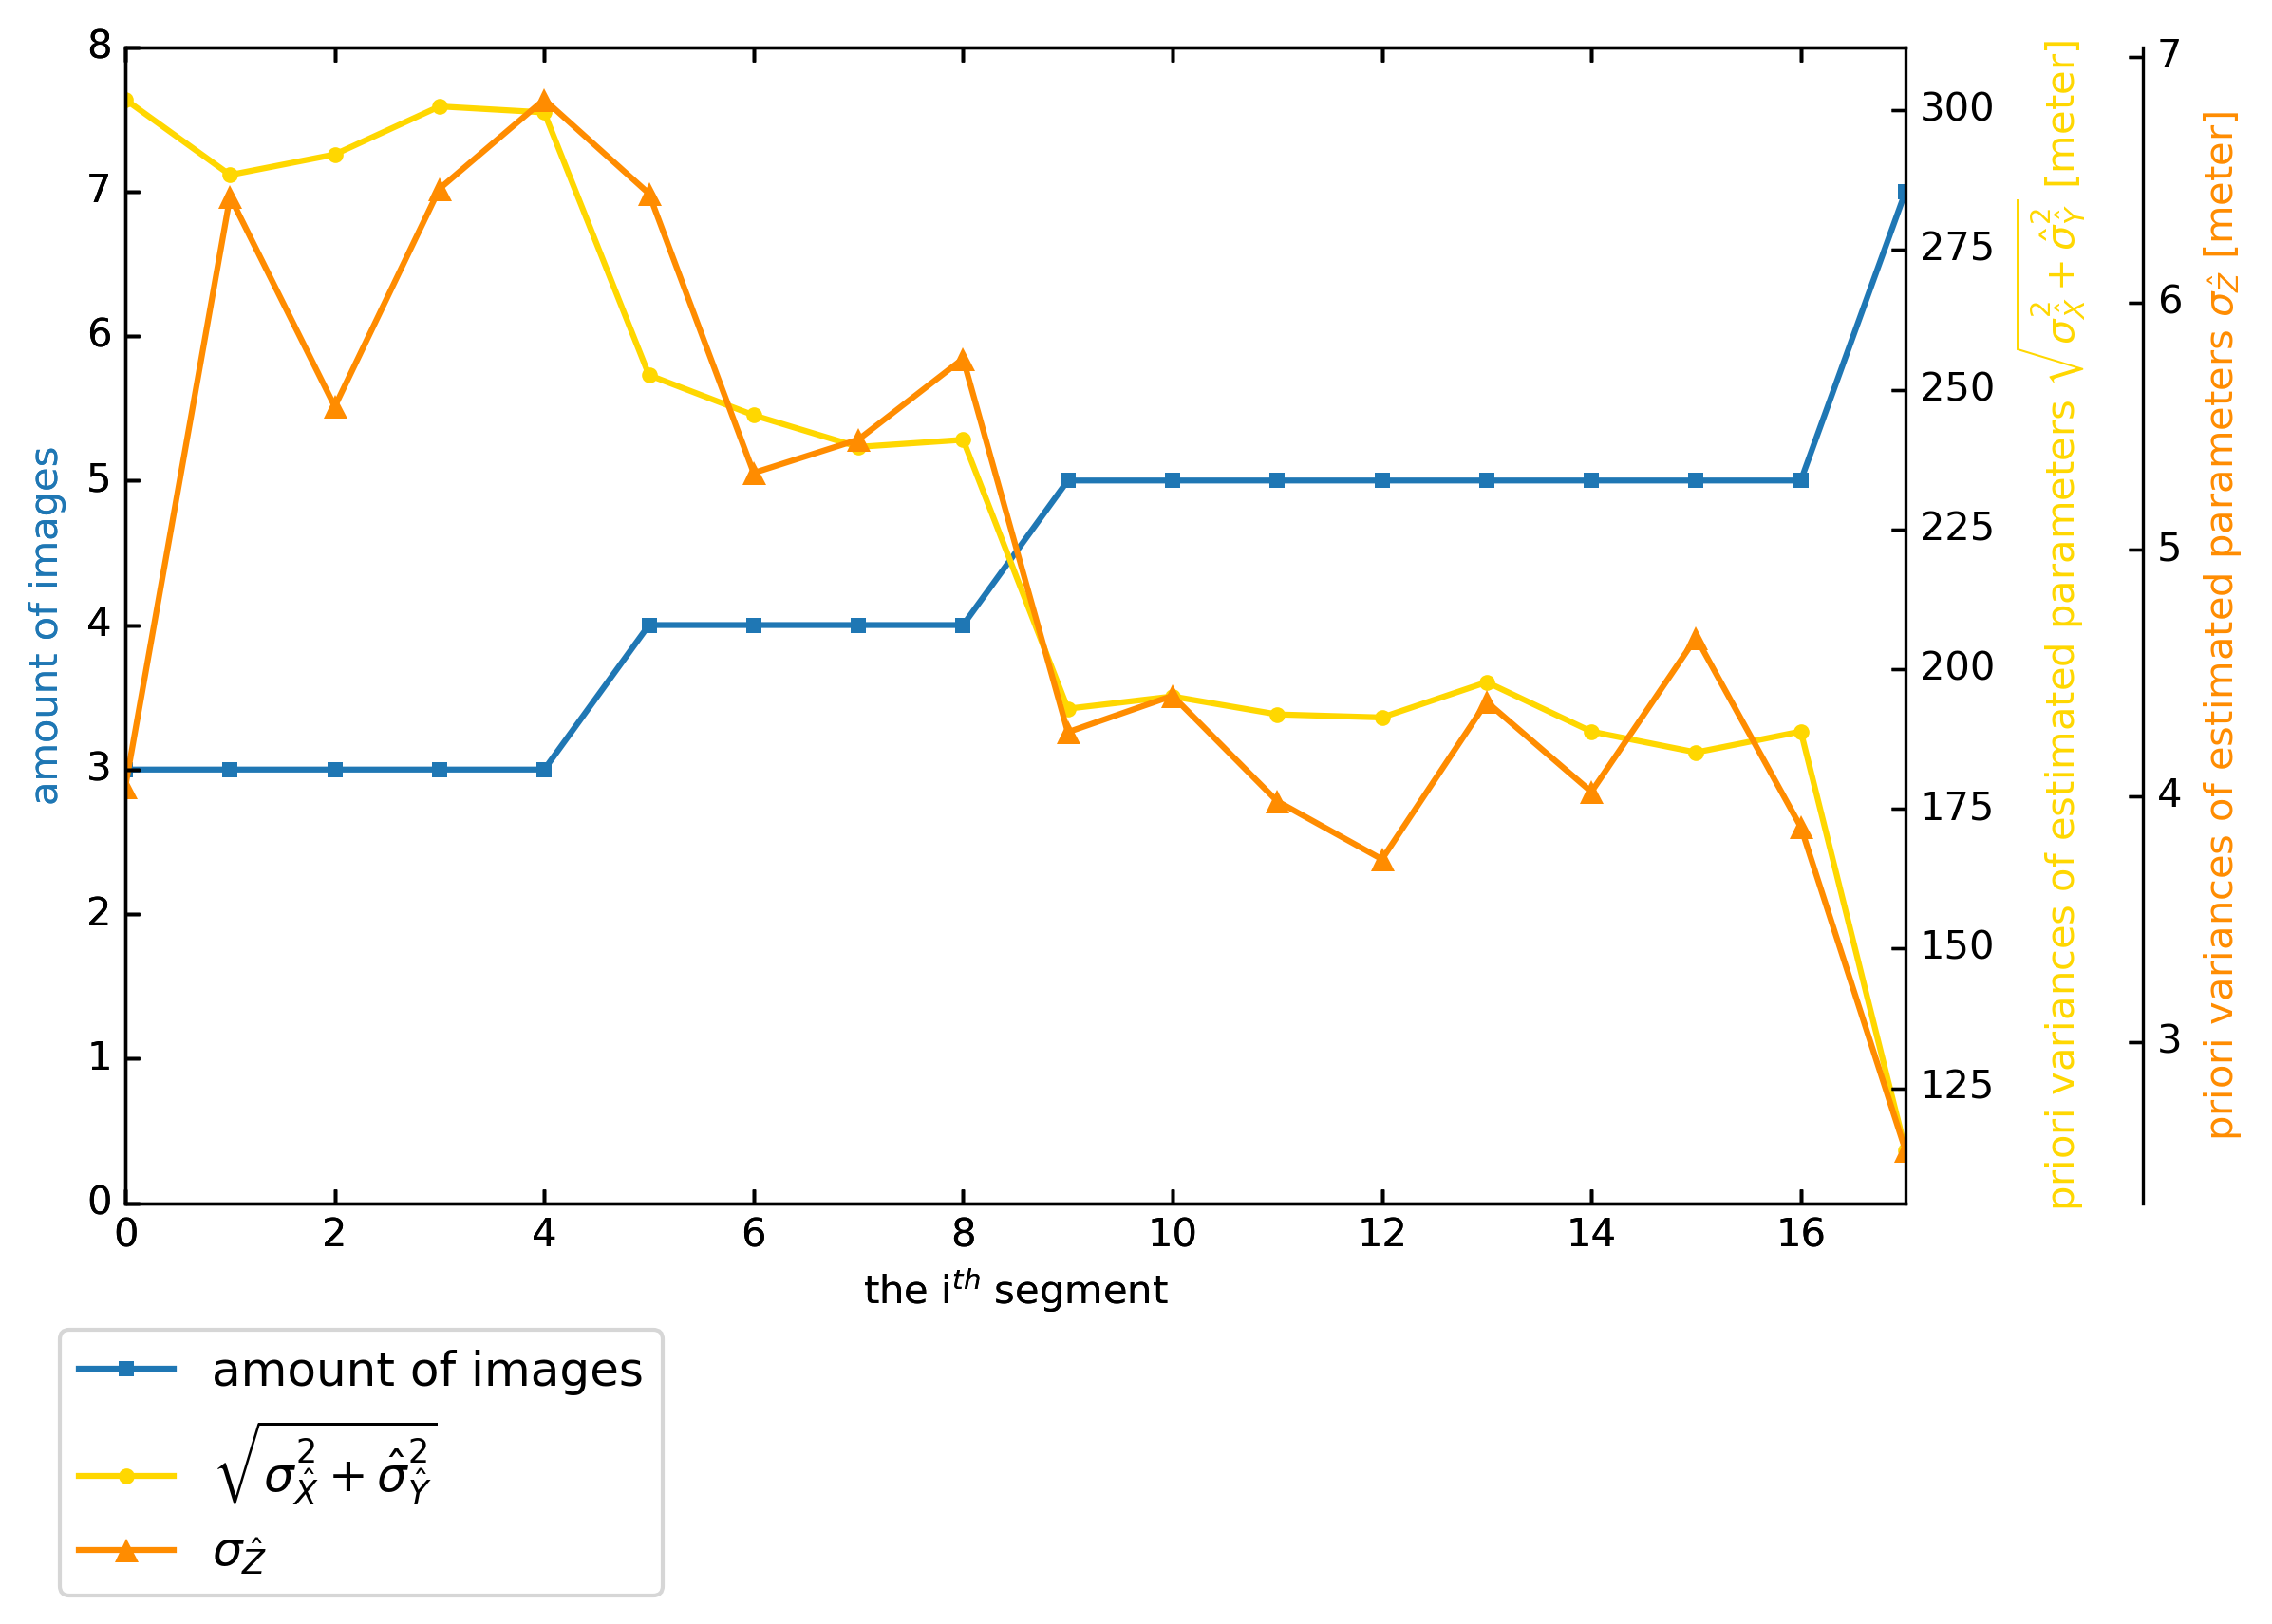
\includegraphics[width=\textwidth]{Simu_XY_Z.png}
  \caption{\small The relation between the variances of the estimated parameters and the amount of images.}
  \label{fig:SimuSigmaxx}
\end{figure}





\clearpage


%\subsection{Simulation Result: case 2}
%\label{subsec:simuresult-2}
%analysis on measurements:
% 1.residuals distribution: histogram (fit line: mean, standard deviation)
% 2.normal distribution? systematic error exist? statistical test
% 3.as expected? (the same as the added random errors) statistical test
 
%reconstructed line vs true line (accuracy?)

%statistical test: errors small enough?




%%%%%%%%%%%%%%%%%%%%%%%%%%%%%%%%%%%%%%%%%%%%%%%%%%%%%%%%
\section{True Data}
\label{sec:truedata}

table:
%case1: Dashed Lane marking
case2: Continuous Lane marking%, two strips, multiple stereo pairs
%case3: Continuous Lane marking, two strips, two stereo pairs
%case4: Continuous Lane marking, two strips, one stereo pair
%case5: Continuous Lane marking, one strip

covering images, observations, unknowns, redundancies, 



%\subsection{True Data Result: case 1 -Dashed Lane Marking}
%\label{subsec:trueresult-1}


\subsection{True Data Result: case2 -Continuous Lane Marking}
\label{subsec:trueresult-2}

A continuous lane marking of ??? meters length is reconstructed. \cref{fig:Test3D_1} shows the reconstructed line segments and the DSM profile in UTM coordinate system (in Zone 32N). The distances from the reconstructed line segment to the DSM profile are plotted into histogram in \cref{fig:TestHist_1}. They are collected along the reconstructed line segments with 0.2 meter spacing (considering the DSM grid of 0.2 meter), resulting in sample size of $1256$. The sample mean is $-0.180$ [meter] and the sample standard deviation is $0.174$ [meter]. %This sampling procedure is assumed to be independent and random.%??? and normal distributed (Z test assumptions)

Assuming DSM height profile being significantly lower than the reconstructed line segments for more than $17$??? centimeters, a lower-tailed Z-test is adopted. Null hypothesis ($H_0$) and (one-tailed) alternative hypothesis ($H_A$) are stated as:
\begin{equation*}
\begin{split}
H_0: \mu\geq-0.170\\
H_A: \mu<-0.170
\end{split}
\end{equation*}

A significance level $\alpha=0.05$ is selected, i.e. the area in body is $0.950$ out of 100\%. The corresponding z-score is:
\begin{equation*}
Z_{0.950}=1.64
\end{equation*}
leads to the decision rule: if $Z_{obs}$ is less than $-1.64$, reject the null hypothesis.

With the sample mean $\overline{x}=-0.180$,
the proposed population mean $\mu_0=-0.170$,
the sample standard deviation $\sigma=0.174$,
and sample size $n=1256$, the test statistic for a One Sample Z Test has a calculated value:
\begin{equation*}
Z_{obs} = \frac{\overline{x}-\mu_0}{\sigma/\sqrt{n}}=\frac{-0.180-(-0.170)}{0.174/\sqrt{1256}}\approx-4.07
\end{equation*}

As the test statistic $Z_{obs}\approx-4.07$ is less than $-Z_{0.95}=-1.64$, i.e. in the rejection region, the null hypothesis is rejected. In other words, \textbf{with 95\% confidence we can claim that the DSM profile is in average, statistically significantly lower than the reconstructed line segments for more than $\mathbf{17}$ centimeters}. %This phenomenon is as expected, as mentioned in sec:DSM??? 

\begin{figure}
  \centering
  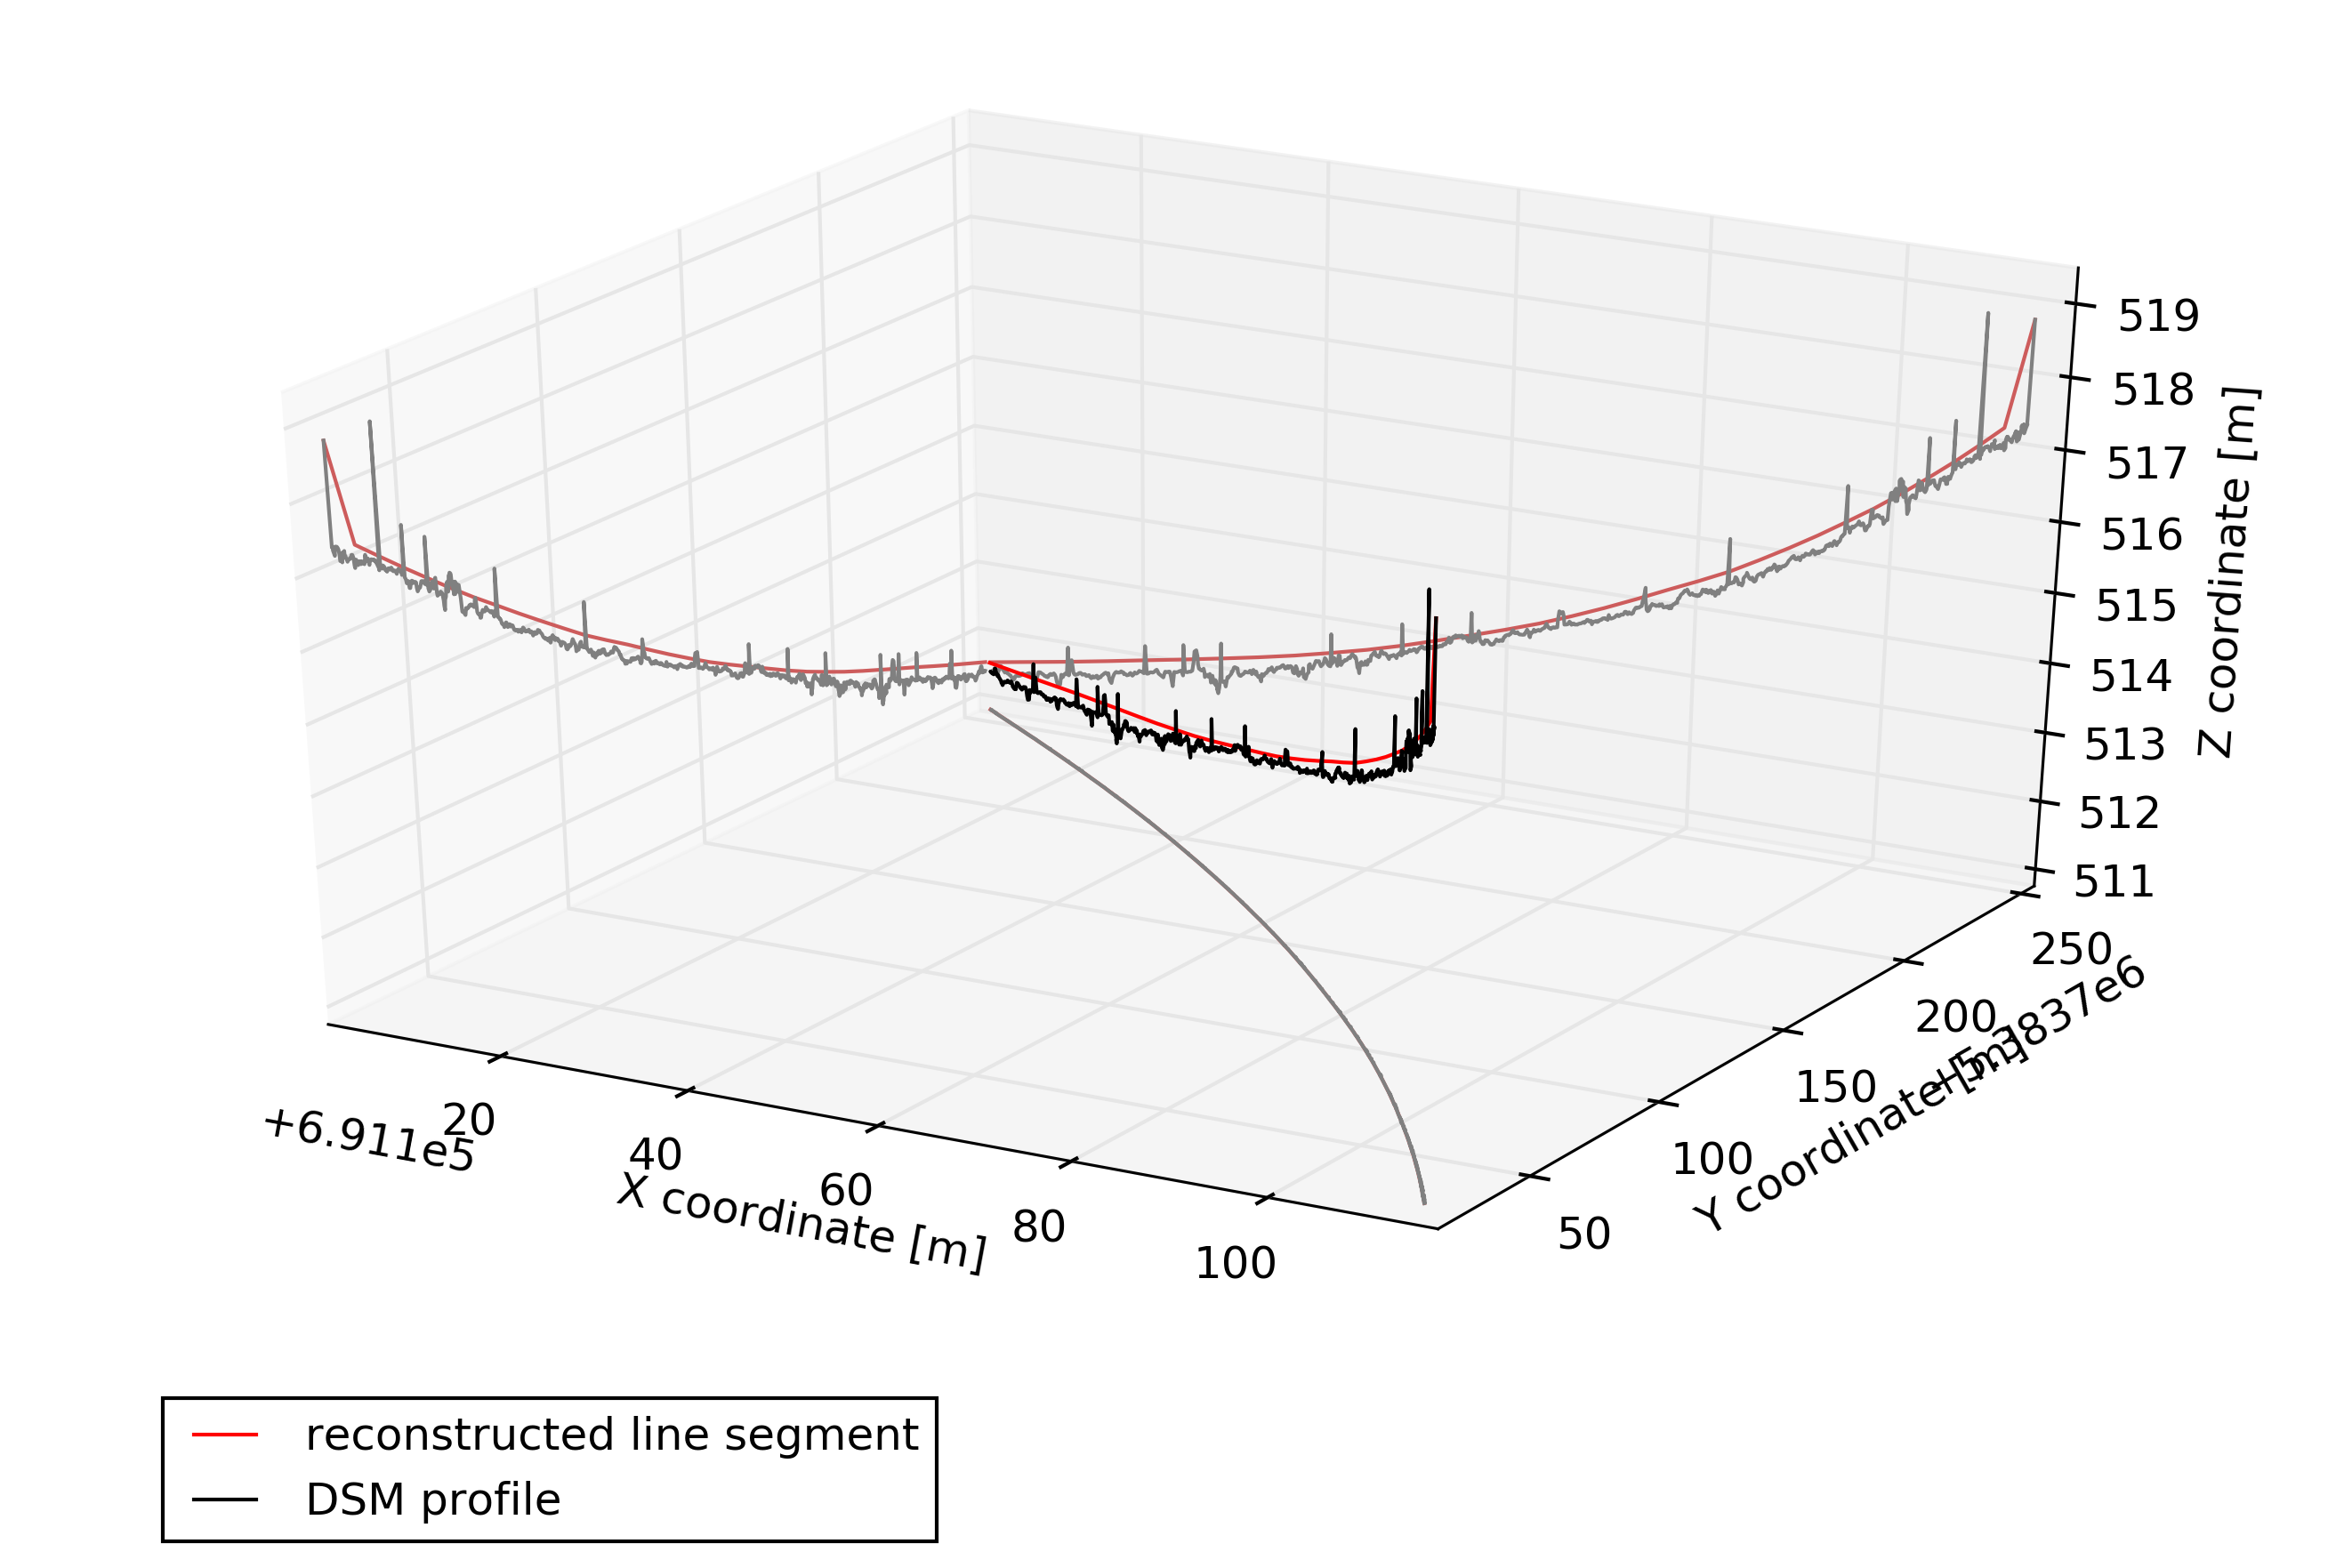
\includegraphics[width=\textwidth]{4_Test_3D.png} %%% 換,字重疊。
  \caption{\small The reconstructed line segments and the unrefined DSM profile in UTM coordinate system (in Zone 32N).}
  \label{fig:Test3D_1}
  \vspace{1cm}
  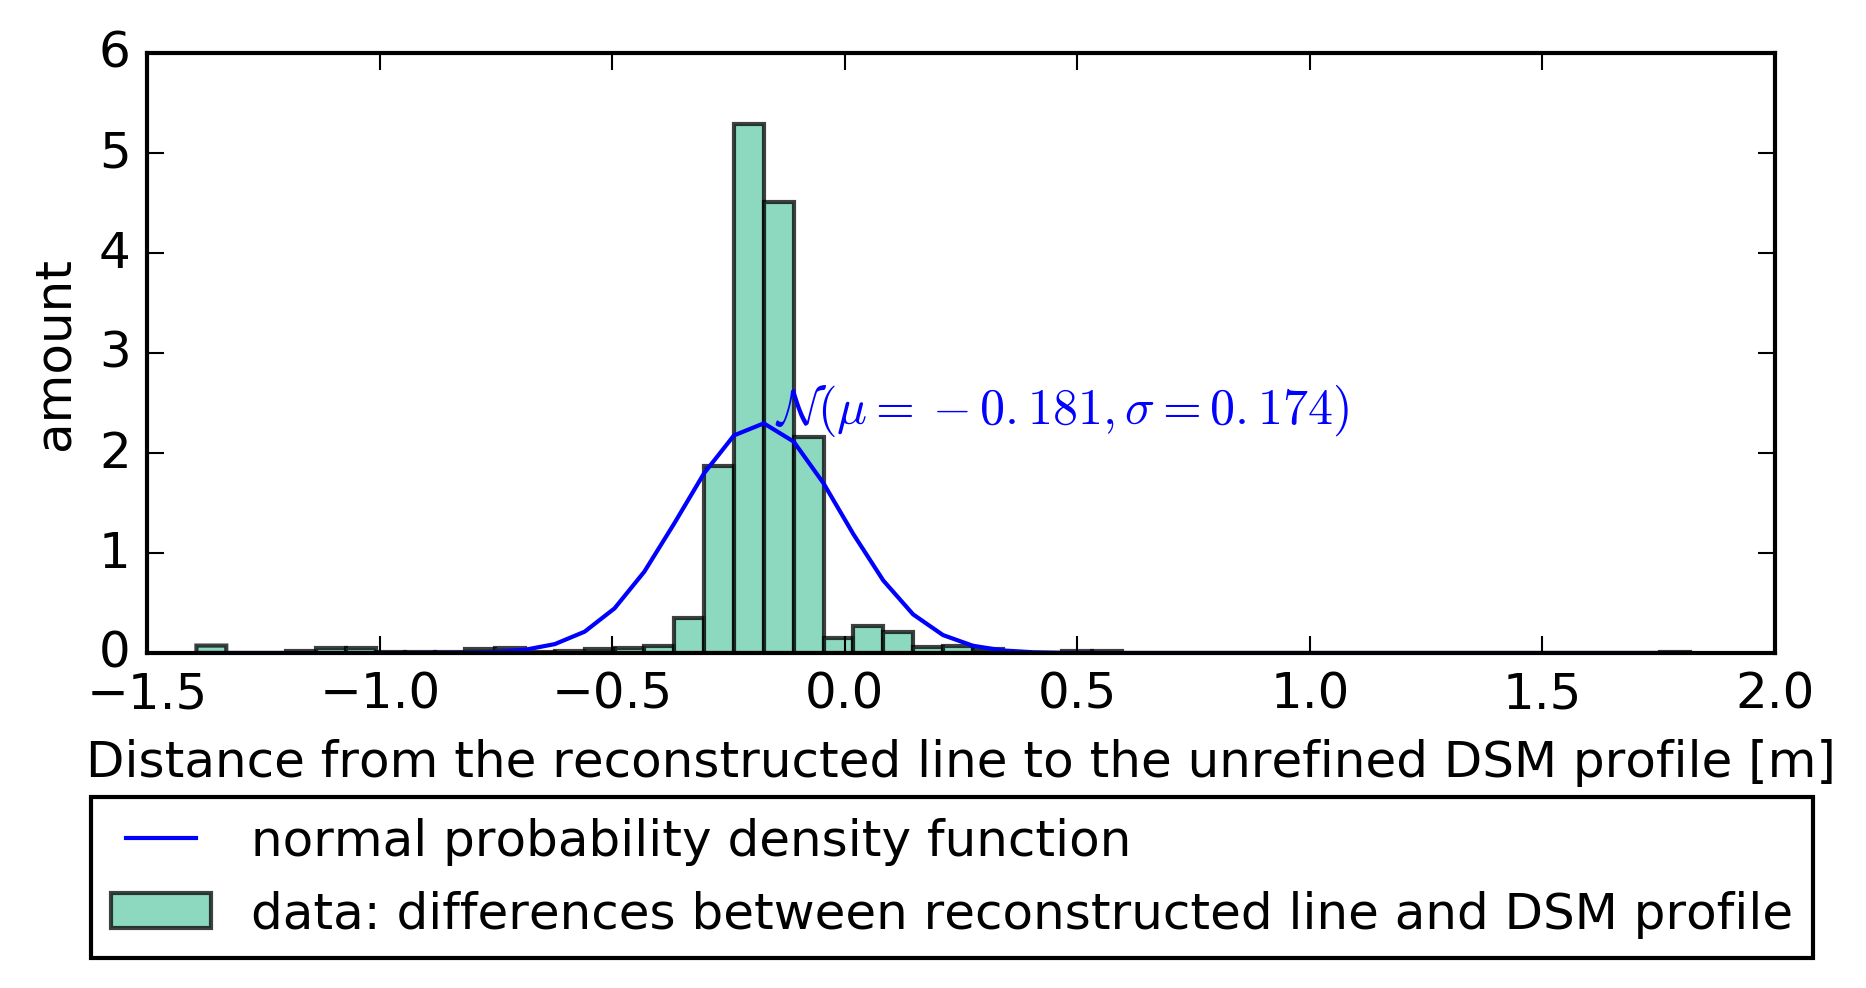
\includegraphics[width=\textwidth]{4_Test_hist.png} %%% 換,字太小、xlim。
  \caption{\small Histogram of the distances from the reconstructed line to the unrefined DSM profile.}
  \label{fig:TestHist_1}
\end{figure}

\clearpage

Images configuration plays an important roll in 3D reconstruction. %!!! discussion
\cref{fig:TestImgNum_1} shows: when more images cover a line segment, more measurements (extracted line segment) are provided, resulting higher redundancies in LS adjustment. (...???)

Since the estimated variance-covariance matrix of the estimated parameters $\hat{\Sigma}_{\hat{X}\hat{X}}$ depends on both the design matrix $A$ (i.e. the configuration) and the posterior standard deviation $\hat{\sigma}_0$ (i.e. the posterior measurements quality):
\begin{equation}
\hat{\Sigma}_{\hat{X}\hat{X}}=\hat{\sigma}_0^2(A^TA)^{-1}=
\begin{bmatrix}
\hat{\sigma}_{\hat{X}}^2 && \hat{\sigma}_{\hat{X}\hat{Y}} && \hat{\sigma}_{\hat{X}\hat{Z}} \\
\hat{\sigma}_{\hat{Y}\hat{X}} && \hat{\sigma}_{\hat{Y}}^2 && \hat{\sigma}_{\hat{Y}\hat{Z}} \\
\hat{\sigma}_{\hat{Z}\hat{X}} && \hat{\sigma}_{\hat{Z}\hat{Y}} && \hat{\sigma}_{\hat{Z}}^2
\end{bmatrix}
\end{equation}
we are not able to tell from the variances $\hat{\sigma}_{\hat{X}}$, $\hat{\sigma}_{\hat{Y}}$, $\hat{\sigma}_{\hat{Z}}$ whether the .

By setting a constant priori standard deviation value in all the LS adjustment processes (i.e. assuming the measurements are of same quality in each segment), the priori variance-covariance matrix of the estimated parameters $\Sigma_{\hat{X}\hat{X}}$ reflects the quality of the design matrix (i.e. the configuration strength) in each LS adjustment processes.
\begin{equation}
\Sigma_{\hat{X}\hat{X}}=\sigma_0^2(A^TA)^{-1}
\end{equation}

\cref{fig:TestdesignHV_1} shows:


\begin{figure}
  \centering
  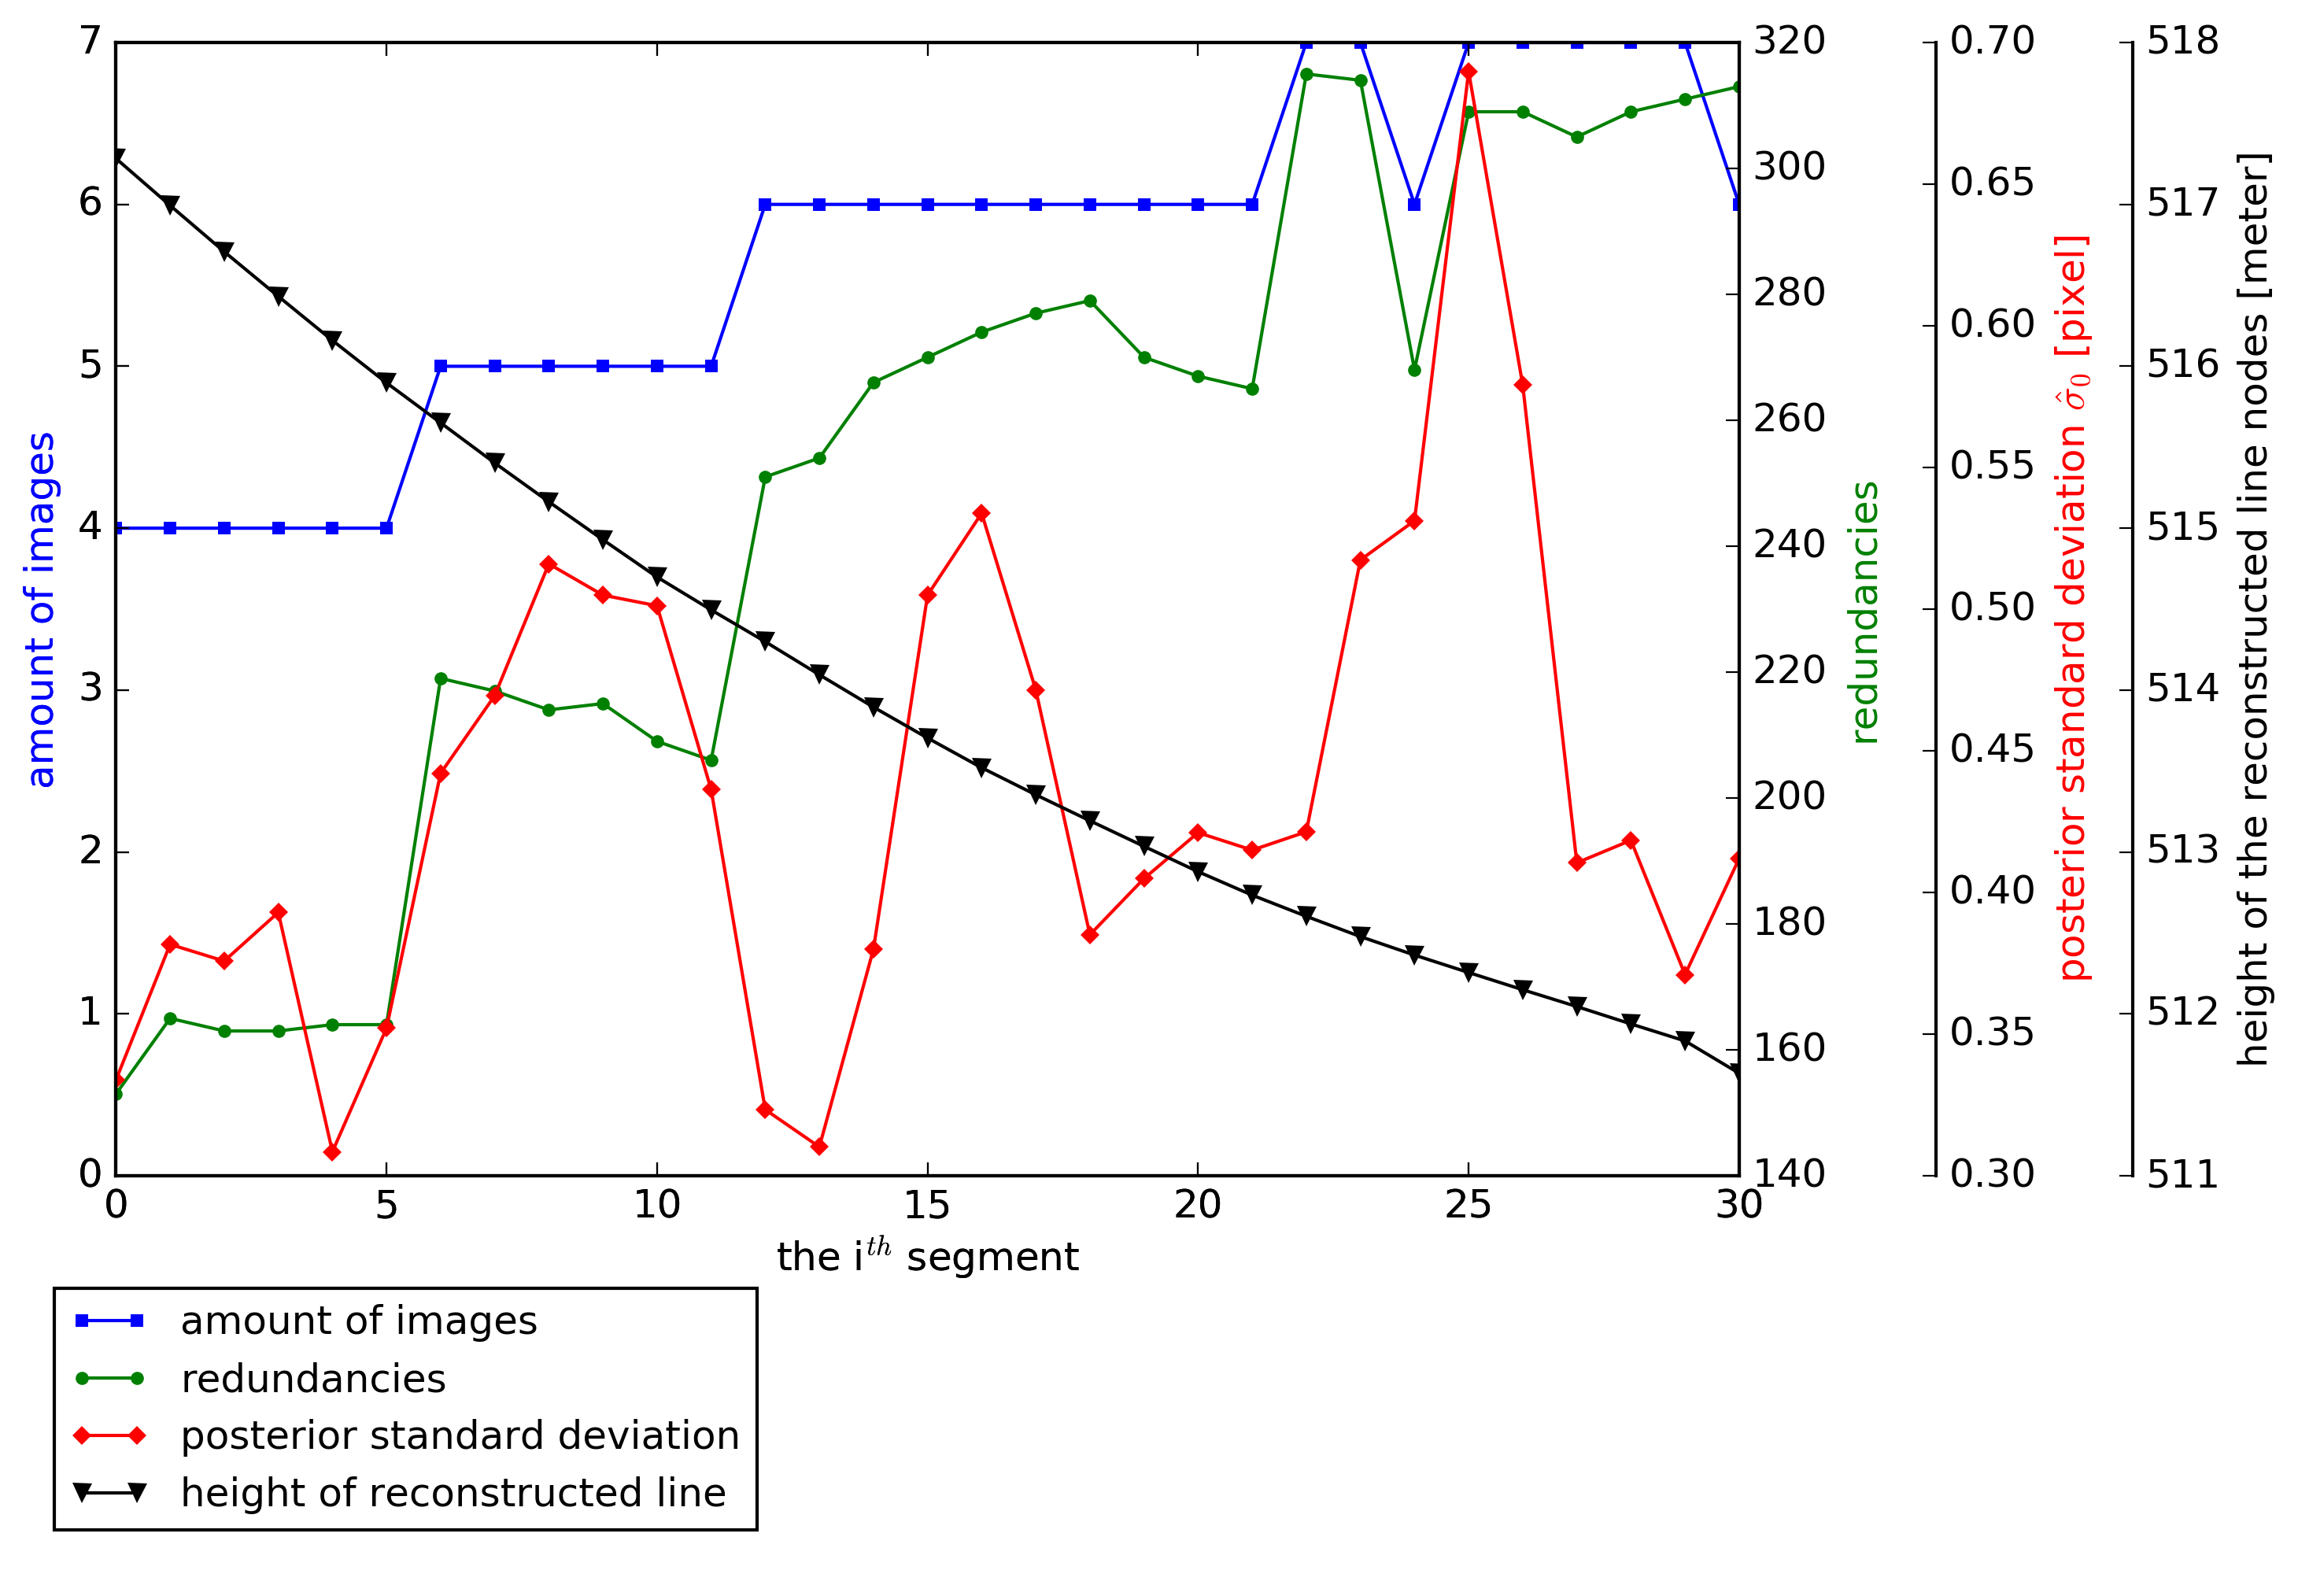
\includegraphics[width=0.95\textwidth]{4_Test_ImgNum.png} %%% 換,字重疊。
  \caption{\small The relationship between image amount, the resulting reconstructed line segments, and the redundancies and posterior standard deviation in LS adjustment.}
  \label{fig:TestImgNum_1}
  \vspace{1cm}
  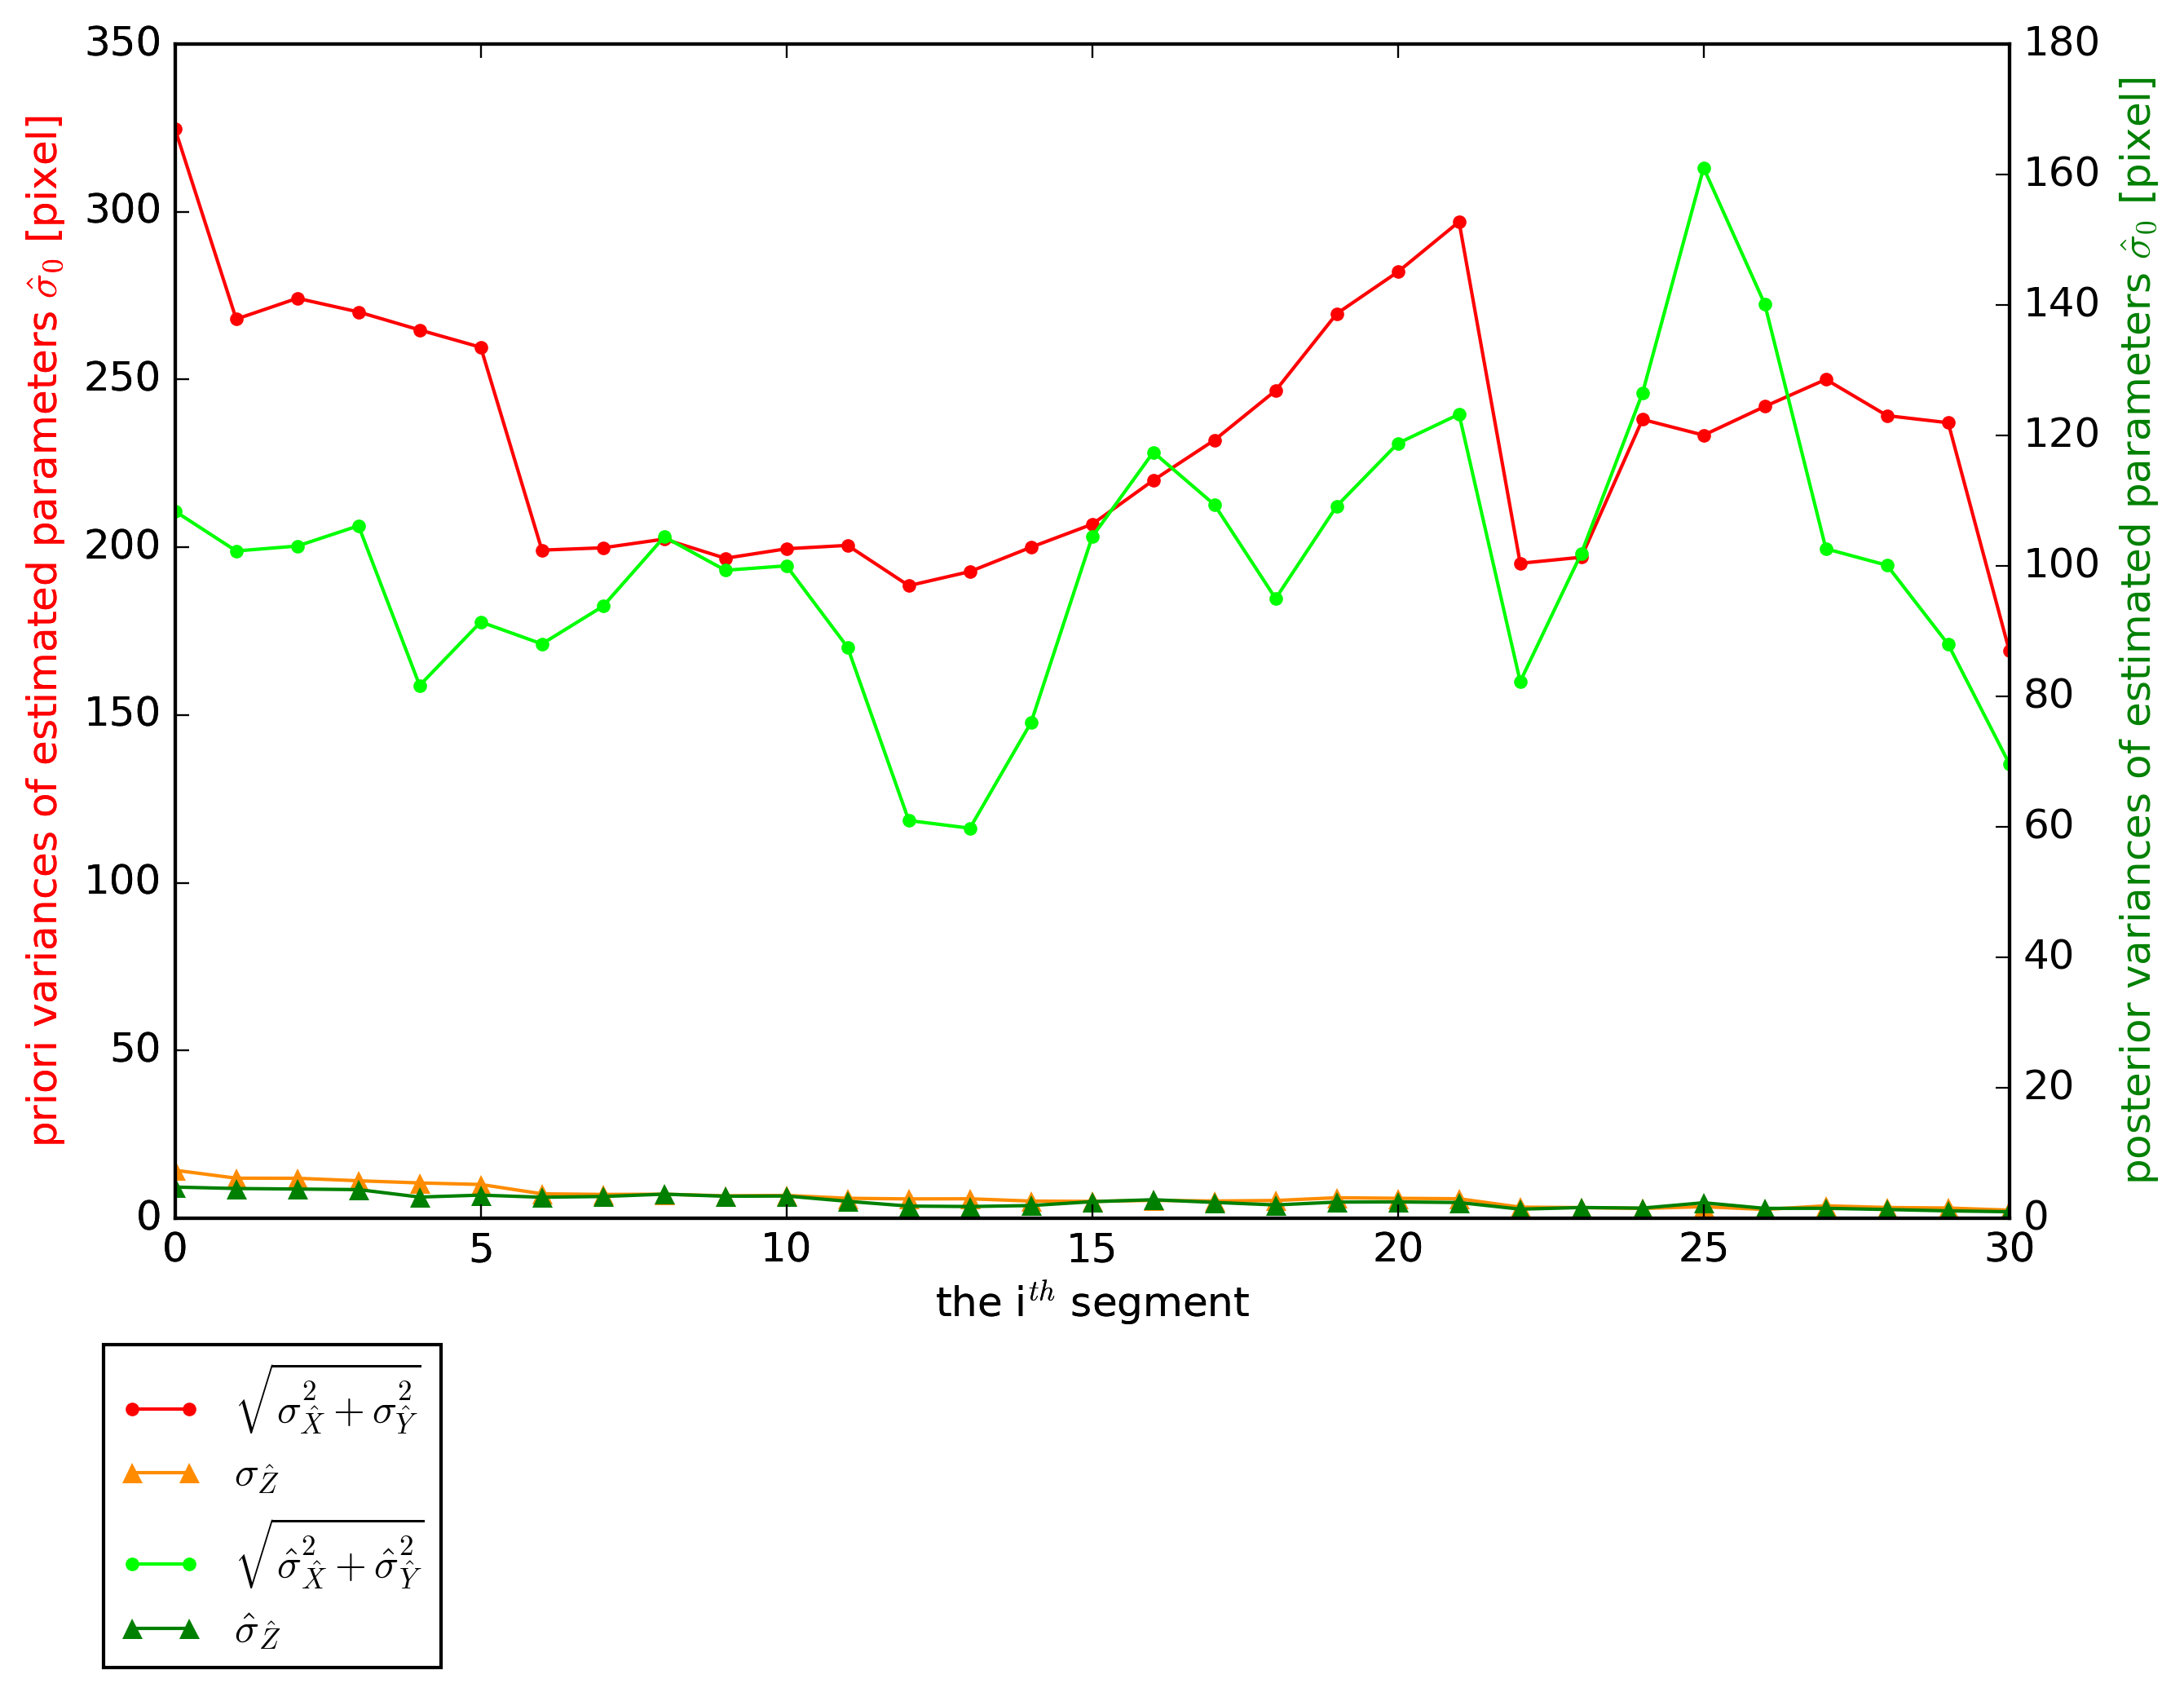
\includegraphics[width=0.8\textwidth]{4_Test_design_XY_Z.png} %%% 換,字太小、xlim。
  \caption{\small The variances of the estimated object coordinates, in horizontal and vertical directions, for both priori and posterior.}
  \label{fig:TestdesignHV_1}
\end{figure}


\clearpage

%\subsection{True Data Result: case2-5}
%\label{sec:trueresult-3}




%%%%%%%%%%%%%%%%%%%%%%%%%%%%%%%%%%%%%%%%%%%%%%%%%%%%%%%%
\section{Discussion: Influence of the Image Distribution and Amount}
\label{sec:discussion-ImageDistributionAmount}




%%%%%%%%%%%%%%%%%%%%%%%%%%%%%%%%%%%%%%%%%%%%%%%%%%%%%%%%
%3.1  Reference Data
%The primary reference dataset used in this paper is a 3D point cloud acquired by airborne laser scanning with a density of approximately 0.5 points per square meter.  The laser point cloud data is georeferenced in UTM Zone 31 North, ETRS89 and contains orthometric heights with respect to EGM 2008.  The orthometric  heights  were  converted  to  ellipsoidal  heights  by  simply dding the undulations from EGM 2008.  Only the first pulse returns is used in this study, as the DSM produced by image matching corresponds to the visible surface.  The LIDAR data for the errassa and Vacarisses test areas was acquired on 26th and 27th ovember 2007. The LaMola LIDAR data was acquired on 26th ovember 2007 and 4th May 2008

%%%%%%%%%%%%%%%%%%%%%%%%%%%%%%%%%%%%%%%%%%%%%%%%%%%%%%%%
4.3 Internal Factors

4.3.1 Correctness of

4.3.2 Verification of

4.3.3 Precision of


%%%%%%%%%%%%%%%%%%%%%%%%%%%%%%%%%%%%%%%%%%%%%%%%%%%%%%%%
4.4 External Factors

4.4.1 Influence of 

%noch etwas Fülltext
%\blinddocument

% !TeX spellcheck = de_DE

\chapter{Conclusion and Future Work}
\label{chap:conclusion}

This thesis proposed a framework for automatic 3D lane marking reconstruction using multi-view aerial imagery. Standard line detection algorithms are applied to extract lane markings on the aerial images. By exploiting the use of linear regression in image space and with the combination of collinearity condition, lane markings are reconstructed based on their detected positions in images and the viewing geometry. Without the utilization of the neighboring textures, the approach requires initial approximate 3D lines and is highly dependent on quality of pre-known image orientations. Nevertheless, it is robust to partial occlusions of the targeted lines on images and is applicable to the (quasi-)infinite line features as well as in cases of lowly textured neighboring and it improves the DSM at lowly textured road surfaces. 


From simulated experiments in \cref{sec:simulation}, some conclusions are given:
\begin{itemize}
	\item Given approximations with 2 meters bias in Z-direction and sub-pixel random noises in the image coordinates of the detected/measured 2D lines, the proposed approach correctly refined the 3D positions of line segments.
	
	\item With the same line orientations in 3D space, the configuration strength increases with the increase of amount of covering images from different views.
	
	\item The reconstructed line segments have higher priori precision in horizontal direction than in vertical direction.
\end{itemize}


From experimental results of true data in \cref{sec:simulation}, some conclusions are given:
\begin{itemize}
	\item The DSM profile, i.e. the initial 3D line approximation, is significantly and systematically dozens of centimeters far away from the reconstructed line segments. This indicates the necessity of reconstrucion based on detected 2D lines in image space and the viewing geometry, instead of simply reducing DSM noise by applying mean filter or such.
	
	\item The LS-estimated precision of the measurements, involving the lane marking extraction quality as well as the quality of image orientation parameters, is better than 1 pixel.

	\item The configuration defect %which is mentioned in \cref{subsec:LSadj} 
	barely happens: 1.when the linear regression functional model between image coordinates $x$ and $y$ are properly set up ---according to the characteristics of the detected lane-lines in image space. 2.when the flight configuration guarantees stereo views whose base-lines are perpendicular to lane-lines orientations in 3D.
	
	\item The theoretical precision of the reconstructed line-nodes is within 2.5 cm in vertical direction and within 5 mm in horizontal direction.
%	\item  %The configuration defect in object space %which is mentioned in \cref{subsec:LSadj} 
%	%may happen in some of the stereo views in the same strip with the adopted flight configuration in this work.% of flying along the motorways, the detected lane lines lie mainly in flight direction on images.
%	With the adopted flight configuration in this work, the stereo pairs in the same strip, where the lane markings lie nearly on the epipolar plane, barely contribute on increasing the configuration strength for lane marking reconstruction. 
%	%This indirectly indicates that, under this kind of image configuration, increasing forward overlapping rate does not really increase the configuration strength for 3D lane markings reconstruction. 
	
\end{itemize}


%using precisely detected lines with sub-pixel precision as well the bundle adjusted image orientations, the lane markings can be reconstructed with ???centimeter accuracy??? using well configured aerial images.

%With the extracted line in the form of sets of points with sub-pixel accuracy and EOIO accuracy???, linear regression can be applied on reconstructing the 3D line segment position.

%image distortion vs straight line approximation

Some general conclusions are:
\begin{itemize}
	\item Image configuration plays an important roll in 3D reconstruction. In the case of this work, being covered by more views whose base-lines are as perpendicular as possible to lane-marking directions, would improve the reconstruction result.
	
	\item Lane markings can be exploited to provide information on refining SGM-generated DSM.% Reconstruction based on imaging geometry is necessary.

	\item The proposed reconstruction workflow relies on initial approximation with enough accuracy, i.e. a global terrain model like SRTM would not be sufficient as starting height, as the error could be several meters in particular at roads.
\end{itemize}





\section*{Future Work}
\label{chap:futurework}

%Future improvements could be achieved by:

%having crab angles of $\approx45\degree$ in flight.
%Theoretically this kind of configuration defect may be solved.

%increasing the oblique angle
The proposed approach addresses 3D line features reconstruction problems without resorting to their appearances in images. Similar cases are railways. Appling this framwork to such cases may be done in the future. Additionally, it worths trying the framework with images taken from drones instead of from helicopters.


%
%
%\renewcommand{\appendixtocname}{Anhang}
%\renewcommand{\appendixname}{Anhang}
%\renewcommand{\appendixpagename}{Anhang}
%\appendix
%% !TeX spellcheck = de_DE
%Die Angabe des schlauen Spruchs auf diesem Wege funtioniert nur,
%wenn keine Änderung des Kapitels mittels den in preambel/chapterheads.tex
%vorgeschlagenen Möglichkeiten durchgeführt wurde.
\setchapterpreamble[u]{%
\dictum[Albert Einstein]{Probleme kann man niemals mit derselben Denkweise lösen, durch die sie entstanden sind.}
}
\chapter{LaTeX-Tipps}
\label{chap:latextipps}

Pro Satz eine neue Zeile.
Das ist wichtig, um sauber versionieren zu können.
In LaTeX werden Absätze durch eine Leerzeile getrennt.

Folglich werden neue Abstäze insbesondere \emph{nicht} durch Doppelbackslashes erzeugt.
Der letzte Satz kam in einem neuen Absatz.

\section{File-Encoding und Unterstützung von Umlauten}
\label{sec:firstsectioninlatexhints}
Die Vorlage wurde 2010 auf UTF-8 umgestellt.
Alle neueren Editoren sollten damit keine Schwierigkeiten haben.

\section{Zitate}
Referenzen werden mittels \texttt{\textbackslash cite[key]} gesetzt.
Beispiel: \cite{WSPA} oder mit Autorenangabe: \citet{WSPA}.

Der folgende Satz demonstriert \begin{inparaenum}[1.]
\item die Großschreibung von Autorennamen am Satzanfang,
\item die richtige Zitation unter Verwendung von Autorennamen und der Referenz,
\item dass die Autorennamen ein Hyperlink auf das Literaturverzeichnis sind sowie
\item dass in dem Literaturverzeichnis der Namenspräfix \enquote{van der} von \enquote{Wil M.\,P.\ van der Aalst} steht.
\end{inparaenum}
\Citet{RVvdA2016} präsentieren eine Studie über die Effektivität von Workflow-Management-Systemen.

Der folgende Satz demonstriert, dass man mittels \texttt{label} in einem Bibliopgrahie"=Eintrag den Textteil des generierten Labels überschreiben kann, aber das Jahr und die Eindeutigkeit noch von biber generiert wird.
Die Apache ODE Engine \cite{ApacheODE} ist eine Workflow-Maschine, die BPEL-Prozesse zuverlässig ausführt.

Wörter am besten mittels \texttt{\textbackslash enquote\{...\}} \enquote{einschließen}, dann werden die richtigen Anführungszeichen verwendet.

Beim Erstellen der Bibtex-Datei wird empfohlen darauf zu achten, dass die DOI aufgeführt wird.

\section{Mathematische Formeln}
\label{sec:mf}
Mathematische Formeln kann man $so$ setzen. \texttt{symbols-a4.pdf} (zu finden auf \url{http://www.ctan.org/tex-archive/info/symbols/comprehensive/symbols-a4.pdf}) enthält eine Liste der unter LaTeX direkt verfügbaren Symbole.
Z.\,B.\ $\mathbb{N}$ für die Menge der natürlichen Zahlen.
Für eine vollständige Dokumentation für mathematischen Formelsatz sollte die Dokumentation zu \texttt{amsmath}, \url{ftp://ftp.ams.org/pub/tex/doc/amsmath/} gelesen werden.

Folgende Gleichung erhält keine Nummer, da \texttt{\textbackslash equation*} verwendet wurde.
\begin{equation*}
x = y
\end{equation*}

Die Gleichung~\ref{eq:test} erhält eine Nummer:
\begin{equation}
\label{eq:test}
x = y
\end{equation}

Eine ausführliche Anleitung zum Mathematikmodus von LaTeX findet sich in \url{http://www.ctan.org/tex-archive/help/Catalogue/entries/voss-mathmode.html}.

\section{Quellcode}
\Cref{lst:ListingANDlstlisting} zeigt, wie man Programmlistings einbindet.
Mittels \texttt{\textbackslash lstinputlisting} kann man den Inhalt direkt aus Dateien lesen.

%Listing-Umgebung wurde durch \newfloat{Listing} definiert
\begin{Listing}
\begin{lstlisting}
<listing name="second sample">
  <content>not interesting</content>
</listing>
\end{lstlisting}
\caption{lstlisting in einer Listings-Umgebung, damit das Listing durch Balken abgetrennt ist}
\label{lst:ListingANDlstlisting}
\end{Listing}

Quellcode im \lstinline|<listing />| ist auch möglich.

\section{Abbildungen}

Die \cref{fig:chor1} und \ref{fig:chor2} sind für das Verständnis dieses Dokuments wichtig.
Im Anhang zeigt \vref{fig:AnhangsChor} erneut die komplette Choreographie.

%Die Parameter in eckigen Klammern sind optionale Parameter - z.B. [htb!]
%htb! bedeutet: "Liebes LaTeX, bitte platziere diese Abbildung zuerst hier ("_h_ere"). Falls das nicht funktioniert, dann bitte oben auf der Seite ("_t_op"). Und falls das nicht geht, bitte unten auf der Seite ("_b_ottom"). Und bitte, bitte bevorzuge hier und oben, auch wenn's net so optimal aussieht ("!")
%Diese sollten nach Möglichkeit NICHT verwendet werden. LaTeX's Algorithmus für das Platzieren der Gleitumgebung ist schon sehr gut!
\begin{figure}
  \centering
  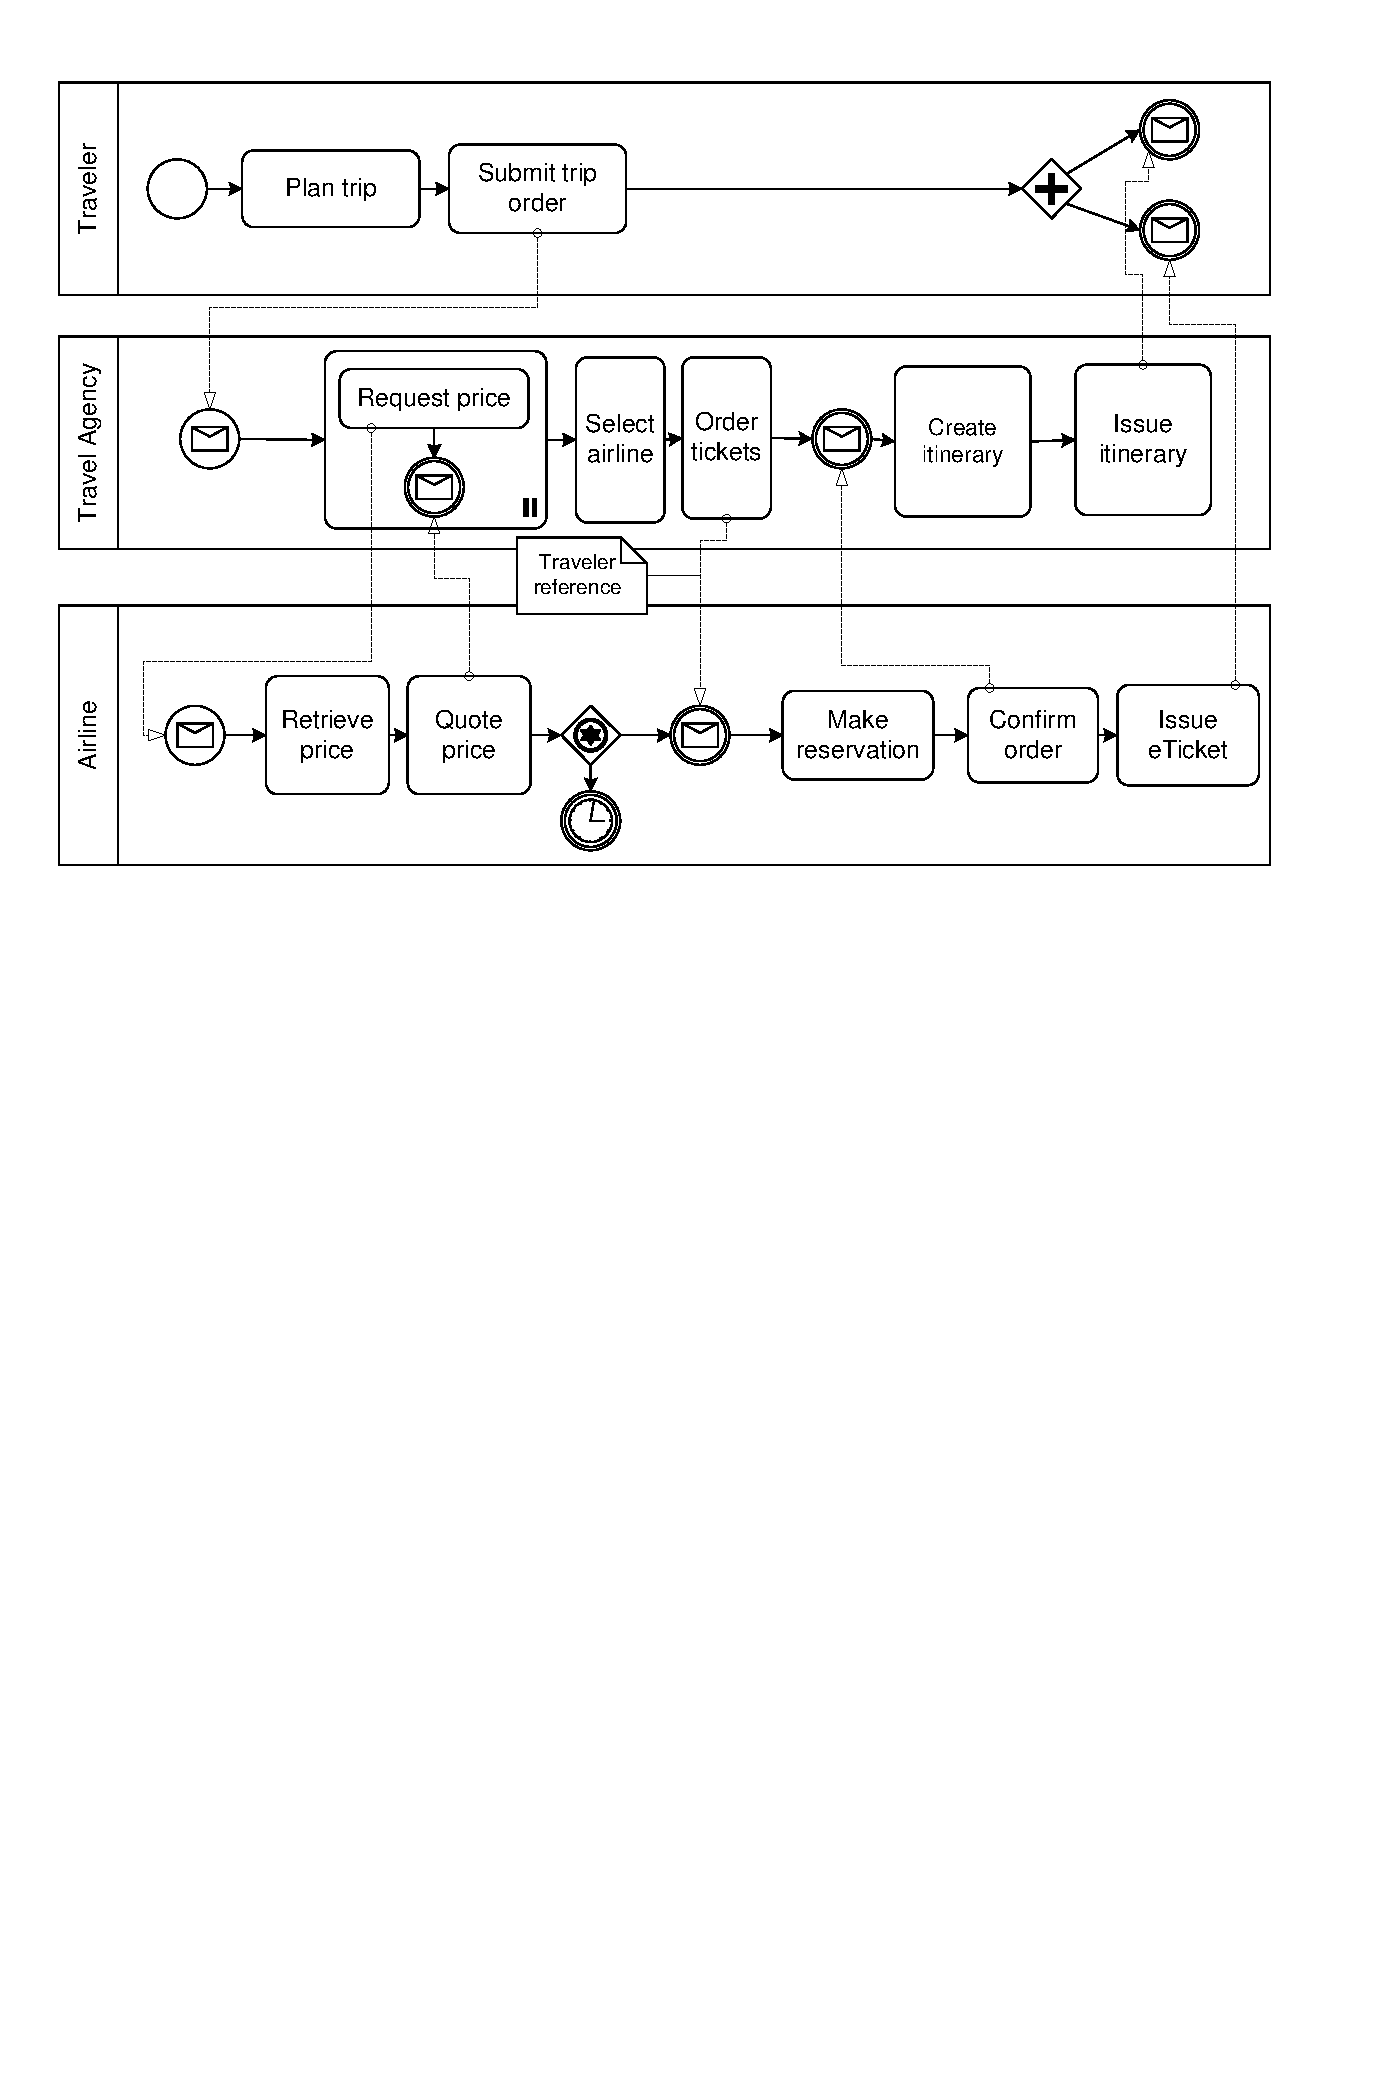
\includegraphics[width=\textwidth]{choreography.pdf}
  \caption{Beispiel-Choreographie}
  \label{fig:chor1}
\end{figure}

\begin{figure}
  \centering
  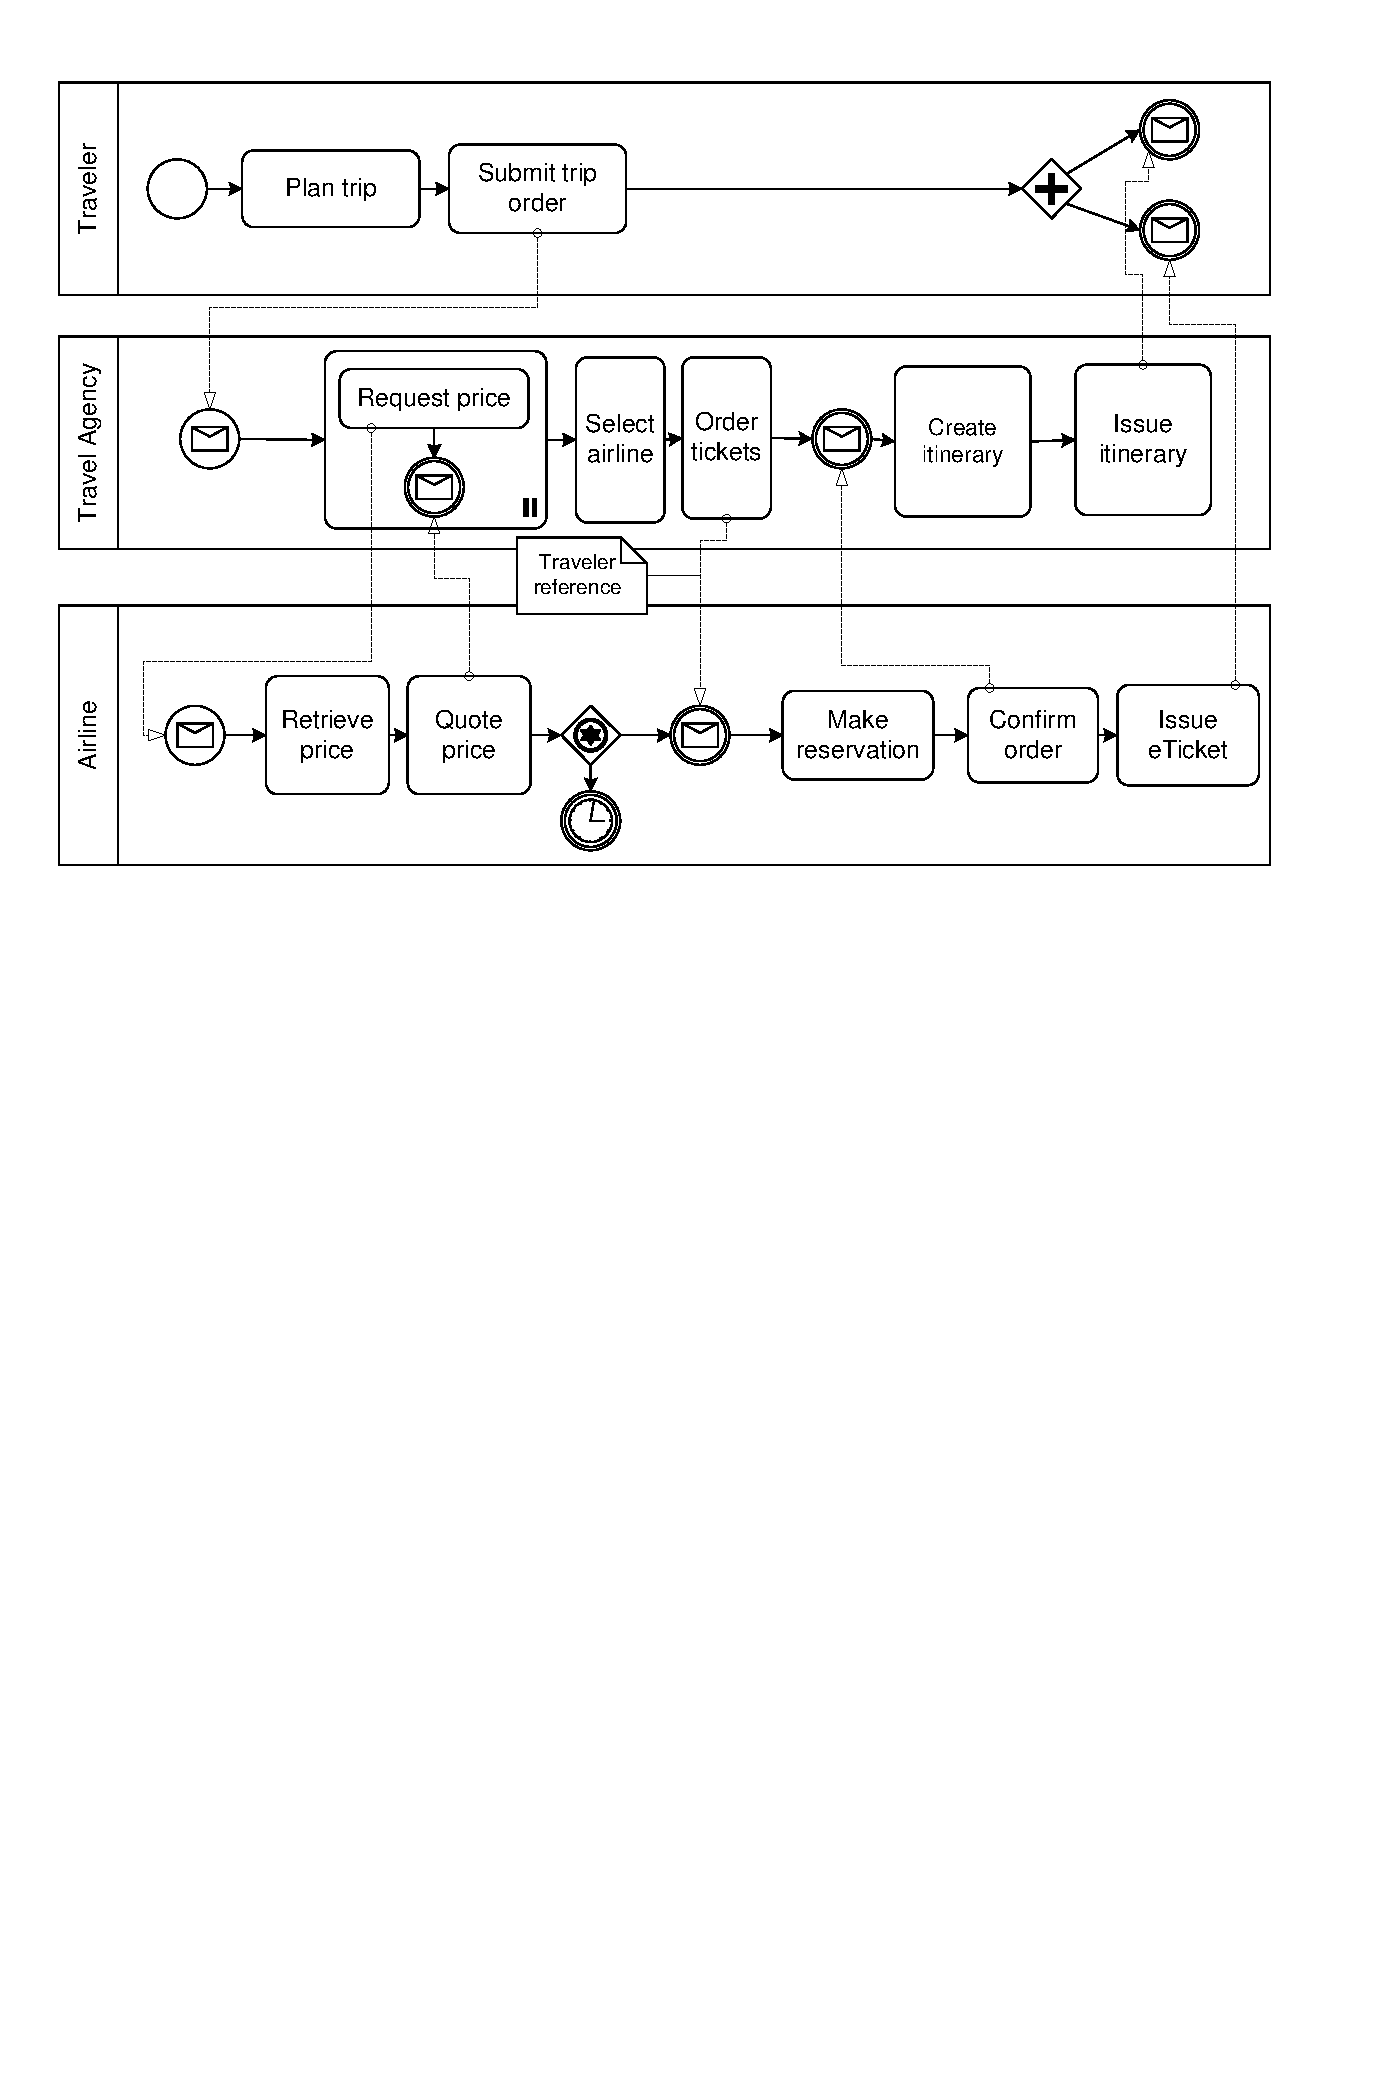
\includegraphics[width=.8\textwidth]{choreography.pdf}
  \caption[Beispiel-Choreographie]{Die Beispiel-Choreographie. Nun etwas kleiner, damit \texttt{\textbackslash textwidth} demonstriert wird. Und auch die Verwendung von alternativen Bildunterschriften für das Verzeichnis der Abbildungen. Letzteres ist allerdings nur Bedingt zu empfehlen, denn wer liest schon so viel Text unter einem Bild? Oder ist es einfach nur Stilsache?}
  \label{fig:chor2}
\end{figure}


\begin{figure}
  \centering
    \subfloat[]{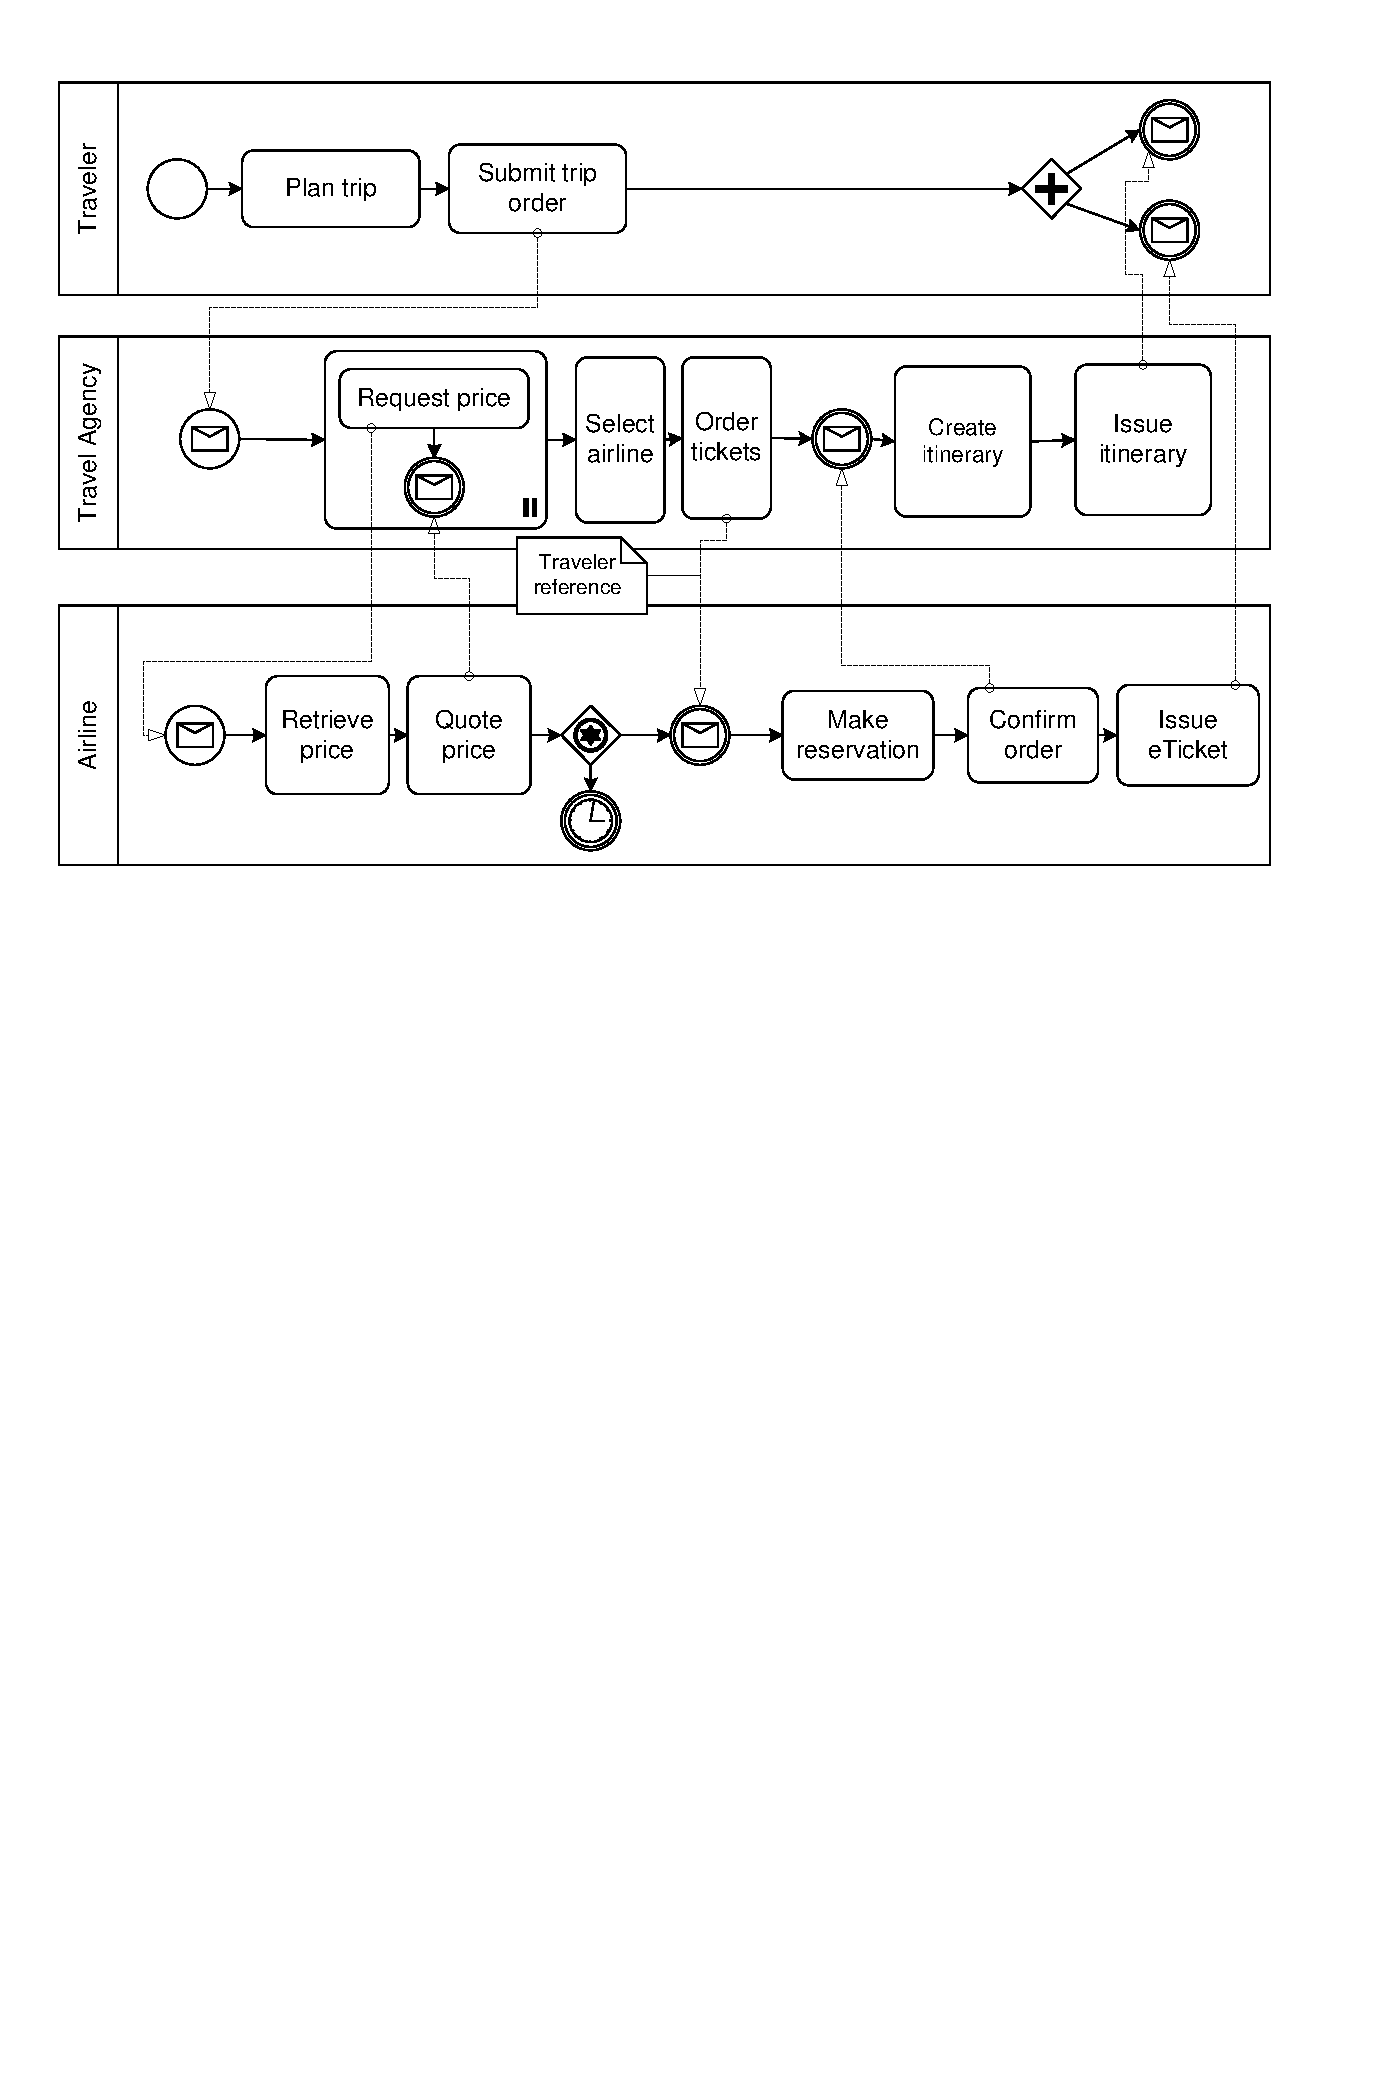
\includegraphics[width=0.3\textwidth]{choreography.pdf} \label{fig:subfigA}}
    \subfloat[]{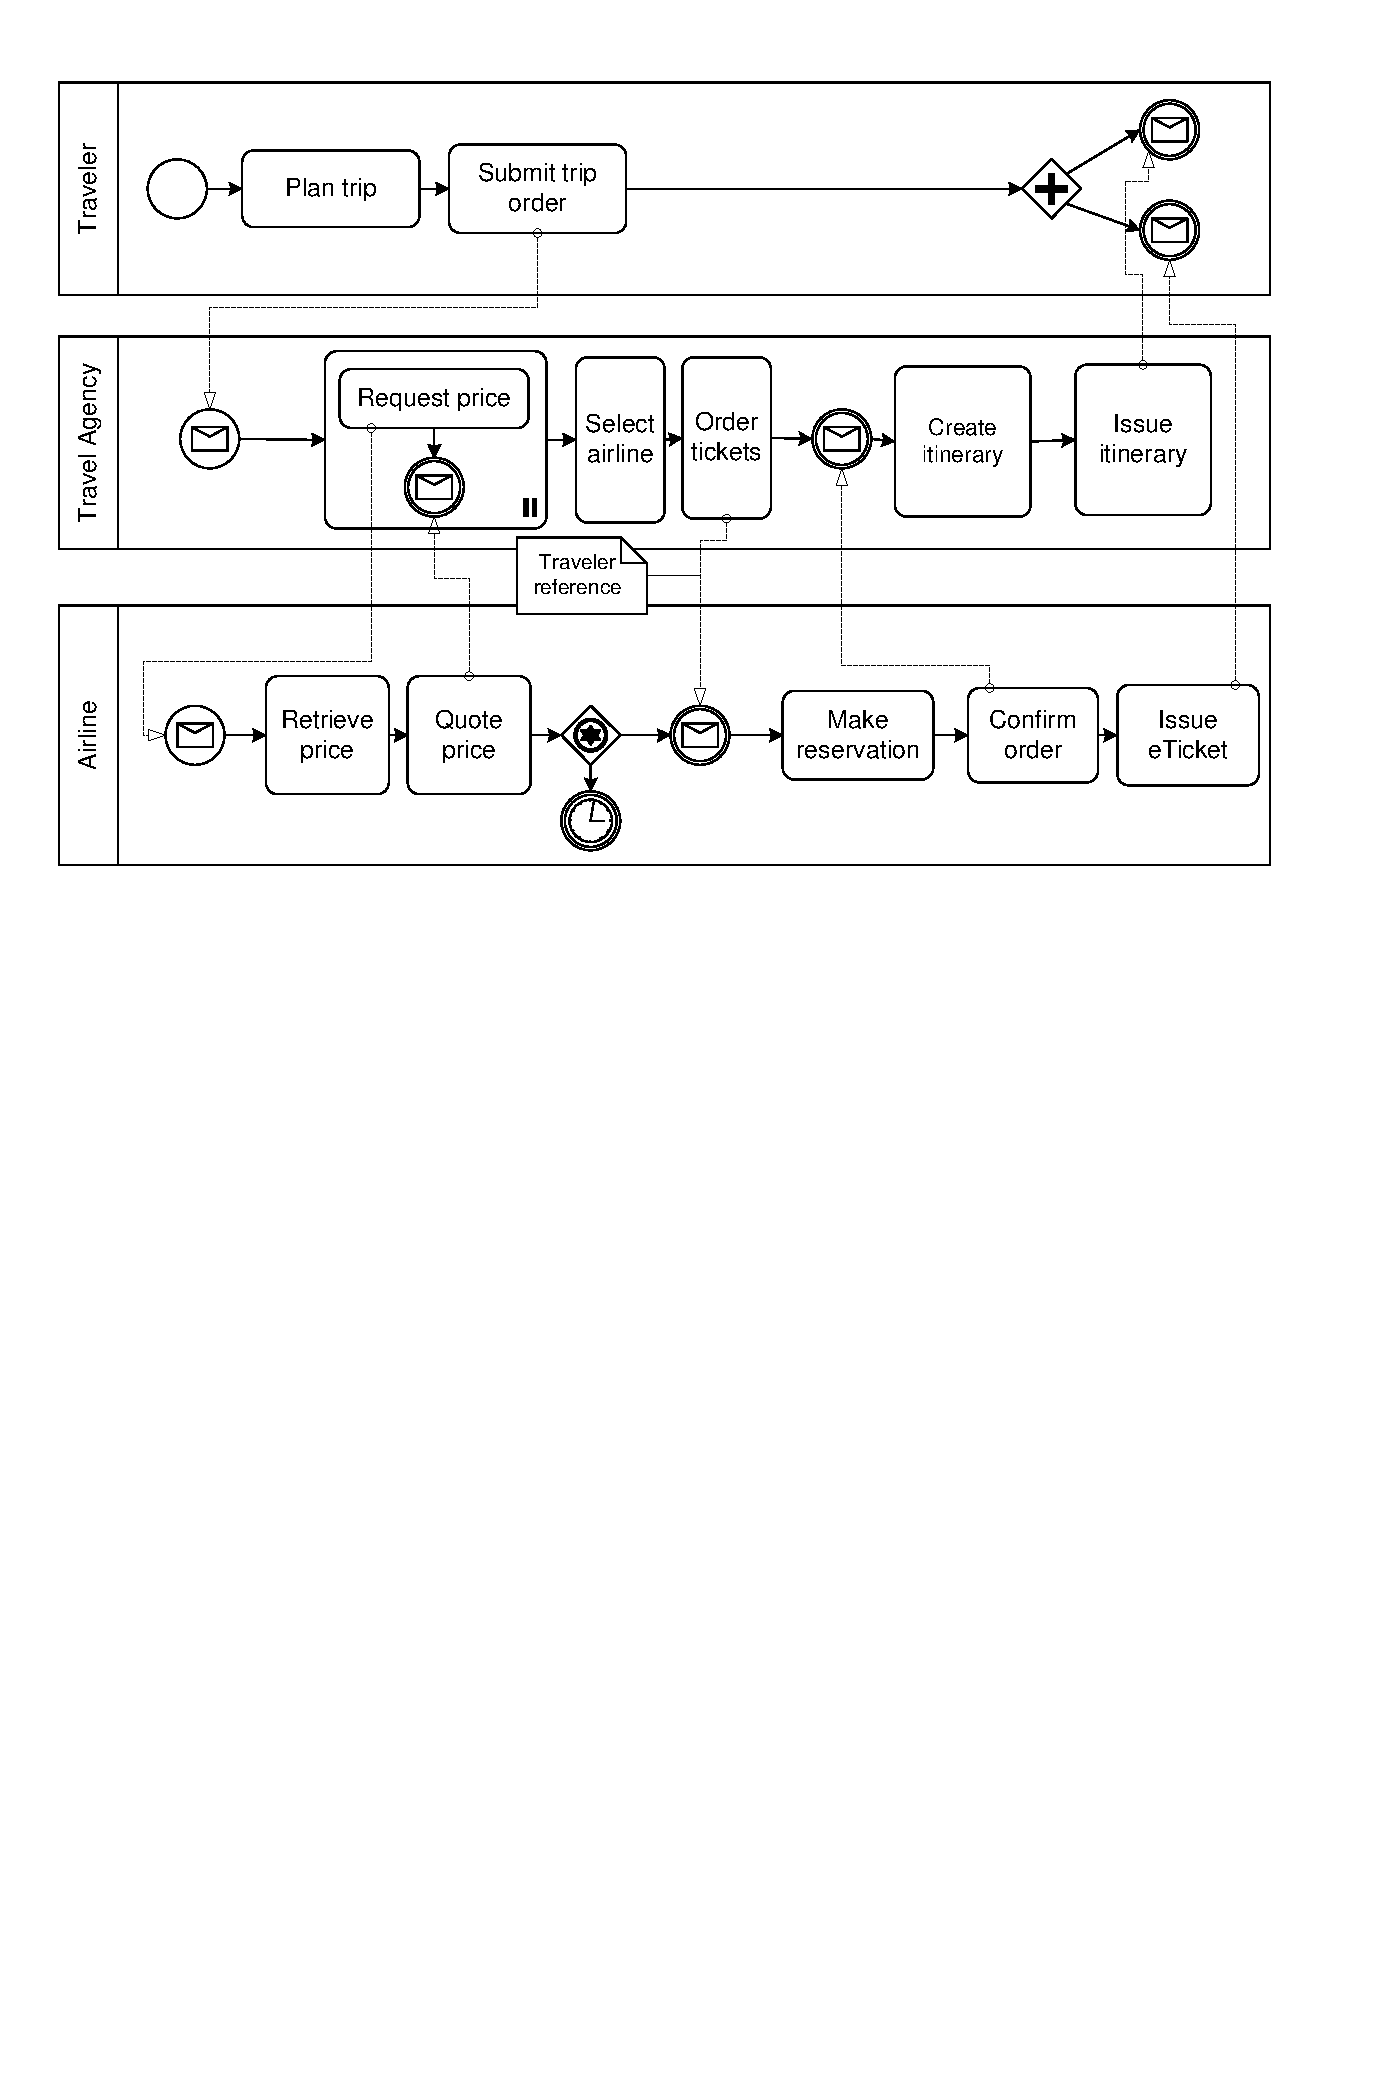
\includegraphics[width=0.3\textwidth]{choreography.pdf} \label{fig:subfigB}}
		\subfloat[Subcaption if needed]{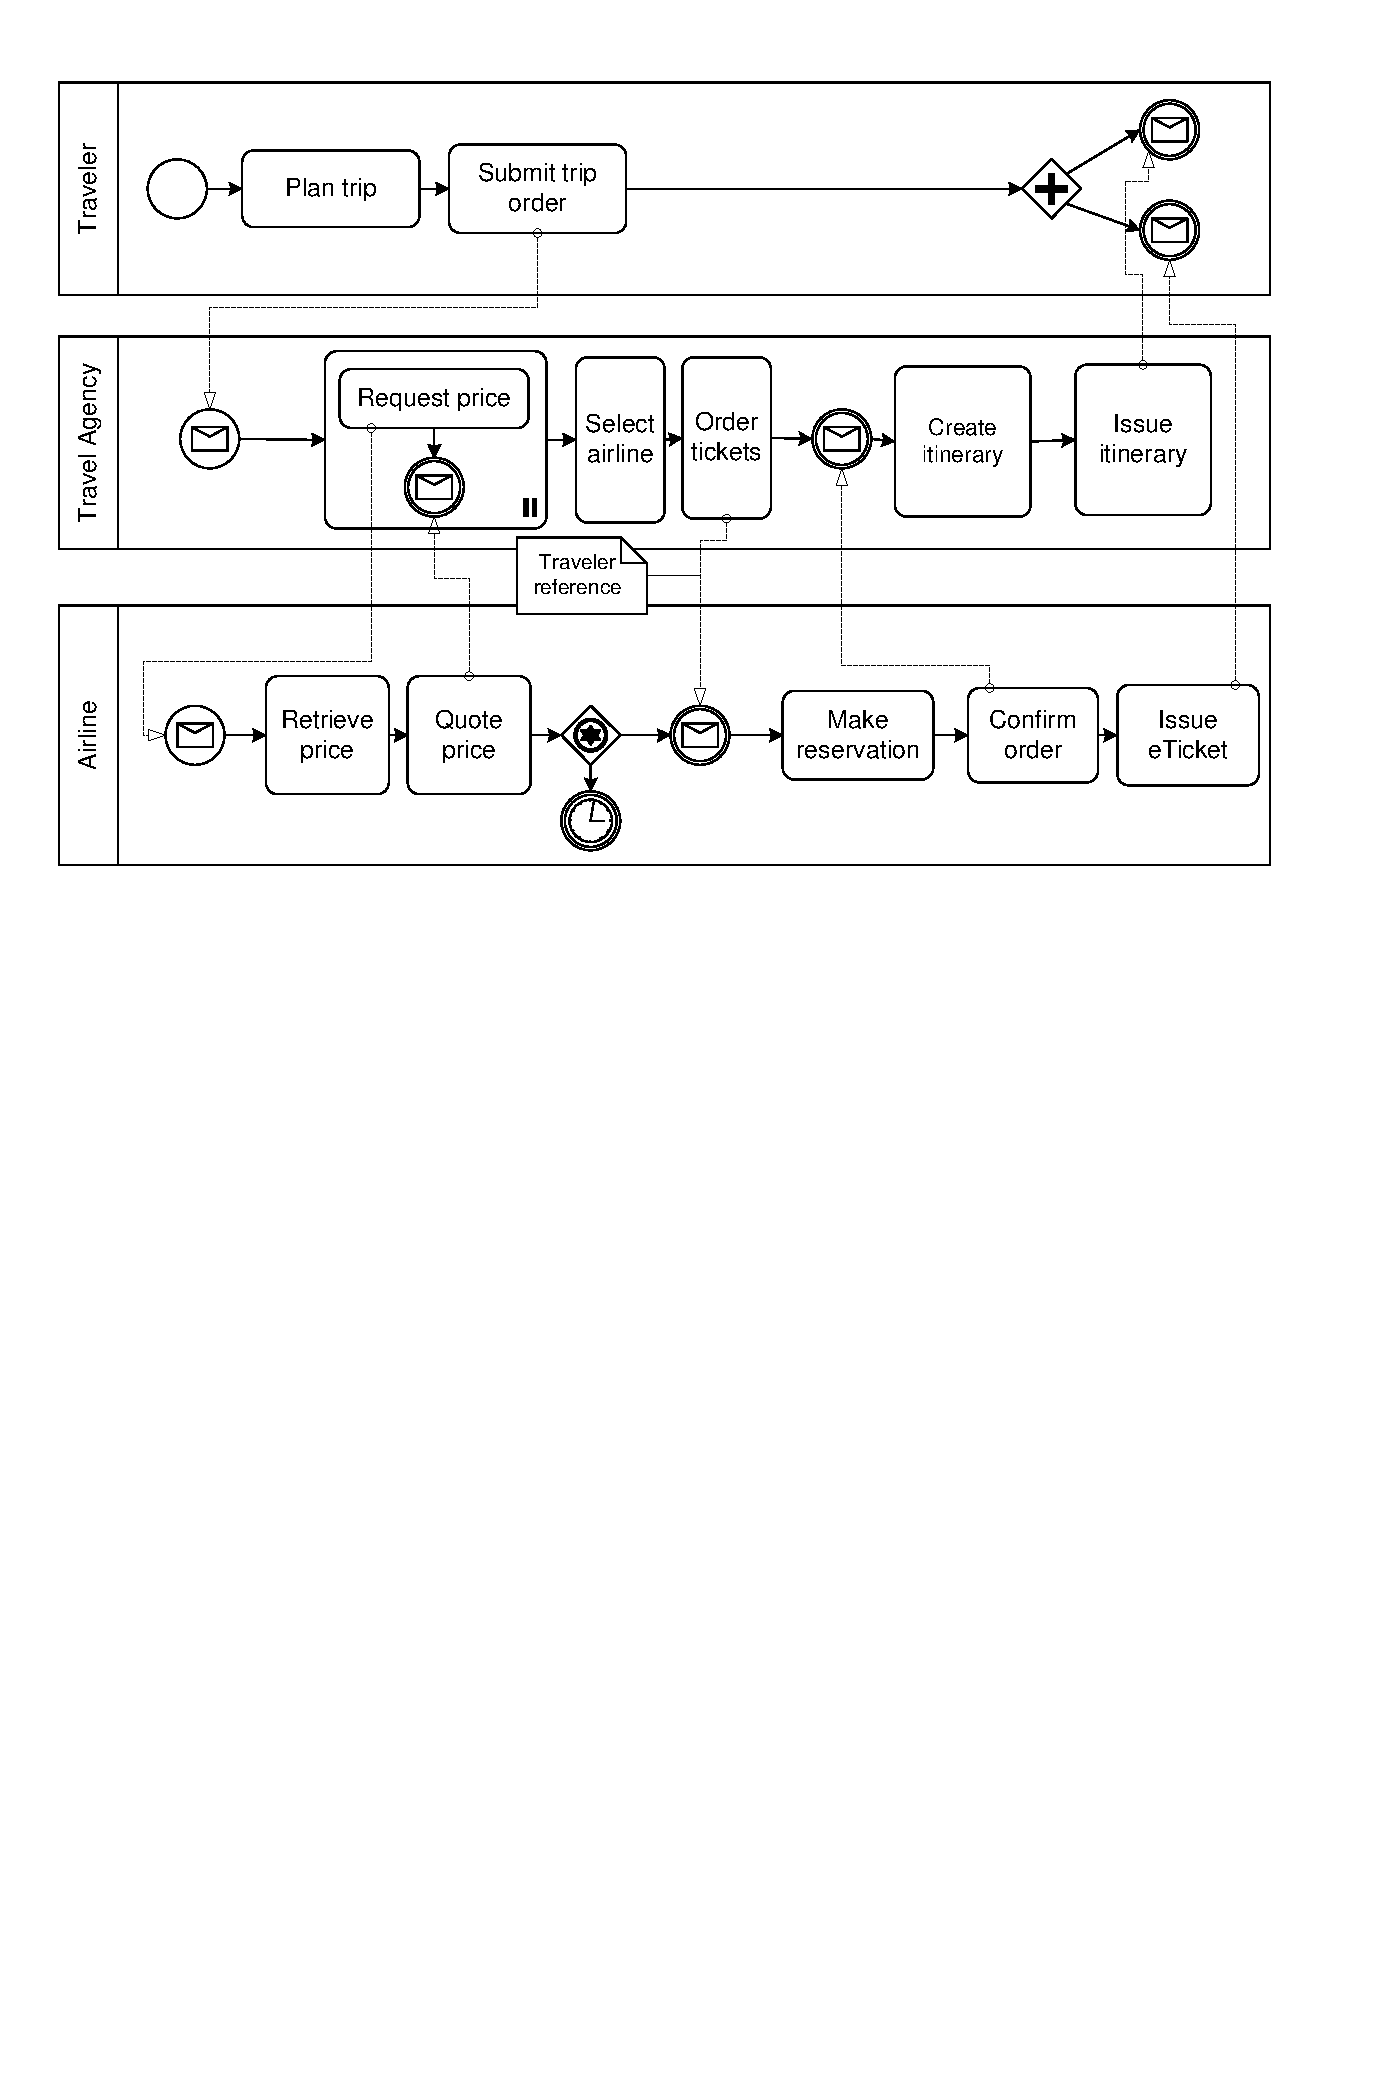
\includegraphics[width=0.3\textwidth]{choreography.pdf} \label{fig:subfigC}}
	\caption{Beispiel um 3 Abbildung nebeneinader zu stellen nur jedes einzeln referenzieren zu können. Abbildung~\ref{fig:subfigB}
 ist die mittlere Abbildung.}
\label{fig:subfig_example}
\end{figure}

Es ist möglich, SVGs direkt beim Kompilieren in PDF umzuwandeln.
Dies ist im Quellcode zu latex-tipps.tex beschrieben, allerdings auskommentiert.

\iffalse % <-- Das hier wegnehmen, falls inkscape im Pfad ist
Das SVG in \cref{fig:directSVG} ist direkt eingebunden, während der Text im SVG in \cref{fig:latexSVG} mittels pdflatex gesetzt ist.
Falls man die Graphiken sehen möchte, muss inkscape im PATH sein und im Tex-Quelltext \texttt{\textbackslash{}iffalse} und \texttt{\textbackslash{}iftrue} auskommentiert sein.

\begin{figure}
\centering

\includegraphics{svgexample.svg}
\caption{SVG direkt eingebunden}
\label{fig:directSVG}
\end{figure}

\begin{figure}
\centering
\def\svgwidth{.4\textwidth}
\includesvg{svgexample}
\caption{Text im SVG mittels \LaTeX{} gesetzt}
\label{fig:latexSVG}
\end{figure}
\fi % <-- Das hier wegnehmen, falls inkscape im Pfad ist

\section{Tabellen}

\cref{tab:Ergebnisse} zeigt Ergebnisse und die \cref{tab:Ergebnisse} zeigt wie numerische Daten in einer Tabelle representiert werden können.
\begin{table}
  \centering
  \begin{tabular}{ccc}
  \toprule
  \multicolumn{2}{c}{\textbf{zusammengefasst}} & \textbf{Titel} \\ \midrule
  Tabelle & wie & in \\
  \url{tabsatz.pdf}& empfohlen & gesetzt\\

  \multirow{2}{*}{Beispiel} & \multicolumn{2}{c}{ein schönes Beispiel}\\
   & \multicolumn{2}{c}{für die Verwendung von \enquote{multirow}}\\
  \bottomrule
  \end{tabular}
  \caption[Beispieltabelle]{Beispieltabelle -- siehe \url{http://www.ctan.org/tex-archive/info/german/tabsatz/}}
  \label{tab:Ergebnisse}
\end{table}

\begin{table}
	\centering
	\begin{tabular}{l *{8}{d{3.2}}}
		\toprule
						
			   & \multicolumn{2}{c}{\textbf{Parameter 1}} & \multicolumn{2}{c}{\textbf{Parameter 2}} & \multicolumn{2}{c}{\textbf{Parameter 3}} & \multicolumn{2}{c}{\textbf{Parameter 4}} \\
			\cmidrule(r){2-3}\cmidrule(lr){4-5}\cmidrule(lr){6-7}\cmidrule(l){8-9}
			
			\textbf{Bedingungen} & \multicolumn{1}{c}{\textbf{M}} & \multicolumn{1}{c}{\textbf{SD}} & \multicolumn{1}{c}{\textbf{M}} & \multicolumn{1}{c}{\textbf{SD}} & \multicolumn{1}{c}{\textbf{M}} & \multicolumn{1}{c}{\textbf{SD}} & \multicolumn{1}{c}{\textbf{M}} & \multicolumn{1}{c}{\textbf{SD}}\\
			\midrule
			
			W & 1.1 & 5.55 & 6.66 & .01 &  &  &  & \\
			X & 22.22 & 0.0 & 77.5 & .1 &  &  &  & \\
			Y & 333.3 & .1 & 11.11 & .05 &  &  &  & \\
			Z & 4444.44 & 77.77 & 14.06 & .3 &  &  &  & \\
		\bottomrule 
	\end{tabular}
	
	\caption{Beispieltabelle f\"{u}r 4 Bedingungen (W-Z) mit jeweils 4 Parameters mit (M und SD). Hinweiß: immer die selbe anzahl an Nachkommastellen angeben.}
	\label{tab:Werte}
\end{table}

\section{Pseudocode}
\Cref{alg:sample} zeigt einen Beispielalgorithmus.
\begin{Algorithmus} %Die Umgebung nur benutzen, wenn man den Algorithmus ähnlich wie Graphiken von TeX platzieren lassen möchte
\caption{Sample algorithm}
\label{alg:sample}
\begin{algorithmic}
\Procedure{Sample}{$a$,$v_e$}
\State $\mathsf{parentHandled} \gets (a = \mathsf{process}) \lor \mathsf{visited}(a'), (a',c,a) \in \mathsf{HR}$
\State \Comment $(a',c'a) \in \mathsf{HR}$ denotes that $a'$ is the parent of $a$
\If{$\mathsf{parentHandled}\,\land(\mathcal{L}_\mathit{in}(a)=\emptyset\,\lor\,\forall l \in \mathcal{L}_\mathit{in}(a): \mathsf{visited}(l))$}
\State $\mathsf{visited}(a) \gets \text{true}$
\State $\mathsf{writes}_\circ(a,v_e) \gets
\begin{cases}
\mathsf{joinLinks}(a,v_e) & \abs{\mathcal{L}_\mathit{in}(a)} > 0\\
\mathsf{writes}_\circ(p,v_e)
& \exists p: (p,c,a) \in \mathsf{HR}\\
(\emptyset, \emptyset, \emptyset, false) & \text{otherwise}
\end{cases}
$
\If{$a\in\mathcal{A}_\mathit{basic}$}
  \State \Call{HandleBasicActivity}{$a$,$v_e$}
\ElsIf{$a\in\mathcal{A}_\mathit{flow}$}
  \State \Call{HandleFlow}{$a$,$v_e$}
\ElsIf{$a = \mathsf{process}$} \Comment Directly handle the contained activity
  \State \Call{HandleActivity}{$a'$,$v_e$}, $(a,\bot,a') \in \mathsf{HR}$
  \State $\mathsf{writes}_\bullet(a) \gets \mathsf{writes}_\bullet(a')$
\EndIf
\ForAll{$l \in \mathcal{L}_\mathit{out}(a)$}
  \State \Call{HandleLink}{$l$,$v_e$}
\EndFor
\EndIf
\EndProcedure
\end{algorithmic}
\end{Algorithmus}

\clearpage
Und wer einen Algorithmus schreiben möchte, der über mehrere Seiten geht, der kann das nur mit folgendem \textbf{üblen} Hack tun:

{
\begin{minipage}{\textwidth}
\hrule height .8pt width\textwidth
\vskip.3em%\vskip\abovecaptionskip\relax
\stepcounter{Algorithmus}
\addcontentsline{alg}{Algorithmus}{\protect\numberline{\theAlgorithmus}{\ignorespaces Description \relax}}
\noindent\textbf{Algorithmus \theAlgorithmus} Description
%\stepcounter{algorithm}
%\addcontentsline{alg}{Algorithmus}{\thealgorithm{}\hskip0em Description}
%\textbf{Algorithmus \thealgorithm} Description
\vskip.3em%\vskip\belowcaptionskip\relax
\hrule height .5pt width\textwidth
\end{minipage}
%without the following line, the text is nerer at the rule
\vskip-.3em
%
code goes here\\
test2\\
%
\vskip-.7em
\hrule height .5pt width\textwidth
}


\section{Abkürzungen}

Beim ersten Durchlauf betrug die \gls{fr} 5.
Beim zweiten Durchlauf war die \gls{fr} 3.~Die Pluralform sieht man hier:\ \glspl{er}.
Um zu demonstrieren, wie das Abkürzungsverzeichnis bei längeren Beschreibungstexten aussieht, muss hier noch \glspl{rdbms} erwähnt werden.

Mit \verb+\gls{...}+ können Abkürzungen eingebaut werden, beim ersten Aufrufen wird die lange Form eingesetzt.
Beim wiederholten Verwenden von \verb+\gls{...}+ wird automatisch die kurz Form angezeigt.
Außerdem wird die Abkürzung automatisch in die Abkürzungsliste eingefügt.
Mit \verb+\glspl{...}+ wird die Pluralform verwendet.
Möchte man, dass bei der ersten Verwendung direkt die Kurzform erscheint, so kann man mit \verb+\glsunset{...}+ eine Abkürzung als bereits verwendet markieren.
Das Gegenteil erreicht man mit \verb+\glsreset{...}+.

Definiert werden Abkürzungen in der Datei \textit{content\\ausarbeitung.tex} mithilfe von \verb+\newacronym{...}{...}{...}+.

Mehr Infos unter: \url{http://tug.ctan.org/macros/latex/contrib/glossaries/glossariesbegin.pdf}

\section{Verweise}
Für weit entfernte Abschnitte ist \enquote{varioref} zu empfehlen:
\enquote{Siehe \vref{sec:mf}}.
Das Kommando \texttt{\textbackslash{}vref} funktioniert ähnlich wie \texttt{\textbackslash{}cref} mit dem Unterschied, dass zusätzlich ein Verweis auf die Seite hinzugefügt wird.
\texttt{vref}: \enquote{\vref{sec:firstsectioninlatexhints}}, \texttt{cref}: \enquote{\cref{sec:firstsectioninlatexhints}}, \texttt{ref}: \enquote{\ref{sec:firstsectioninlatexhints}}.

Falls \enquote{varioref} Schwierigkeiten macht, dann kann man stattdessen \enquote{cref} verwenden.
Dies erzeugt auch das Wort \enquote{Abschnitt} automatisch: \cref{sec:mf}.
Das geht auch für Abbildungen usw.
Im Englischen bitte \verb1\Cref{...}1 (mit großem \enquote{C} am Anfang) verwenden.


%Mit MiKTeX Installation ab dem 2012-01-16 nicht mehr nötig
%Falls ein Abschnitt länger als eine Seite wird und man mittels \texttt{\textbackslash{}vref} auf eine konkrete Stelle in der Section
%verweisen möchte, dann sollte man \texttt{\textbackslash{}phantomsection} verwenden und dann wird
%auch bei \texttt{vref} die richtige Seite angeben.

%%The link location will be placed on the line below.
%%Tipp von http://en.wikibooks.org/wiki/LaTeX/Labels_and_Cross-referencing#The_hyperref_package_and_.5Cphantomsection
%\phantomsection
%\label{alabel}
%Das Beispiel für \texttt{\textbackslash{}phantomsection} bitte im \LaTeX{}-Quellcode anschauen.

%Hier das Beispiel: Siehe Abschnitt \vref{hack1} und Abschnitt \vref{hack2}.

\section{Definitionen}
\begin{definition}[Title]
\label{def:def1}
Definition Text
\end{definition}

\Cref{def:def1} zeigt \ldots

\section{Fußnoten}
Fußnoten können mit dem Befehl \verb+\footnote{...}+ gesetzt werden\footnote{\label{fussnote}Diese Fußnote ist ein Beispiel.}. Mehrfache Verwendung von Fußnoten ist möglich indem man zu erst ein Label in der Fußnote setzt \verb+\footnote{\label{...}...}+ und anschließend mittels \verb+\cref{...}+ die Fußnote erneut verwendet\cref{fussnote}.

\section{Verschiedenes}
\label{sec:diff}
\ifdeutsch
Ziffern (123\,654\,789) werden schön gesetzt.
Entweder in einer Linie oder als Minuskel-Ziffern.
Letzteres erreicht man durch den Parameter \texttt{osf} bei dem Paket \texttt{libertine} bzw.\ \texttt{mathpazo} in \texttt{fonts.tex}.
\fi

\textsc{Kapitälchen} werden schön gesperrt...

\begin{compactenum}[I.]
\item Man kann auch die Nummerierung dank paralist kompakt halten
\item und auf eine andere Nummerierung umstellen
\end{compactenum}

\section{Weitere Illustrationen}
\Cref{fig:AnhangsChor,fig:AnhangsChor2} zeigen zwei Choreographien, die den Sachverhalt weiter erläutern sollen.
Die zweite Abbildung ist um 90 Grad gedreht, um das Paket \texttt{pdflscape} zu demonstrieren.

\begin{figure}
  \centering
  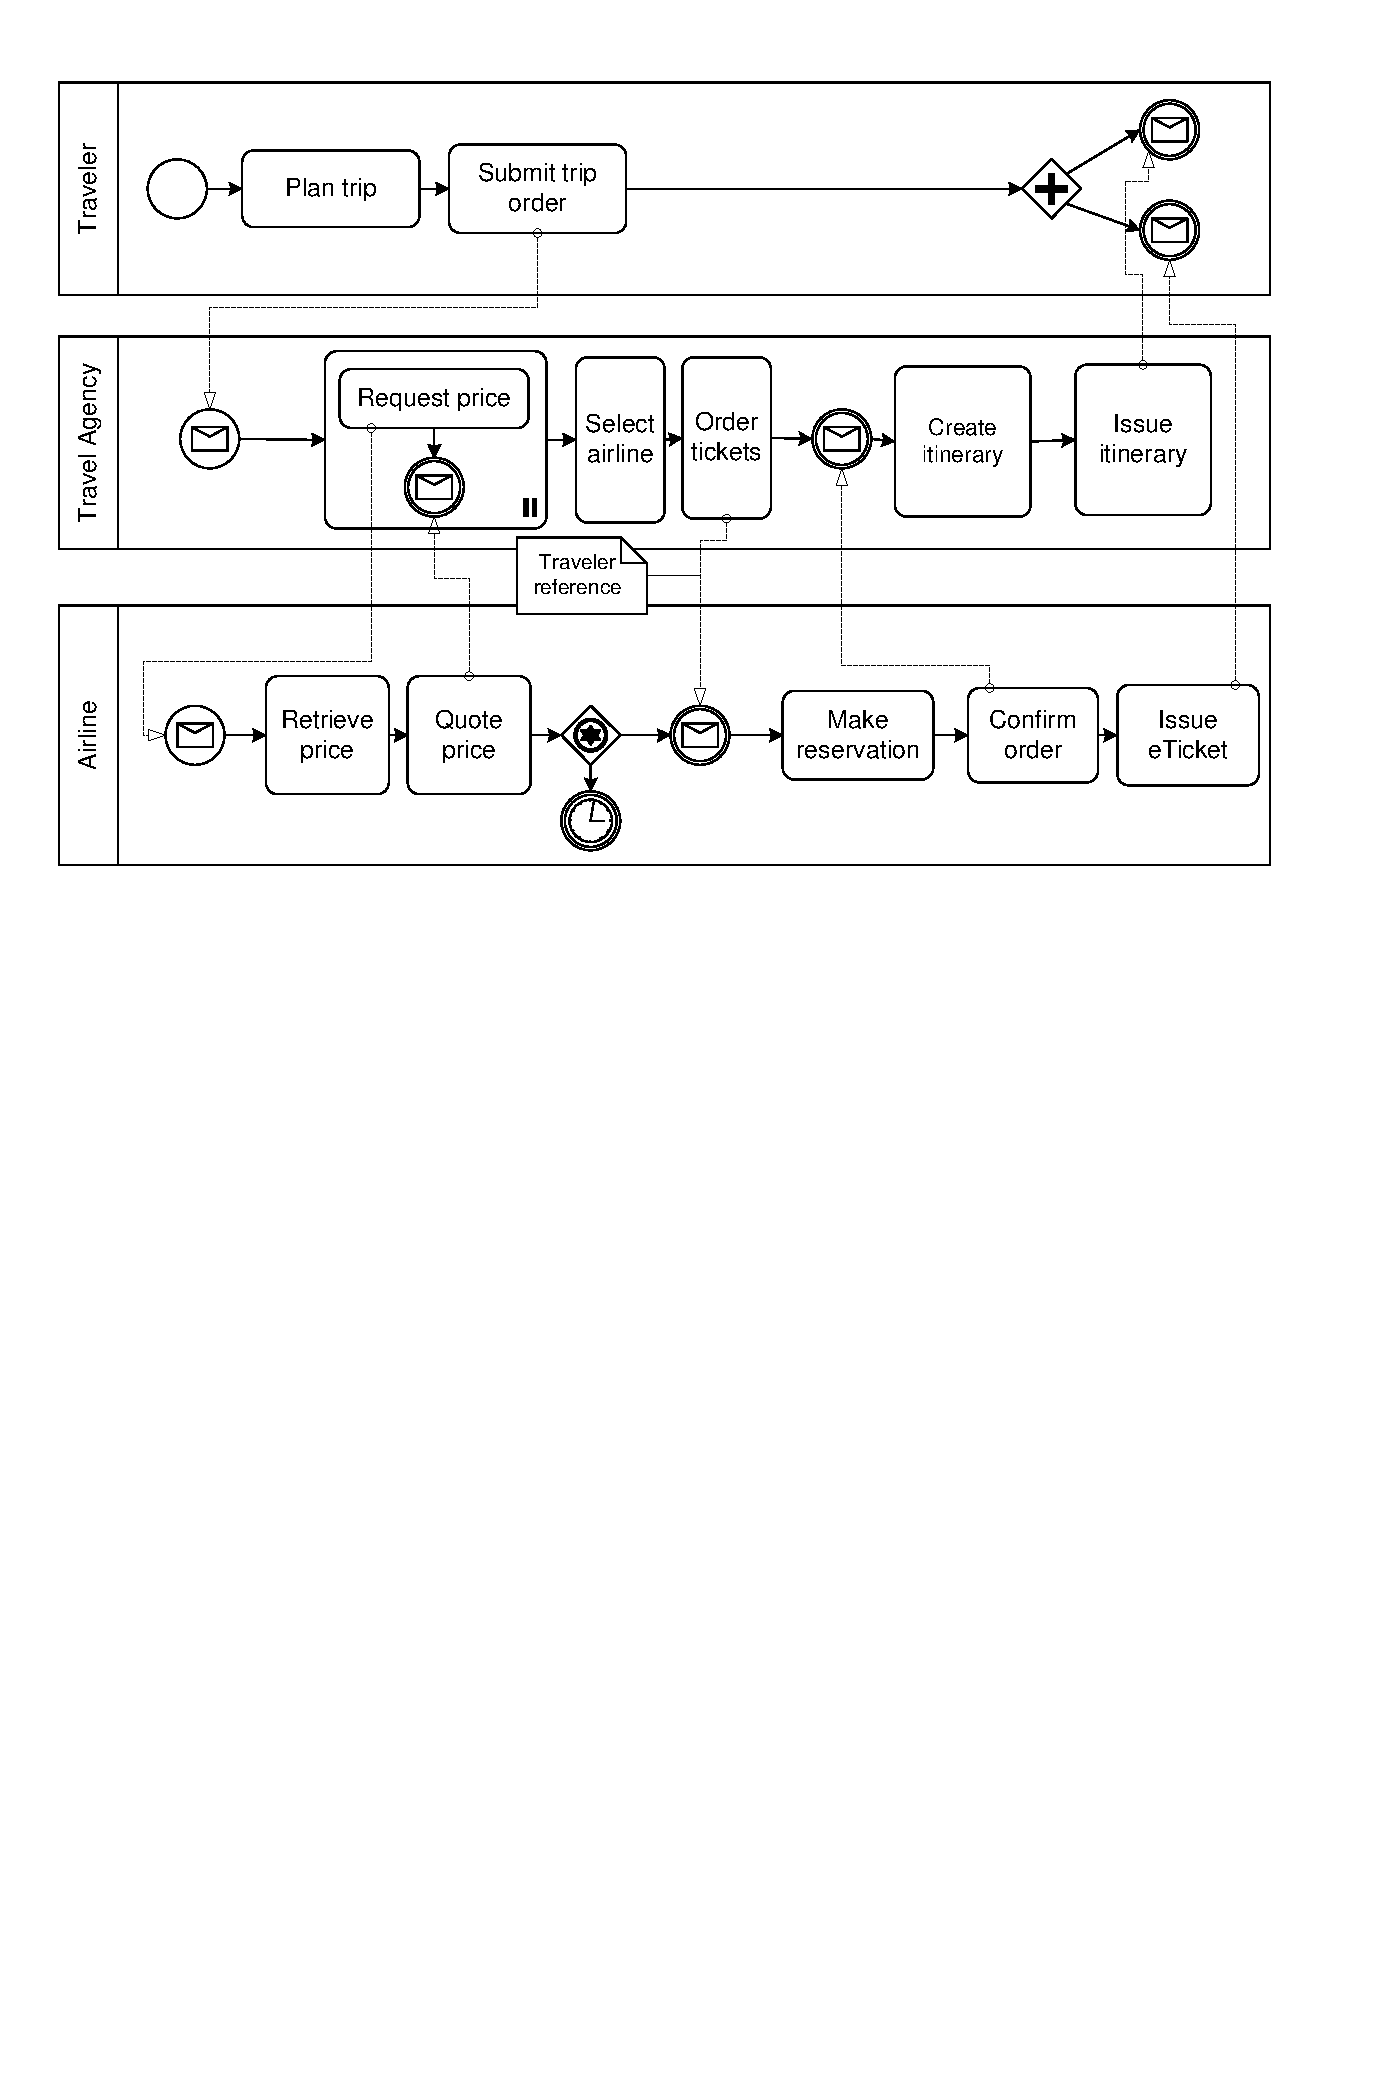
\includegraphics[width=\textwidth]{choreography.pdf}
  \caption{Beispiel-Choreographie I}
  \label{fig:AnhangsChor}
\end{figure}

\begin{landscape}
  \begin{figure}
    \centering
    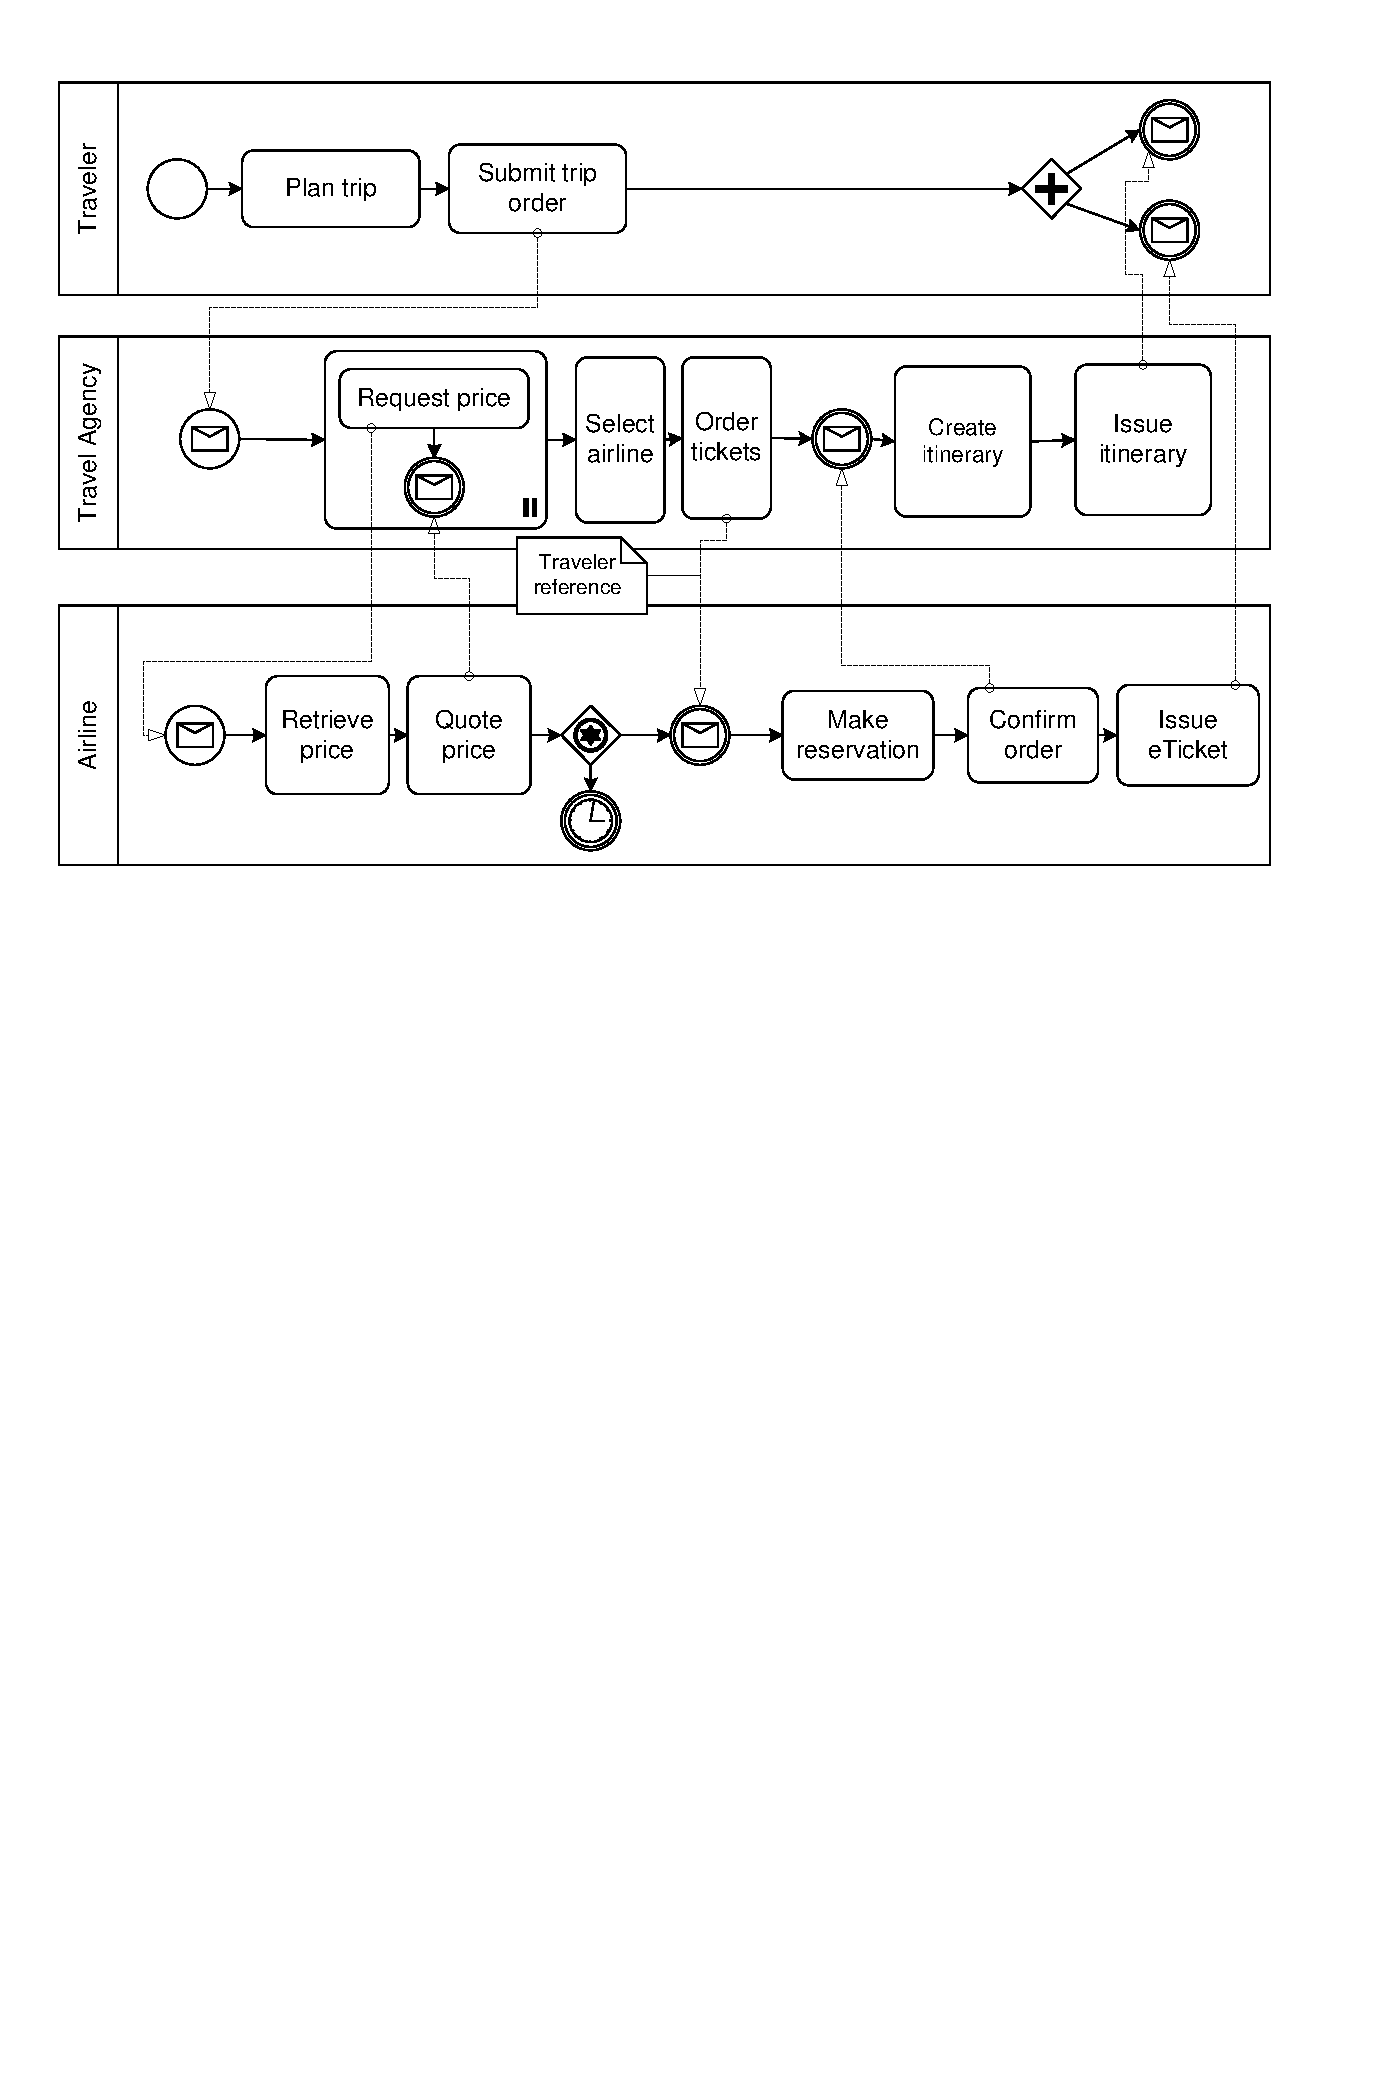
\includegraphics[width=\textwidth]{choreography.pdf}
    \caption{Beispiel-Choreographie II}
    \label{fig:AnhangsChor2}
  \end{figure}
\end{landscape}


\iffalse

\clearpage

FIXME - This does not work with MiKTeX as of 2016-12-30

TODO- demonstrate rotating package

%hint by http://tex.stackexchange.com/a/3265/9075
%other option is to use changepage according to http://tex.stackexchange.com/a/2639/9075. This, however, has issues with landscape
\thispagestyle{empty}

\savegeometry{koma}

%If you only have height problems, this is not needed at all
\addtolength{\textwidth}{2cm}
\addtolength{\evensidemargin}{-1cm}

\begin{landscape}
  %sidewaysfigure
  \begin{figure}
    \centering
    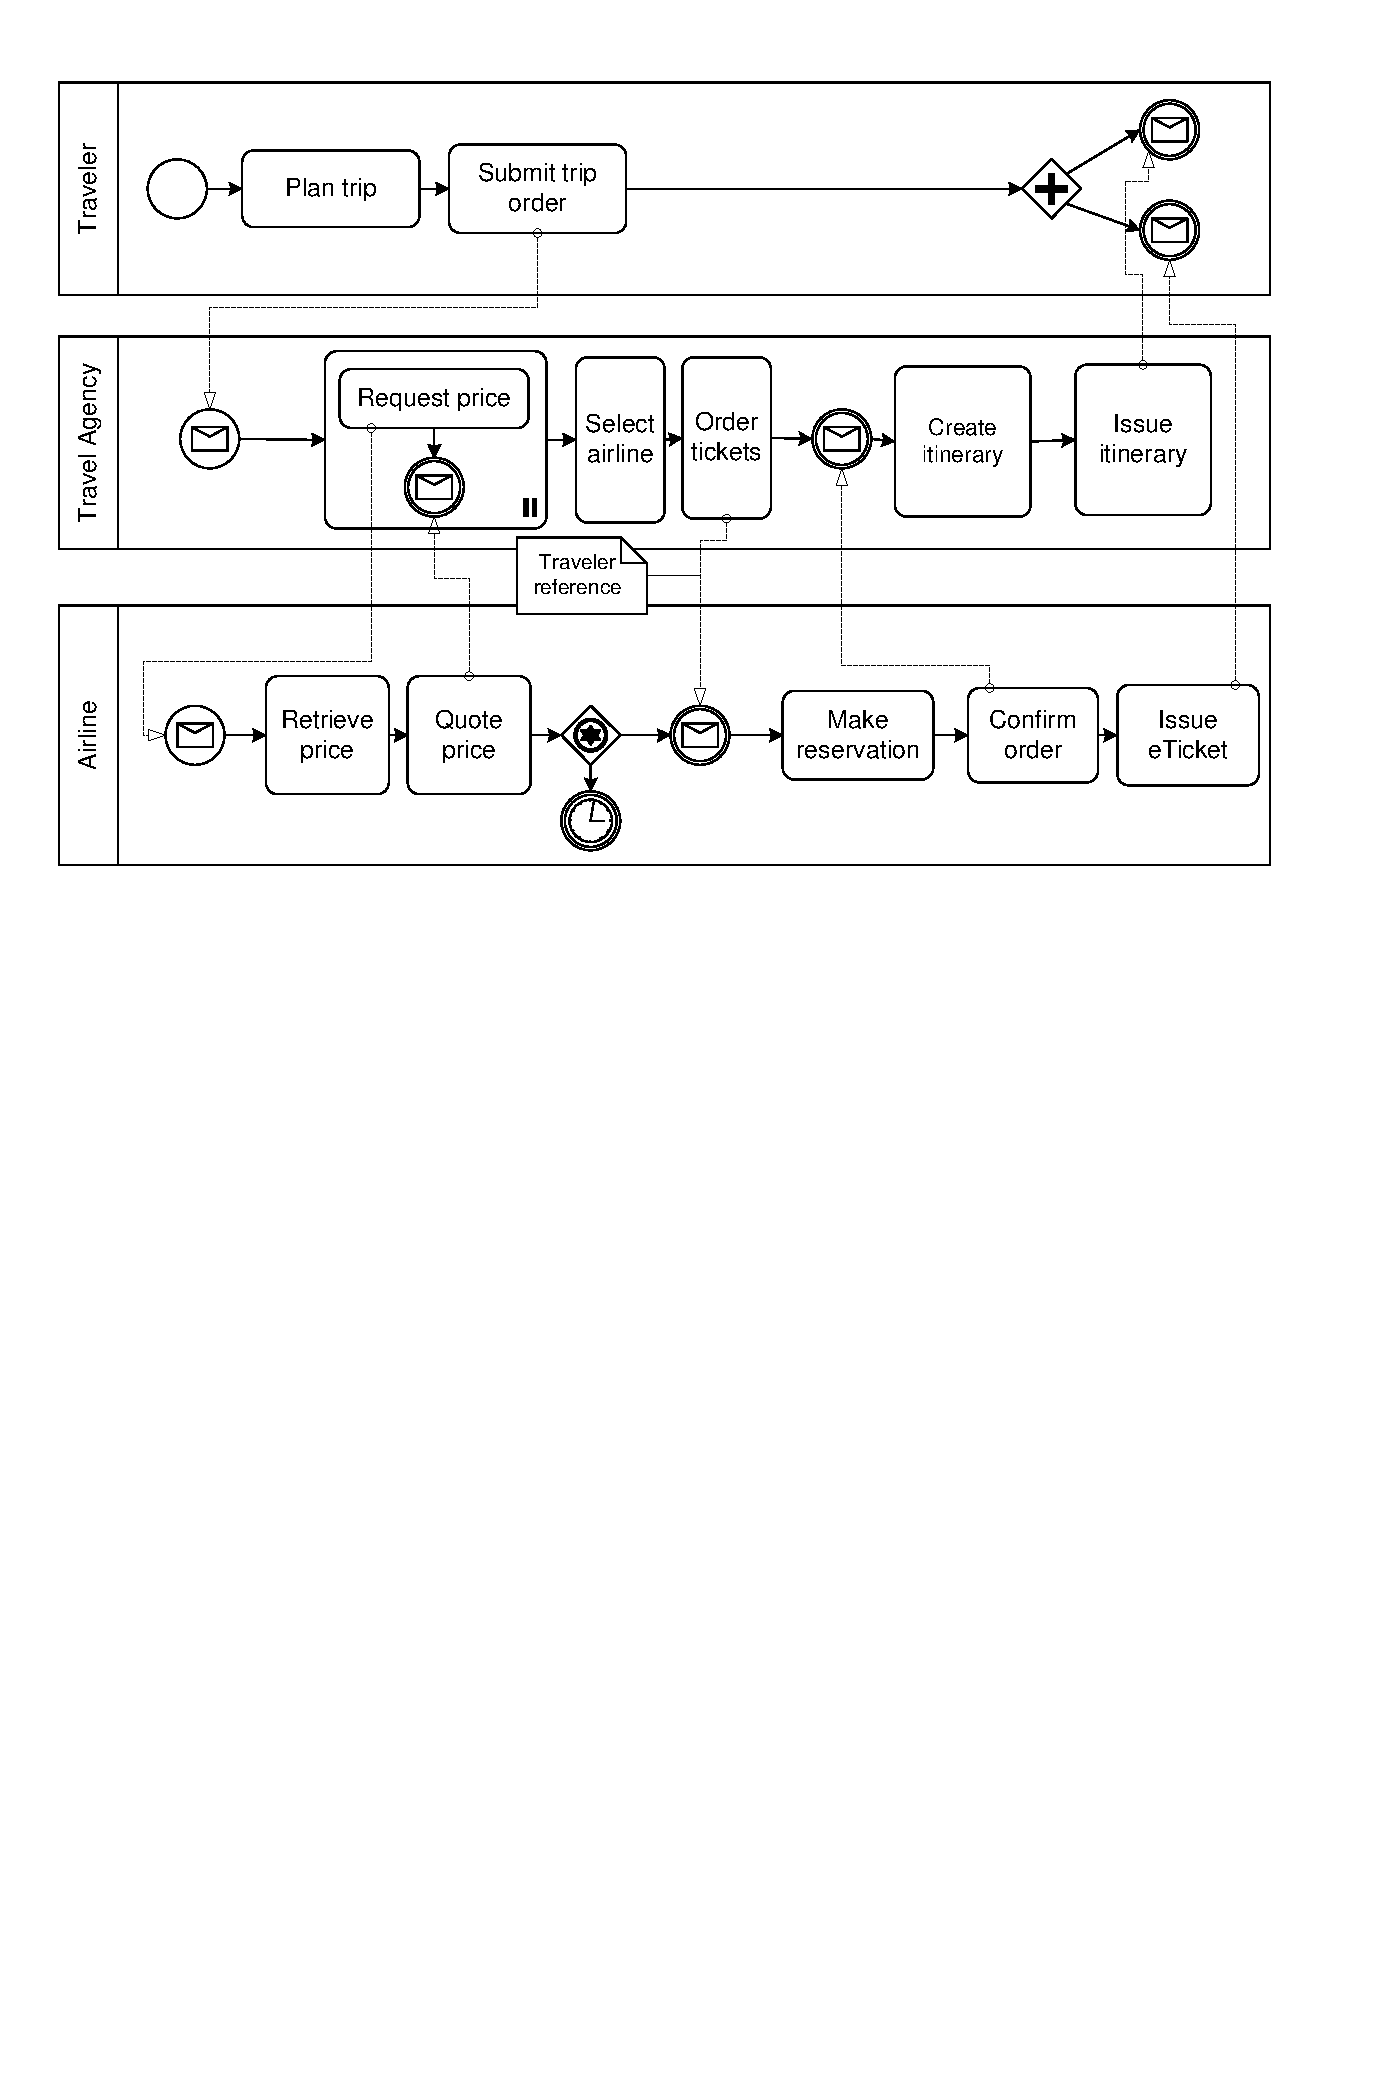
\includegraphics[width=0.9\paperheight]{choreography.pdf}
    \caption{Beispiel-Choreographie, auf einer weißen Seite gezeigt wird und über die definierten Seitenränder herausragt}
  \end{figure}
\end{landscape}

%the original layout is restored.
%%\restoregeometry cannot be used as we use \addtolength
\loadgeometry{koma}

\fi


\IfFileExists{pgfplots.sty}{
\section{Plots with pgfplots}
Pgfplot ist ein Paket um Graphen zu plotten ohne den Umweg über gnuplot oder matplotlib zu gehen.
\begin{figure}[h]
\begin{center}
\begin{tikzpicture}
  \begin{axis}[xlabel=$x$,
               ylabel=$\sin(x)$]
    \addplot {sin(deg(x))};  % Sinus-Funktion zeichnen
  \end{axis}
\end{tikzpicture}
\end{center}
\caption{$\sin(x)$ mit pgfplots.}
\end{figure}
}

\IfFileExists{tikz.sty}{
\section{Figures with tikz}
TikZ ist ein Paket um Zeichnungen mittels Programmierung zu erstellen.
Dieses Paket eignet sich um Gitter zu erstellen oder andere regelmäßige Strukturen zu erstellen.
\begin{figure}[ht]
\begin{center}
\begin{tikzpicture}
  \draw(0,0) rectangle (4,4);
  \foreach \x in {0.5,1,1.5,2,2.5,3,3.5}
    \foreach \y in {0.5,1,1.5,2,2.5,3,3.5}
      \draw(\x,\y) circle (1pt);
\end{tikzpicture}
\end{center}
\caption{Eine tikz-Graphik.}\label{fig:tikz_example}
\end{figure}
}{}

\section{Schlusswort}
Verbesserungsvorschläge für diese Vorlage sind immer willkommen.
Bitte bei GitHub ein Ticket eintragen (\url{https://github.com/latextemplates/uni-stuttgart-computer-science-template/issues}).
%%%%% HERE %%%%%%%%%%%

\clearpage

%\printindex

%\chapter*{Acknowledgements}
%%\thispagestyle{empty}
%
%The author gratefully acknowledges Dr.-Ing. Franz Kurz ...
%
%\clearpage


\printbibliography

\ifdeutsch
Alle URLs wurden zuletzt am 17.\,03.\,2008 geprüft.
\else
All links were last followed on January 31, 2018.
\fi

\pagestyle{empty}
\renewcommand*{\chapterpagestyle}{empty}
\Versicherung
\end{document}
